\documentclass[12pt, a4paper, twoside]{report} 
\usepackage{blindtext}
\usepackage{float}
\usepackage{setspace}
\linespread{1.5}
\usepackage{graphicx}
\usepackage[a4paper,top=3.5cm,bottom=3.5cm,left=2.5cm,right=2.5cm,marginparwidth=1.75cm]{geometry}
\setlength{\headheight}{14.5pt}
\usepackage[colorlinks=true, linkcolor=blue, citecolor=red]{hyperref}
\graphicspath{{./Chapter2/}}
\usepackage{acronym}
\usepackage{amsmath}
\usepackage{amssymb}
\usepackage{fancyhdr}
\usepackage{tikz}
\usepackage{colortbl} % Required for colored table rules
\usepackage{xcolor}    % Provides color definitions
\usepackage{mathtools}
\usepackage{subcaption}
\usepackage[compat=1.1.0]{tikz-feynman}
\definecolor{lightgray}{rgb}{0.8,0.8,0.8} 
\usepackage{adjustbox}
\usepackage[numbers,sort&compress]{natbib}
\usepackage{enumitem}
\setlist[itemize]{topsep=5pt, partopsep=0pt, parsep=0pt, itemsep=0.5\baselineskip}
\usepackage[perpage]{footmisc}

\makeatletter
\g@addto@macro\normalsize{%
  \setlength{\abovedisplayskip}{1pt}%
  \setlength{\belowdisplayskip}{1pt}%
  \setlength{\abovedisplayshortskip}{1pt}%
  \setlength{\belowdisplayshortskip}{1pt}%
}
\makeatother

\usepackage{minitoc}

\usepackage{titlesec}
\titlespacing*{\subsection}{0pt}{1.5ex}{1ex}
\titlespacing*{\subsubsection}{0pt}{1.5ex}{1ex}

\usepackage{indentfirst}
\setlength{\parindent}{15pt}   % Indentation at beginning of paragraphs
\setlength{\parskip}{0.5em}    % Whitespace between paragraphs

\usepackage[Lenny]{fncychap}   % or whatever style you like

\makeatletter
\renewcommand{\DOCH}{%
    \@ifundefined{@chapapp}{\let\@chapapp\chaptername}{}%

    \settowidth{\px}{\CNV\FmN{\@chapapp}}%
    \addtolength{\px}{2pt}%
    \settoheight{\py}{\CNV\FmN{\@chapapp}}%
    \addtolength{\py}{1pt}%
    
    \settowidth{\mylen}{\CNV\FmN{\@chapapp}\space\CNoV\thechapter}%
    \addtolength{\mylen}{1pt}%
    \settowidth{\pxx}{\CNoV\thechapter}%
    \addtolength{\pxx}{-1pt}%
    
    \settoheight{\pyy}{\CNoV\thechapter}%
    \addtolength{\pyy}{-2pt}%
    \setlength{\myhi}{\pyy}%
    \addtolength{\myhi}{-1\py}%
    \par
    \parbox[b]{\textwidth}{%
        \rule[\py]{\RW}{\myhi}%
        \hskip -\RW%
        \rule[\pyy]{\px}{\RW}%
        \hskip -\px%
        \raggedright%
        \CNV\FmN{\@chapapp}\space\CNoV{\color{teal}\thechapter}%
        \hskip1pt%
        \mghrulefill{\RW}%
        \rule{\RW}{\pyy}\par\nobreak%
        \vskip -\baselineskip%
        \vskip -\pyy%
        \hskip \mylen%
        \mghrulefill{\RW}\par\nobreak%
        \vskip \pyy%
    }%
    \vskip 20\p@%
}
\makeatother

% thickness of the box‐rule (optional; adjust to your taste)
\ChNameUpperCase

\ChNameVar{\fontsize{14}{16}\selectfont}
\ChNumVar{\fontsize{60}{62}\selectfont}
\ChTitleVar{\Huge\bfseries}
\ChRuleWidth{1.15pt}

%-------------
% CMS Packages
\usepackage{style/ptdr-definitions}
\usepackage{style/hepparticles}
\usepackage{style/heppennames2}
\usepackage{mathrsfs}
%-------------

\pagestyle{plain}  % Default plain page style
\fancypagestyle{chapterpages}{
    \fancyhf{} % Clear existing header/footer
    \fancyhead[L]{\thepage}  % Left header: Page number
    \fancyhead[R]{\nouppercase{Chapter \thechapter: \leftmark}}
    \renewcommand{\headrulewidth}{0.4pt} % Header rule
}
\renewcommand{\chaptermark}[1]{\markboth{#1}{}}

\newcommand{\hardmaths} {\frac{\sin{(x\pi)}} {2\alpha}}

\newcommand{\diff}[2]  {\frac{\textrm{d}{#1}} {\textrm{d}{#2}}}

% ===== Consistent spacing around math environments =====
\newenvironment{equation_pad}
  {\vspace{-0.5pt}\begin{equation}}
  {\end{equation}\vspace{-0.5pt}}

\newenvironment{align_pad}
  {\vspace{-0.5pt}\begin{align}}
  {\end{align}\vspace{-0.5pt}}

\newenvironment{gather_pad}
  {\vspace{-0.5pt}\begin{gather}}
  {\end{gather}\vspace{-0.5pt}}

\newenvironment{multline_pad}
  {\vspace{-0.5pt}\begin{multline}}
  {\end{multline}\vspace{-0.5pt}}


\begin{document}
\dominitoc

\includegraphics[width=7cm]{IMPERIAL_Wordmark_CMYK_Blue_safe_area_2024.jpg}
\vspace{5cm}
\begin{center}


{\huge Exploring extended Higgs sectors and the CP Nature of the Higgs Yukawa coupling using tau leptons at the CMS Experiment}
\rule{15cm}{1pt}
\vspace{2cm}

Klitos Savva\\
2025
\vspace{2cm}

Department of Physics

Imperial College London
\vspace{2cm}

Submitted in part fulfilment of the requirements for the degree of\\
Doctor of Typessetting of Imperial College London\\
and the Diploma of Imperial College London
\vfill
\clearpage
\end{center}

\chapter*{Abstract}
\blindtext

\chapter*{Statement of Originality}
\blindtext

\chapter*{Copyright Statement}
\blindtext

\tableofcontents
\listoffigures
\listoftables

\clearpage
\section*{List of Acronyms}
\begin{acronym}
\acro{SM}{Standard Model}
\acro{BSM}{Beyond-the-Standard Model}
\acro{QFT}{Quantum Field Theory}
\acro{QED}{Quantum Electrodynamics}
\acro{QCD}{Quantum Chromodynamics}
\acro{BEH}{Brout-Englert-Higgs}
\acro{SSB}{Spontaneous Symmetry Breaking}
\acro{VEV}{Vacuum Expectation Value}
\acro{dof}{Degrees of Freedom}
\acro{LHC}{Large Hadron Collider}
\acro{EFT}{Effective Field Theory}
\acro{SUSY}{Supersymmetry}
\acro{MSSM}{Minimal Supersymmetric Standard Model}
\acro{2HDM}{Two-Higgs Doublet Model}
\acro{FCNC}{Flavour-Changing-Neutral-Currents}
\acro{CMS}{Compact Muon Solenoid}
\acro{MET}{Missing Transverse Energy}
\acro{CERN}{European Organization for Nuclear Research}
\acro{LEP}{Large Electron Positron}
\acro{LINAC4}{Linear Accelerator 4}
\acro{PSB}{Proton Synchrotron Booster}
\acro{PS}{Proton Synchrotron}
\acro{SPS}{Super Proton Synchrotron}
\acro{PU}{Pileup}
\acro{ECAL}{Electromagnetic Calorimeter}
\acro{HCAL}{Hadronic Calorimeter}
\acro{BPIX}{Barrel Pixel}
\acro{FPIX}{Forward Pixel}
\acro{SST}{Silicon Strip Tracker}
\acro{TIB}{Tracker Inner Barrel}
\acro{TID}{Tracker Inner Disks}
\acro{TOB}{Tracker Outer Barrel}
\acro{TEC}{Tracker EndCaps}
\acro{APDs}{Avalanche Photodiodes}
\acro{VPTs}{Vacuum Phototriodes}
\acro{HB}{Hadron Barrel}
\acro{HE}{Hadron Endcap}
\acro{HO}{Hadron Outer}
\acro{HF}{Hadron Forward}
\acro{DTs}{Drift Tubes}
\acro{CSCs}{Cathode Strip Chambers}
\acro{RPC}{Resistive Plate Chamber}
\acro{L1}{Level-1}
\acro{HLT}{High Level Trigger}
\end{acronym}

%\chapter{The Standard Model of particle physics}
\chaptermark{The Standard Model of particle physics}  
\thispagestyle{plain}  % First page has default style
\pagestyle{chapterpages}
\label{Section:Chapter1}

\minitoc

The \ac{SM} of particle physics~\cite{Glashow_1, Weinberg_1, Salam_1, MarkThompson}\footnote{References~\cite{Glashow_1, Weinberg_1, Salam_1} correspond to the foundational works on electroweak unification, while Reference~\cite{MarkThompson} provides an accessible and comprehensive textbook overview of the entire \ac{SM}.} is our current best theoretical framework underpinning our understanding of the subatomic world. It provides a description of fundamental elementary particles and their interactions via the \textit{electromagnetic force}, \textit{weak nuclear force} and \textit{strong nuclear force}. The fourth fundamental force of nature, \textit{gravity}, is absent from the \ac{SM}, highlighting one of its key limitations. However, in high-energy physics experiments, where the interactions of subatomic particles are being studied, the omission of gravity is considered a safe simplification. Extremely powerful predictions have emerged from this theoretical framework, with its greatest accomplishments being the prediction~\cite{Englert_Brout,PeterHiggs_1,PeterHiggs_2, PeterHiggs_3, Guralnik_Hagen_Kibble, Kibble} and subsequent discovery of the \textit{Higgs boson} in 2012~\cite{Higgs_ATLAS,Higgs_CMS}. Despite its success, the \ac{SM} has its limitations. Along with the absence of gravity, it leaves several fundamental questions unanswered, such as the nature of \textit{neutrino oscillations}~\cite{Neutrino_Oscillations, Neutrino_Oscillations_2}, the existence of \textit{dark matter}~\cite{DarkMatter_1,DarkMatter_2,DarkMatter_3}\footnote{Reference~\cite{DarkMatter_1} is a modern English translation of Zwicky's seminal 1933 paper, which first proposed the concept of dark matter}, the \textit{hierarchy problem}~\cite{HierarchyProblem}, and the \textit{matter-antimatter asymmetry} in the universe~\cite{MatterAntimatter}. These have been driving the field to look for explanations beyond the \ac{SM}. In the pursuit of \ac{BSM} physics, a deep understanding of the \ac{SM} theory is crucial. The goal of this chapter is to establish the base foundation for this work, the \ac{SM}, by exploring the fundamental blocks of the theory.

\section{Particle content and fundamental interactions}
\label{Section:Particle content and fundamental interactions}
Built on the theoretical framework of \ac{QFT}, the \ac{SM} is a renormalisable theory. In this theory, the physical particles observed in nature, referred to as \textit{fermions}, emerge as quantised excitations of underlying relativistic fields. Force carriers mediate their interactions, \textit{vector bosons}, and together, these two groups of particles constitute the particle content of the \ac{SM}, as shown in Fig.~\ref{Figure:Introduction_1}.

\begin{figure}[ht]
\centering
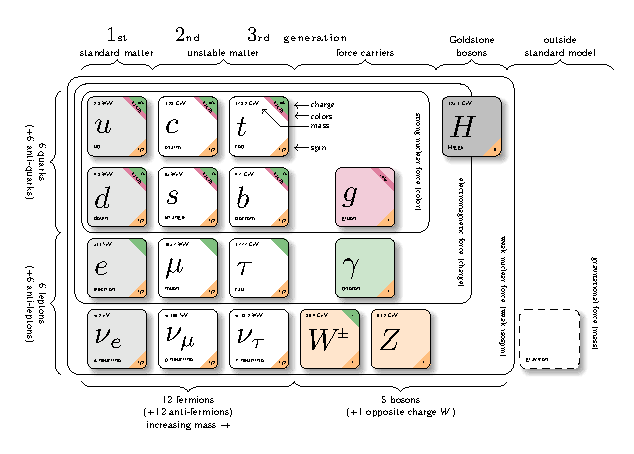
\includegraphics[width= 0.9\textwidth]{Figures/Introduction/Particles.pdf}
\caption[Diagram of the particle content of the Standard Model]{Diagram of the particle content of the \ac{SM}. For each fundamental particle, the charges, colour and spin quantum numbers are available. The measured masses for all fermions and gauge bosons are taken from Ref.~\cite{ParticleMasses} with the exception of the Higgs mass, which is taken from Ref.~\cite{Higgs_Mass}.}
\label{Figure:Introduction_1}
\end{figure}

Within the \ac{SM}, fermions serve as the fundamental constituents of all observable matter. These elementary, non-composite, spin-1/2 particles are organised into three distinct generations, with each fermion paired with an antiparticle. The antiparticles exhibit quantum numbers precisely opposite in sign, with the exception of mass and spin, which remain identical. As shown in Fig.~\ref{Figure:Introduction_1}, fermions are further divided into \textit{quarks} and \textit{leptons}. 

The leptonic sector consists of three charged leptons (\textit{electron, muon, tau}) and three electrically neutral neutrinos (\textit{electron neutrino, muon neutrino, tau neutrino}). The quark sector, on the other hand, comprises of six quark flavours; \textit{up}, \textit{down}, \textit{charm}, \textit{strange}, \textit{top} and \textit{bottom}. Within the first generation, the electron and electron neutrino comprise the leptons, while the up and down quarks form the quark sector. Although fundamental quantum numbers remain identical across generations\footnote{While fundamental quantum numbers like electric charge remain constant, others, such as flavour, vary across generations, as do properties like mass.}, the mass spectrum exhibits a strong hierarchy, with the third generation being significantly heavier than the first.

A key distinction between leptons and quarks lies in their participation in strong interactions. Unlike leptons, quarks possess an additional quantum number known as a colour charge, enabling their interactions via the strong force, which is mediated by massless gluons ($\Pg$). In addition to the strong interaction, charged leptons and quarks interact electromagnetically due to their electric charge, with massless photons ($\PGg$) acting as the mediators of the force. Conversely, neutrinos, being electrically neutral, do not participate in electromagnetic interactions. All fermions, including neutrinos, interact via the weak interaction, which occurs via the exchange of massive vector bosons, $\PW^\pm$ bosons and $\PZ$ bosons. These fundamental interactions are explored in more detail in the following section.

\section{Foundation of the fundamental interactions}
\label{Section:Chapter1_FundamentalInteractions}

Symmetries describing the fundamental interactions are the core of the \ac{SM}. N\"{o}ether's theorem~\cite{Noether_1,Noether_2}\footnote{Reference~\cite{Noether_1} is an english translation of N\"{o}ether's original paper.} shows that a conservation law is implied by the invariance of a Lagrangian under a continuous transformation (symmetry). A striking example of the deep connection between fundamental interactions and symmetry principles is the conservation of angular momentum, defined by a Lagrangian, which is invariant under rotational transformations. 

The \ac{SM} is a \textit{gauge theory} built on the principle of \textit{local gauge invariance} \ie the Lagrangian is invariant under local phase transformations. Such transformations shift the phase of the field ($\psi(x)$) as a function of the spacetime coordinates

\begin{equation_pad}
    \psi(x) \rightarrow e^{iq\theta(x)} \psi(x)
\label{Equation:Introduction_LocalPhaseTransformation}
\end{equation_pad}

where $q$ is the charge associated with the gauge symmetry and 
$\theta(x)$ is a \\ spacetime-dependent function representing the local phase transformation. The introduction of the gauge boson fields mediating fermion interactions is a direct consequence of imposing this invariance. Alone, a local phase transformation would break the invariance of the \ac{SM} Lagrangian, which is restored by the introduction of the gauge boson fields.

\subsection{Quantum Electrodynamics}
The \ac{QFT} of electromagnetism, known as \textbf{\ac{QED}}~\cite{QED}, describes the interactions between electrically charged fermions through the exchange of photons. Remarkably, the entire framework of \ac{QED} emerges beautifully from a single guiding principle: \textit{the requirement that the \ac{QED} Lagrangian remains invariant under local $\mathcal{U}$(1) gauge transformations}. The foundation of \ac{QED} begins with the Dirac equation \cite{MarkThompson} which describes the equations of motion for spin-$\frac{1}{2}$ fermion fields,

\begin{equation_pad}
    \mathcal{L}_{\text{Dirac}} = \overline{\psi}(i\gamma^\mu \partial_\mu - m_{\psi}) \psi
\label{Equation:Introduction_DiracEquation}
\end{equation_pad}

where $\psi$ and its adjoint $\overline{\psi}$ are the fermion fields expressed as four-component Dirac spinors while the quantity $\gamma^\mu$ represents the Dirac gamma matrices. Finally, $m_{\psi}$ represents the mass of the fermion.

As briefly discussed in Section~\ref{Section:Chapter1_FundamentalInteractions}, under a local $\mathcal{U}$(1) gauge transformation, the fermion field transforms in a way (Eq.~\ref{Equation:Introduction_LocalPhaseTransformation}) that breaks the local gauge invariance of the Lagrangian. Under this transformation, the Dirac equation (Eq.~\ref{Equation:Introduction_DiracEquation}) becomes

\begin{equation_pad}
    \mathcal{U}(1) \rightarrow \mathcal{L}_{\text{Dirac}}^{\prime} = \mathcal{L}_{\text{Dirac}} - q\overline{\psi}\gamma^\mu(\partial_\mu\theta(x))\psi
\label{Equation:Introduction_Dirac(U1)}
\end{equation_pad}

To restore local gauge invariance, the derivative $\partial_\mu$ is replaced with the covariant derivative $D_\mu$,

\begin{equation_pad}
    \partial_\mu \rightarrow D_\mu = \partial_\mu + iqA_\mu
\end{equation_pad}

where $A_\mu$ is a new field. The problematic term in Eq.\ref{Equation:Introduction_Dirac(U1)} can be cancelled out provided that the new field transforms as

\begin{equation_pad}
    \mathcal{U}(1) \rightarrow A_\mu^{\prime} = A_\mu - \partial_\mu \theta(x) 
\end{equation_pad}

Therefore, imposing a $\mathcal{U}$(1) local gauge invariance on the Lagrangian has forced the existence of a photon field, $A_\mu$, with well-defined gauge transformation properties. The local gauge-invariant Lagrangian for a spin-1/2 fermion field becomes

\begin{equation_pad}
    \mathcal{L}_{\text{Dirac}} = \overline{\psi}(i\gamma^\mu \partial_\mu - m_{\psi}) \psi - q\overline{\psi}\gamma^\mu A_\mu\psi
\label{Equation:Dirac_GaugeInvariant}
\end{equation_pad}

The additional term in the Lagrangian (Eq.\ref{Equation:Dirac_GaugeInvariant}) encapsulates the electromagnetic interaction between charged fermions and photons. The strength of this coupling is given by $q = |e|Q$, where e denotes the fundamental unit of electric charge, and Q represents the dimensionless charge of the fermion field $\psi$ relative to e. By N\"{o}ether's theorem, electric charge corresponds to the conserved quantity associated with a local $\mathcal{U}$(1) gauge symmetry, once again reinforcing the deep connection between symmetry and conservation laws in \ac{QFT}. The final component necessary to complete the \ac{QED} Lagrangian is the gauge-invariant kinetic term for the massless spin-1 field, described by the field strength tensor $F_{\mu\nu}$. Incorporating this, the total \ac{QED} Lagrangian takes the form,

\begin{equation_pad}
    \mathcal{L}_{\text{QED}} = \overline{\psi}(i\gamma^\mu \partial_\mu - m_{\psi}) \psi - q\overline{\psi}\gamma^\mu A_\mu\psi - \frac{1}{4}F_{\mu\nu}F^{\mu\nu}
\label{Equation:QED_GaugeInvariant}
\end{equation_pad}

\begin{equation_pad}
F_{\mu\nu} = \partial_\mu A_\nu - \partial_\nu A_\mu
\end{equation_pad}

\subsection{Quantum Chromodynamics}

The \ac{QFT} describing the strong interaction is known as \textbf{\ac{QCD}}. \ac{QCD} governs the dynamics of quarks and gluons, and \textit{it is formulated as a non-Abelian gauge theory under the local $\mathcal{SU}(3)_C$ symmetry group}. While \ac{QED} applies universally to all charged particles, the gauge symmetry of \ac{QCD} only applies to fields that carry colour charge, as denoted by the subscript $C$.

Unlike the Abelian $\mathcal{U}$(1) symmetry of \ac{QED}, which involves a single generator, the $\mathcal{SU}(3)$ symmetry group is represented by eight generators, $T^a$. To ensure local $\mathcal{SU}(3)_C$ gauge invariance, the derivative $\partial_\mu$ is replaced with the covariant derivative expressed in terms of the generators as

\begin{equation_pad}
    \partial_\mu \rightarrow D_\mu = \partial_\mu + ig_sG^{a}_{\mu}T^{a}
\end{equation_pad}

where $G^{a}_{\mu}$ represent the eight new fields, which correspond to the eight massless gluons mediating the strong interaction. The term $g_s$ encodes the coupling strength of the interaction. The full \ac{QCD} Lagrangian can then be expressed as

\begin{equation_pad} 
\mathcal{L}_{\text{QCD}} = \sum_{f}\overline{\psi_f}(i\gamma^\mu D_\mu - m_f)\psi_f - \frac{1}{4} G^{\mu\nu}_{a}G^{a}_{\mu\nu}
\end{equation_pad}

where $\psi_f$ represents the quark field (spinor) for the $f^{th}$ flavour. Once again, according to N\"{o}ether's theorem, colour charge corresponds to the conserved quantity associated with local $\mathcal{SU}(3)_C$ gauge symmetry.

Unlike \ac{QED}, the kinetic (gauge term) in the Lagrangian includes additional terms representing the self-interactions of the gauge bosons. This is a direct consequence of the \ac{QCD} generators not commuting,

\begin{equation_pad}
    [T^a,T^b] = if^{abc}T^c
\end{equation_pad}

which allows gluons themselves to carry colour charge. The quantity $f^{abc}$ refers to the structure constants of the symmetry group. This gluon self-interaction property modifies the strength of the interaction ($\alpha_{S}$), causing it to decrease as a function of the interaction energy scale. Hence, $\alpha_{S}$ is referred to as a running coupling constant.

An important consequence of this is \textit{asymptotic freedom}~\cite{AsymptoticFreedom_1,AsymptoticFreedom_2}, where at very high energies (short distances), such as the deep scattering energies at the \ac{LHC}, $\alpha_{S}$ decreases approaching zero. In this scenario, quarks and gluons behave as quasi-free particles within the protons and neutrons, allowing perturbative \ac{QCD} to describe their interactions accurately. However, at low energies, the strong coupling grows large, making \ac{QCD} non-perturbative. In this regime, quarks and gluons are not found as free particles but instead form bound, colour-neutral states known as hadrons. This phenomenon, known as \textit{colour confinement}~\cite{MarkThompson}\footnote{The phenomenon of colour confinement was first motivated theoretically in the 1970s through ideas such as flux tube formation and asymptotic freedom. A clear summary is provided in Reference~\cite{MarkThompson}.}, ensures that isolated colour-charged particles do not exist in nature; only hadrons are observed.

As a consequence of colour confinement, in high-energy collisions, high-energy quarks and gluons are observed as jets~\cite{Hadronisation_Jets} of colourless particles formed through a process known as hadronisation. In the context of proton-proton (pp) collisions, highly energetic partons fly away from the interaction point. As the partons separate, the colour field between them can be thought of as if it is being squeezed in a tube, with the energy in the field becoming increasingly larger with distance. Once that energy becomes sufficient, a new quark-antiquark pair is produced, separating the colour field into smaller segments. Eventually, the formation of colourless hadrons occurs when the quark-antiquark pairs have sufficiently low energy. This resulting cascade of collimated hadrons forms what is observed as a jet. A qualitative schematic of the hadronisation process is shown in Fig.~\ref{Figure:Introduction_ColourConfinement}.

\begin{figure}[h]
    \centering
    \begin{tikzpicture}[>=stealth,thick]

%----------------- (i) -----------------%
\node at (-2,0) {\large (i)};
% Quark & antiquark with arrows
\node[circle, fill=black, scale=0.7, label=above:$q$] (q_i) at (4.5,0) {};
\node[circle, fill=black, scale=0.7, label=above:$\bar{q}$] (qb_i) at (5.5,0) {};
\draw[->] (q_i) -- ++(-1.5, 0);
\draw[->] (qb_i) -- ++(+1.5, 0);

%----------------- (ii) -----------------%
\node at (-2,-1.5) {\large (ii)};
% Another q/qbar pair with a flux tube (string)
\node[circle, fill=black, scale=0.7, label=above:$q$] (q_ii) at (3.5,-1.5) {};
\node[circle, fill=black, scale=0.7, label=above:$\bar{q}$] (qb_ii) at (6.5,-1.5) {};
% Draw the string (solid line) plus double arrow to suggest tension
\draw[thick] (q_ii) to[out=20, in=160] (qb_ii);
\draw[thick] (q_ii) to[out=-20, in=-160] (qb_ii);
\draw (q_ii) -- (qb_ii);
\draw[->] (q_ii) -- ++(-1.5, 0);
\draw[->] (qb_ii) -- ++(+1.5, 0);

%----------------- (iii) -----------------%
\node at (-2,-3.0) {\large (iii)};
% Multiple q/qbar pairs horizontally
\node[circle, fill=black, scale=0.7, label=above:$q$] (q1_iii)  at (2.5, -3.0) {};
\node[circle, fill=black, scale=0.7, label=above:$\bar{q}$] (qb1_iii) at (4.5, -3.0) {};
\node[circle, fill=black, scale=0.7, label=above:$q$] (q2_iii)  at (5.5, -3.0) {};
\node[circle, fill=black, scale=0.7, label=above:$\bar{q}$] (qb2_iii)at (7.5, -3.0) {};

\draw[thick] (q1_iii) to[out=20, in=160] (qb1_iii);
\draw[thick] (q1_iii) to[out=-20, in=-160] (qb1_iii);
\draw[thick] (q2_iii) to[out=20, in=160] (qb2_iii);
\draw[thick] (q2_iii) to[out=-20, in=-160] (qb2_iii);

\draw (q1_iii) -- (qb1_iii);
\draw (q2_iii) -- (qb2_iii);

\draw[->] (q1_iii) -- ++(-1.5, 0);
\draw[->] (qb2_iii) -- ++(+1.5, 0);

%----------------- (iv) -----------------%
\node at (-2,-4.5) {\large (iii)};
% Multiple q/qbar pairs horizontally
\node[circle, fill=black, scale=0.7] (q11_iv)  at (1.5, -4.5) {};
\node[circle, fill=black, scale=0.7] (qb11_iv) at (2.5, -4.5) {};
\node[circle, fill=black, scale=0.7] (q12_iv)  at (3, -4.5) {};
\node[circle, fill=black, scale=0.7] (qb12_iv) at (4, -4.5) {};

\node[circle, fill=black, scale=0.7] (q21_iv)  at (5.5, -4.5) {};
\node[circle, fill=black, scale=0.7] (qb21_iv)at (6.5, -4.5) {};
\node[circle, fill=black, scale=0.7] (q22_iv)  at (7, -4.5) {};
\node[circle, fill=black, scale=0.7] (qb22_iv)at (8, -4.5) {};

\draw[thick] (q11_iv) to[out=20, in=160] (qb11_iv);
\draw[thick] (q11_iv) to[out=-20, in=-160] (qb11_iv);
\draw[thick] (q12_iv) to[out=20, in=160] (qb12_iv);
\draw[thick] (q12_iv) to[out=-20, in=-160] (qb12_iv);

\draw[thick] (q21_iv) to[out=20, in=160] (qb21_iv);
\draw[thick] (q21_iv) to[out=-20, in=-160] (qb21_iv);
\draw[thick] (q22_iv) to[out=20, in=160] (qb22_iv);
\draw[thick] (q22_iv) to[out=-20, in=-160] (qb22_iv);

\draw (q11_iv) -- (qb11_iv);
\draw (q12_iv) -- (qb12_iv);
\draw (q21_iv) -- (qb21_iv);
\draw (q22_iv) -- (qb22_iv);

\draw[->] (q11_iv) -- ++(-1.5, 0);
\draw[->] (qb22_iv) -- ++(+1.5, 0);
%----------------- (v) -----------------%
\node at (-2,-6.5) {\large (v)};
% Final hadrons on the left
\node[draw, circle, scale=1.0] (H1_v) at (1.5,-6) {};
\node[draw, circle, scale=1.0] (H2_v) at (1.7,-7) {};
\node[draw, circle, scale=1.0] (H3_v) at (2.5,-6.2) {};
\node[draw, circle, scale=1.0] (H4_v) at (2,-6.4) {};

% Arrows indicating motion outward
\draw[->] (1.2,-6) -- ++(-0.7, 0.6);
\draw[->] (1.2,-6.2) -- ++(-0.7, 0.4);
\draw[->] (1.2,-6.4) -- ++(-0.7, 0.2);
\draw[->] (1.2,-6.6) -- ++(-0.7, -0.2);
\draw[->] (1.2,-6.8) -- ++(-0.7, -0.4);
\draw[->] (1.2,-7) -- ++(-0.7, -0.6);

% Final hadrons on the right
\node[draw, circle, scale=1.0] (H5_v) at (8,-6) {};
\node[draw, circle, scale=1.0] (H6_v) at (7.8,-7) {};
\node[draw, circle, scale=1.0] (H7_v) at (7,-6.2) {};
\node[draw, circle, scale=1.0] (H8_v) at (7.5,-6.4) {};
\draw[->] (8.3,-6) -- ++(0.7, 0.6);
\draw[->] (8.3,-6.2) -- ++(0.7, 0.4);
\draw[->] (8.3,-6.4) -- ++(0.7, 0.2);
\draw[->] (8.3,-6.6) -- ++(0.7, -0.2);
\draw[->] (8.3,-6.8) -- ++(0.7, -0.4);
\draw[->] (8.3,-7) -- ++(0.7, -0.6);

\end{tikzpicture}
    \caption{Qualitative schematic of the steps involved in the hadronisation process.}
    \label{Figure:Introduction_ColourConfinement}
\end{figure}

\subsection{Electroweak theory}

In the 1960s, Glashow~\cite{Glashow_1}, Salam~\cite{Salam_1} and Weinberg~\cite{Weinberg_1} discovered that \textit{a unified picture of the electromagnetic and weak interactions} could be constructed. They proposed to develop the electroweak theory incorporating the characteristics of both interactions by associating them with the $\mathcal{SU}(2)_{L}$ $\otimes$ $\mathcal{U}(1)_{Y}$ symmetry group,

\begin{equation_pad}
    \mathcal{SU}(2)_L \otimes \mathcal{U}(1)_Y \rightarrow \mathcal{L}^{\prime}_{\text{EW}} = \mathcal{L}_{\text{EW}}
\end{equation_pad}

where $L$ denotes the \textit{left-handed nature} of the weak interaction under $\mathcal{SU}(2)_L$, and $Y$ represents the \textit{weak hypercharge} associated with the $\mathcal{U}(1)_Y$ gauge symmetry. To ensure that the electroweak Lagrangian is invariant under local transformations of this symmetry group, the covariant derivative is written as

\begin{equation_pad}
    D_\mu = \partial_\mu + \underbrace{ig^{\prime}B_\mu Y}_{\mathcal{U}(1)_Y} + \underbrace{\frac{i}{2}gW^i_\mu\sigma^i}_{\mathcal{SU}(2)_L}
\end{equation_pad}

where $Y$ is the single generator of the $\mathcal{U}(1)_Y$ gauge group, associated with the gauge boson field, $B_\mu$. While the three generators of $\mathcal{SU}(2)_L$ are represented by the 2 x 2 Pauli-spin matrices ($\sigma^i$), associated with the three gauge boson fields, $W^i_\mu$. The coupling strengths of the interactions are represented by $g$ and $g^{\prime}$, respectively. The conserved charges corresponding to these gauge symmetries are the weak isospin component, $I_3$, for $\mathcal{SU}(2)_L$ and the weak hypercharge, Y, for $\mathcal{U}(1)_Y$.

By imposing gauge invariance under the electroweak symmetry group, four gauge fields arise: the three weak isospin fields, $W_{\mu}^{(i)}$ (i=1,2,3), and the weak hypercharge field, $B_{\mu}$. These gauge fields can be expressed in terms of the physical bosons as,

\begin{equation_pad}
\begin{array}{c}
A_{\mu} = + B_{\mu} \cos{\theta_{W}} + W_{\mu}^{(3)} \sin{\theta_{W}}, \\
Z_{\mu} = - B_{\mu} \sin{\theta_{W}} + W_{\mu}^{(3)} \cos{\theta_{W}}, \\
W_{\mu}^{\pm} = \frac{1}{\sqrt{2}} (W_{\mu}^{(1)} \mp iW_{\mu}^{(2)}),
\end{array}
\label{Equation:Introduction_PhysicalGaugeFields}
\end{equation_pad}

where $\theta_{W}$, the weak mixing angle, quantifies the mixing between the weak isospin and hypercharge gauge fields. It is related to the weak and electromagnetic coupling constants, $g$ and $g^{\prime}$, by

\begin{equation_pad}
    \theta_W = \text{arctan}(\frac{g^{\prime}}{g})
\end{equation_pad}

As discussed earlier in Section~\ref{Section:Particle content and fundamental interactions}, all fermions interact via the weak interaction. A key feature of the weak interaction is its violation of parity symmetry~\cite{ParityViolation_Wu}. This means that weak interactions exhibit different behaviours under spatial inversions. In contrast to \ac{QED} and \ac{QCD}, which conserve parity and involve pure vector interactions of the form,

\begin{equation_pad}
    j^\mu = \overline{u}\gamma^\mu u
\end{equation_pad}

the weak interaction is required to take a different form to account for its parity-violating nature.

Mathematically, the proper parity transformations can be achieved by requiring the interaction to have a chiral structure. Naturally, this leads to either a V-A or V+A (Vector, Axial Vector) current. Experimentally, it is well established that the weak interaction exhibits a V-A charged current of the form,

\begin{equation_pad}
    j^\mu_{\text{weak}} = \overline{u}\gamma^\mu \frac{1}{2}(1-\gamma^5)u
\label{Equation:Chapter1-WeakChargedCurrent}
\end{equation_pad}

Using chiral operators, $P_{L/R}$, the fermion spinor fields ($u$) can be decomposed into left-handed ($u_{L}$) and right-handed ($u_{R}$) chiral components. 

\begin{equation_pad}
\begin{array}{c}
    P_{L/R} = \frac{1}{2}(1\mp \gamma^5) \quad ,\quad \gamma^5 = \gamma^0\gamma^1\gamma^2\gamma^3 \\
    u = P_Ru +P_Lu = u_R + u_L
\end{array}
\end{equation_pad}

This chiral decomposition is fundamental in the EW theory, only allowing interactions between left-handed fermions (and equivalently, right-handed anti-fermions) and the weak isospin gauge bosons $W_{\mu}^{(i)}$. This can be explicitly seen by substituting the decomposed spinor field ($u$) into the weak charged current (Eq.~\ref{Equation:Chapter1-WeakChargedCurrent}),

\begin{equation_pad}
\begin{array}{c}
    j^\mu_{\text{weak}} = (\overline{u_R} + \overline{u_L})\gamma^\mu P_L (u_R+u_L) \\
    P_L u_R = 0
\label{Equation:Chapter1-WeakChargedCurrent_Decomposed}
\end{array}
\end{equation_pad}

Hence, in this representation, it is natural that the left-handed components of the fermion fields transform as doublets under $\mathcal{SU}(2)_L$. Conversely, the right-handed components transform as singlets and do not interact with the charged weak gauge bosons. This structure of the EW theory leads to a relationship between the weak isospin, weak hypercharge and electric charge.

\begin{equation_pad}
    Q = I_3 + \frac{Y}{2}
\end{equation_pad}

where this equation beautifully encapsulates how the EW symmetry unifies the electromagnetic and weak interactions, allowing for a calculation of the charge of all fundamental particles.

Despite beautifully unifying the electromagnetic and weak interactions into a single theory, a fundamental issue persists because of non-zero mass measurements of the $\PW$ and $\PZ$ bosons~\cite{W_Z_MassMeasurements_1,W_Z_MassMeasurements_2}. This is clearly omitted from the EW Lagrangian, as including the required terms would break the underlying gauge symmetry. Mass terms of the form ${m_{W}^2 W_{\mu}^{-} W^{+\mu}}$ and $\frac{1}{2} m_{Z}^{2} Z_{\mu} Z^{\mu}$ are not invariant under the $\mathcal{SU(2)}_{L}$ $\otimes$ $\mathcal{U}(1)_{Y}$ symmetry group. This also extends to fermions with mass terms of the form, $m\overline{\psi}\psi = m(\overline{\psi}_{R}\psi_{L} + \overline{\psi}_{L}\psi_{R})$. The inclusion of such a term in the EW Lagrangian would break the symmetry because of left-handed and right-handed chiral components transform differently. The answer to this puzzle came through the Higgs mechanism, which is discussed in Section~\ref{Section:Introduction_HiggsMechanism}.

\section{Brout-Englert-Higgs mechanism}
\label{Section:Introduction_HiggsMechanism}
First proposed back in the 1960s by Englert and Brout~\cite{Englert_Brout}, Higgs~\cite{PeterHiggs_1,PeterHiggs_2,PeterHiggs_3}, and Guralnik, Hagen and Kibble~\cite{Guralnik_Hagen_Kibble,Kibble}, the \textbf{\ac{BEH} mechanism} provides a way to generate mass while preserving the local gauge invariance of the \ac{SM}. It is based on the principle of \textbf{\ac{SSB}}~\cite{SSB_Definition} where \textit{the Lagrangian of a system remains invariant under a certain symmetry group, but the vacuum state of the system does not}. The symmetry of the \ac{SM} Lagrangian is broken through the \ac{BEH} mechanism as

\begin{equation_pad}
    \mathcal{SU}(3)_C \otimes \mathcal{SU}(2)_L \otimes \mathcal{U}(1)_Y \quad \underbrace{\rightarrow}_{\text{BEH}} \quad \mathcal{SU}(3)_C \otimes \mathcal{U}(1)_{\text{EM}}
\end{equation_pad}

Effectively, the \ac{BEH} mechanism targets and breaks the symmetry of the electroweak interaction. This symmetry is broken by introducing two complex scalar fields, $\phi^{+/0}$, which transform as a doublet $\Phi$ under $SU(2)_L$ transformations,

\begin{equation_pad}
\Phi =
\begin{pmatrix}
\phi^{+} \\
\phi^{0} 
\end{pmatrix}
= \frac{1}{\sqrt{2}} \begin{pmatrix}
    \phi_{1} + i\phi_{2} \\
    \phi_{3} + i\phi_{4}
\end{pmatrix}
\end{equation_pad}

This doublet, known as the Higgs field, contributes four \ac{dof} to the \ac{SM} Lagrangian; one for the real part and one for the imaginary part of each component. The corresponding Lagrangian for the Higgs field is

\begin{equation_pad}
    \mathcal{L}_{\text{Higgs}} = (D_{\mu} \Phi)^{\dagger}(D^{\mu}\Phi) - \underbrace{(\mu^{2}\Phi^{\dagger}\Phi + \lambda(\Phi^{\dagger}\Phi)^2)}_{\text{V($\Phi$)}}
\label{Equation:Introduction_HiggsLagrangian}
\end{equation_pad}

where $D_{\mu}$ is the covariant derivative,

\begin{equation_pad}
    D_{\mu} = \partial_{\mu} + i\frac{g}{2}\vec{T}\cdot\vec{W_{\mu}} + i\frac{g'}{2}YB_{\mu}
\end{equation_pad}

The second term in Eq.~\ref{Equation:Introduction_HiggsLagrangian} represents the Higgs potential shown in Fig.~\ref{Figure:Introduction_HiggsPotential}, which depends on the Higgs field and two real parameters, $\mu^{2}$ and $\lambda$. The vacuum state of the Higgs field corresponds to the minimum of this potential, imposing constraints on these parameters. To ensure a finite minimum, $\lambda$ must be positive ($\lambda > 0$), but no such restriction applies to $\mu^{2}$. For $\mu^{2} > 0$, the potential has a single symmetric minimum at zero \ac{VEV}. Conversely, for $\mu^{2} < 0$, the potential develops an infinite set of minima, leading to \ac{SSB}  via the \ac{BEH} mechanism. In this case, the Higgs field satisfies,

\begin{figure}[h]
\centering
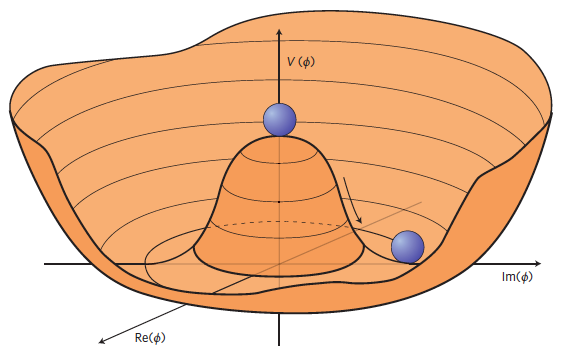
\includegraphics[width= .7\textwidth]{Figures/Introduction/higgspotential.png}
\caption[Form of the Higgs potential.]{Form of the Higgs potential giving rise to \ac{SSB} via the \ac{BEH} mechanism. Figure taken from Ref~\cite{HiggsPotential}.}
\label{Figure:Introduction_HiggsPotential}
\end{figure}

\begin{equation_pad}
    \Phi^{\dagger}\Phi = -\frac{\mu^{2}}{2\lambda} = \frac{\nu^2}{2}
\end{equation_pad}

A key constraint to achieving \ac{SSB} through the \ac{BEH} mechanism is to ensure that the photon remains massless while the other gauge bosons acquire mass. Hence, the Higgs potential's minimum must correspond to a nonzero \ac{VEV} exclusively for the neutral scalar field, $\phi^{0}$. This condition preserves the $\mathcal{U}(1)_{\text{EM}}$ symmetry after \ac{SSB}.

\begin{equation_pad}
    <0|\Phi|0> = \frac{1}{\sqrt{2}} \begin{pmatrix}
        0 \\
        \nu
    \end{pmatrix}
\end{equation_pad}
 
Before expanding the Higgs field around its minimum to study the consequences of \ac{SSB}, it is important to recall \textbf{Goldstone's theorem}~\cite{Goldstone}. \textit{This theorem predicts the emergence of a massless scalar (Goldstone) boson after the spontaneous breaking of a continuous symmetry}. Out of the four \ac{dof} introduced by the Higgs field, the three associated with the broken symmetry generators become Goldstone bosons, which appear as massless scalar fields in the Lagrangian. Gauge invariance guarantees that the choice of gauge does not affect the physical predictions of the theory, allowing us to eliminate the Goldstone bosons from the Lagrangian by making an appropriate local gauge transformation. This is referred to as the unitary gauge, where the \ac{dof} associated with the massless Goldstone bosons are replaced with new \ac{dof} corresponding to the longitudinal polarisation states of the gauge bosons ($\PW^{\pm}/\PZ$). In the unitary gauge, the Higgs field can be re-expressed as,

\begin{equation_pad}
    \text{BEH} \rightarrow \Phi = \frac{1}{\sqrt{2}}\begin{pmatrix}
        0 \\
        \nu + h
    \end{pmatrix} 
    \label{Equation:Introduction_HiggsField_2}
\end{equation_pad}

where h is the physical Higgs field, the fourth \ac{dof} in the Higgs sector.

The term in the Lagrangian responsible for the generation of the masses of gauge bosons is $(D_\mu\Phi)^\dagger(D^\mu\Phi)$. Substituting Eq.~\ref{Equation:Introduction_HiggsField_2} into this term and expressing the $B_\mu$ and $W_{\mu}^{(i)}$ fields in terms of physical $Z_\mu$ and $W_{\mu}^{\pm}$ states using Eq.~\ref{Equation:Introduction_PhysicalGaugeFields}, we obtain the following weak boson mass terms,

\begin{equation_pad}
    \text{BEH} \rightarrow \mathcal{L}_{\text{Higgs}} \supset \frac{1}{4} g^2 \nu^2 W^{+\mu}W_{\mu}^- + \frac{(g^2+g'^2)\nu^2}{8} Z_\mu Z^\mu
\label{Equation:Introduction_HiggsLagrangian_2}
\end{equation_pad}

Using the known form of a mass term for a spin-1 gauge boson, the masses of the $W^\pm$ and the Z bosons can be expressed in terms of the $\mathcal{SU}(2)_{L}$ $\otimes$ $\mathcal{U}(1)_{Y}$ gauge couplings and the Higgs \ac{VEV} ($\nu = 246 \GeV$) as,

\begin{equation_pad}
\begin{aligned}
    m_W &= \frac{1}{2}g\nu \\
    m_Z &= \frac{1}{2}\nu\sqrt{g^2+g'^2}\\
\end{aligned}
\end{equation_pad}

Importantly, in this physical basis, the neutral gauge boson associated with the $\text{A}_\mu$ field remains massless while the physical Higgs field also appears in the Lagrangian with the associated terms being,

\begin{equation_pad}
    \text{BEH} \rightarrow \mathcal{L}_{\text{Higgs}} \supset \underbrace{\frac{1}{2} \partial_\mu h \, \partial^\mu h - \lambda \nu^2 h^2}_{\text{massive scalar boson } h}
    \underbrace{- \lambda \nu h^3 - \frac{1}{4} \lambda h^4}_{\text{Higgs self-interactions}}
\label{Equation:Introduction_HiggsLagrangian_3}
\end{equation_pad}

According to Eq.~\ref{Equation:Introduction_HiggsLagrangian_3}, the mass of the scalar boson field in given by $\text{m}_H = \sqrt{2\lambda}\nu$. This Lagrangian also contains terms describing the trilinear and quartic self-interactions of the Higgs boson for which the relevant Feynman diagrams are shown in Fig.~\ref{Figure:Introduction_HiggsSelf}. While only the self-interaction terms are shown in Eq.~\ref{Equation:Introduction_HiggsLagrangian_3}, the Lagrangian also contains interaction terms between the Higgs boson and the weak gauge bosons ($\PW^\pm/\PZ$). 

\begin{figure}[h]
    \centering
    % First row
    \begin{subfigure}{0.45\textwidth}
        \centering
        \begin{tikzpicture}
    \begin{feynman}
        \vertex[blue] at (0, 0) (a) {\(H\)};
        \vertex at (2, 0) (center);
        \vertex[blue] at (4, 1.5) (b) {\(H\)};
        \vertex[blue] at (4, -1.5) (c) {\(H\)};

        \diagram*{
            (a) -- [scalar] (center),
            (center) -- [scalar] (b),
            (center) -- [scalar] (c),
        };
    \end{feynman}
\end{tikzpicture}


    \end{subfigure}
    \hfill
    \begin{subfigure}{0.45\textwidth}
        \centering
        \begin{tikzpicture}
    \begin{feynman}
        \vertex[blue] at (0, 1.5) (a) {\(H\)};
        \vertex[blue] at (0, -1.5) (a1) {\(H\)};

        \vertex at (2, 0) (center);
        \vertex[blue] at (4, 1.5) (b) {\(H\)};
        \vertex[blue] at (4, -1.5) (c) {\(H\)};

        \diagram*{
            (a) -- [scalar] (center),
            (a1) -- [scalar] (center),
            (center) -- [scalar] (b),
            (center) -- [scalar] (c),
        };
    \end{feynman}
\end{tikzpicture}


    \end{subfigure}
    \caption[Feynman diagrams from Higgs self-interactions in the Standard Model]{Feynman diagrams arising from the presence of the Higgs self-interaction terms in the \ac{SM} Lagrangian.}
    \label{Figure:Introduction_HiggsSelf}
\end{figure}

Remarkably, fermions in the \ac{SM} also acquire masses via the \ac{BEH} mechanism through Yukawa interactions. After \ac{SSB}, when the Higgs field acquires a \ac{VEV}, the Yukawa part of the Lagrangian takes the form

\begin{equation_pad}
    \text{BEH} \rightarrow \mathcal{L}_{\text{Yukawa}}^f = \underbrace{-\frac{g_f}{\sqrt{2}}\nu(\overline{\psi_L}\psi_R + \overline{\psi_R} \psi_L)}_{\text{mass term}} \underbrace{- \frac{g_f}{\sqrt{2}}h(\overline{\psi_L}\psi_R + \overline{\psi_R} \psi_L)}_{\text{interaction term}}
\label{Equation:Introduction_YukawaLagrangian}
\end{equation_pad}

where $\psi_L$ and $\psi_R$ are the left-handed and right-handed chiral fields, and the first term gives the fermionic mass $m_f = g_f\nu / \sqrt{2}$. The second term in the Lagrangian describes the coupling between the fermion and the Higgs boson itself, interestingly indicating that heavier fermions couple stronger to the Higgs.

\section{The Higgs boson}

Undoubtedly, one of the most significant achievements in modern physics is the observation of the long-sought fundamental boson, the Higgs. The confirmation of its existence came in 2012, when the ATLAS and \ac{CMS} Collaborations~\cite{Higgs_ATLAS,Higgs_CMS} jointly announced its discovery, marking the completion of the \ac{SM} particle content. Soon after its discovery, both collaborations conducted several measurements exploring the properties of the Higgs, demonstrating that the observed Higgs looks very much like the \ac{SM} Higgs~\cite{HiggsParity_1,HiggsParity_2}. One important test lies in the Higgs boson couplings. The most recent measurements of the coupling strengths~\cite{CMS_Couplings_Measurement} are consistent with the \ac{SM} prediction, as presented in Fig.~\ref{Figure:Introduction_CMScouplings}.

\begin{figure}[h]
\centering
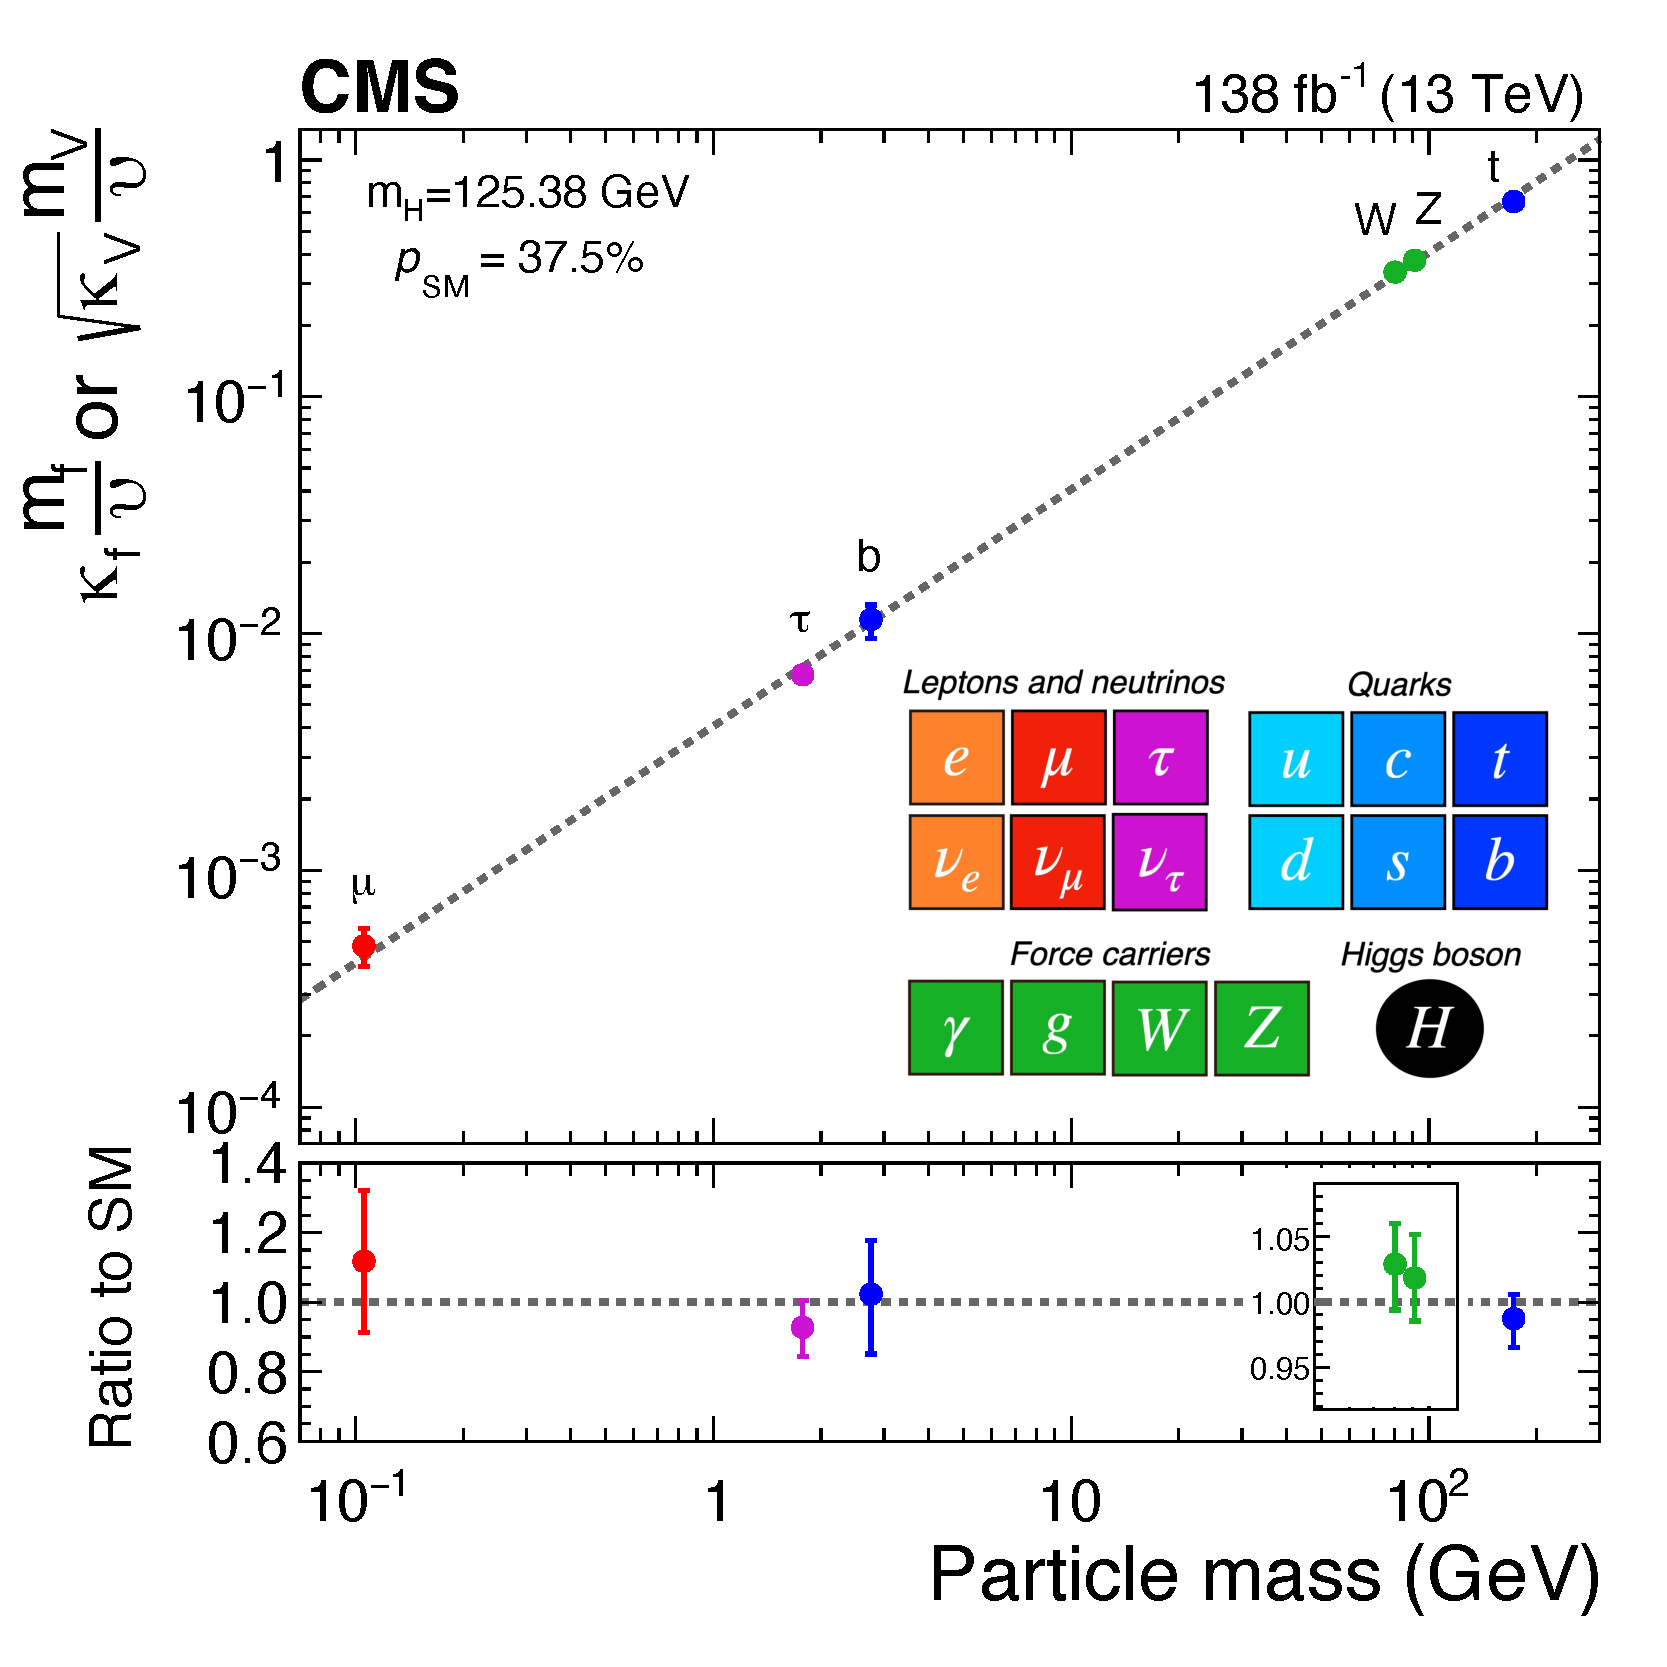
\includegraphics[width= .7\textwidth]{Figures/Introduction/CMS_Higgs_FermionCouplings.pdf}
\caption[Measured Higgs coupling modifiers versus fermion and boson masses]{The measured coupling strength modifiers of the Higgs boson to fermions and heavy gauge bosons are presented as a function of the fermionic/bosonic masses. For gauge bosons, the ``reduced" coupling modifiers are presented to keep a linear proportionality to the mass. Figure taken from Ref.~\cite{CMS_Couplings_Measurement}.}
\label{Figure:Introduction_CMScouplings}
\end{figure}

\subsection{Higgs boson production}

At the \ac{LHC}, the Higgs boson is produced via four major production modes: \textit{\ac{ggH}}, \textit{\ac{VBF}}, \textit{\ac{VH}}, and \textit{$t\overline{t}$-associated production} (ttH); listed in order of decreasing cross-section. In addition to the dominant production modes, the Higgs can still be produced in different ways \eg \textit{in association with a single-top} (tH). The Feynman diagrams of the dominant modes are displayed in Fig.~\ref{Figure:Introduction_HiggsProductionModes} while their respective cross-sections at $\sqrt{s}$ = 13$\TeV$ and $\sqrt{s}$ = 13.6$\TeV$ are displayed in Table~\ref{Table:Introduction_HiggsProduction_XS}. 


\begin{figure}[h]
    \centering
    % First row
    \begin{subfigure}{0.45\textwidth}
        \centering
        \begin{tikzpicture}
    \begin{feynman}
        \vertex at (0, 1.5) (i1) {\(g\)};
        \vertex at (0,-1.5) (i2) {\(g\)};
        \vertex at (2.5, 1.5) (a);
        \vertex at (2.5,-1.5) (b);
        \vertex at (4, 0) (c);
        \vertex[blue] at (6, 0) (f) {\(H\)};
        \vertex at (3.25,0) () {\(t\)};
        \diagram*{
            (i1) -- [gluon] (a),
            (i2) -- [gluon] (b),
            (a) -- [fermion] (b) -- [fermion] (c) -- [fermion] (a),
            (c) -- [scalar] (f),
        };
    \end{feynman}
\end{tikzpicture}


        \caption{ggH}
    \end{subfigure}
    \hfill
    \begin{subfigure}{0.45\textwidth}
        \centering
        \begin{tikzpicture}
    \begin{feynman}
        \vertex at (0, 1.) (i1) {\(q\)};
        \vertex at (0,-1.) (i2) {\(q\)};

        \vertex at (3, 1) (a);
        \vertex at (3,-1) (b);
        \vertex at (4,0) (c);

        \vertex[blue] at (6, 0) (f) {\(H\)};
        \vertex at (6, 1.5) (e) {\(q\)};
        \vertex at (6,-1.5) (g) {\(q\)};

        \vertex at (4.25,0.6) () {\(W/Z\)};
        \vertex at (4.25,-0.6) () {\(W/Z\)};

        \diagram*{
            (i1) -- [fermion] (a),
            (i2) -- [fermion] (b),
            (a) -- [photon] (c),
            (b) -- [photon] (c),
            (c) -- [scalar] (f),
            (a) -- [fermion] (e),
            (b) -- [fermion] (g),
        };
    \end{feynman}
\end{tikzpicture}
        \caption{VBF}
    \end{subfigure}

    % Add vertical space between rows
    \vspace{0.5cm}

    % Second row (centered properly)
    \begin{subfigure}{0.45\textwidth}
        \centering
        \raisebox{-5mm}{\begin{tikzpicture}
    \begin{feynman}
        \vertex at (0, 1.5) (i1) {\(q\)};
        \vertex at (0,-1.5) (i2) {\(\overline{q}\)};

        \vertex at (2,0) (a);
        \vertex at (4, 0) (b);

        \vertex at (6.15, 1.5) (c) {\(W/Z\)};
        \vertex[blue] at (6,-1.5) (d) {\(H\)};

        \vertex at (3,0.25) () {\(W/Z\)};

        \diagram*{
            (i1) -- [fermion] (a) -- [fermion] (i2),
            (a) -- [photon] (b),
            (b) -- [photon] (c),
            (b) -- [scalar] (d),
        };
    \end{feynman}
\end{tikzpicture}}
        \caption{WZ associated}
    \end{subfigure}
    \hfill
    \begin{subfigure}{0.45\textwidth}
        \centering
        \begin{tikzpicture}
    \begin{feynman}
        \vertex at (0, 1.5) (i1) {\(g\)};
        \vertex at (0,-1.5) (i2) {\(g\)};
        
        \vertex at (3, 1.5) (a);
        \vertex at (3,0) (ab);
        \vertex at (3,-1.5) (b);
        
        \vertex at (6, 1.5) (c) {\(\overline{t}\)};
        \vertex at (6, -1.5) (d) {\(t\)};

        \vertex[blue] at (6, 0) (f) {\(H\)};

        \diagram*{
            (i1) -- [gluon] (a),
            (i2) -- [gluon] (b),
            (c) -- [fermion] (a),
            (a) -- [fermion] (ab),
            (ab) -- [fermion] (b),
            (b) -- [fermion] (d),
            (ab) -- [scalar] (f),
        };
    \end{feynman}
\end{tikzpicture}


        \caption{$t\bar{t}$ associated}
    \end{subfigure}

    \caption{Feynman diagrams of the main Standard Model Higgs production modes at the Large Hadron Collider.}
    \label{Figure:Introduction_HiggsProductionModes}
\end{figure}


\begin{table}[htbp]
\centering
\renewcommand{\arraystretch}{1.5} % Increase row height
\arrayrulecolor{black} % Ensure outer border is black
\begin{tabular}{|c|c|c|}
\hline
Mechanism & Cross Section @ 13 TeV [pb] & Cross Section @ 13.6 TeV [pb] \\ \hline \hline 
ggH                                & 48.60  & 52.23 \\ 
\arrayrulecolor{lightgray} \hline
VBF                                & 3.78  & 4.08 \\ 
\arrayrulecolor{lightgray} \hline
WH                                 & 1.37  & 1.46 \\ 
\arrayrulecolor{lightgray} \hline
ZH                                 & 0.76  & 0.94 \\ 
\arrayrulecolor{lightgray} \hline
ttH                                & 0.51  & 0.57 \\ 
\arrayrulecolor{black} \hline
\end{tabular}
\caption[Cross sections of dominant Standard Model Higgs production modes at $13$ and $13.6\TeV$]{Cross sections of the dominant Higgs production mechanisms in the \ac{SM}. Derived for $\text{m}_H = 125\GeV$ and presented for both $\sqrt{s}=13\TeV$ and $\sqrt{s}=13.6\TeV$~\cite{HiggsProduction_XS_13TeV,HiggsProduction_XS_13p6TeV}.}
\label{Table:Introduction_HiggsProduction_XS}
\end{table}

The ggH production mode is the most dominant, proceeding via an internal quark loop. This is a consequence of the Higgs not directly coupling to the gluon. Despite its dominance, other production modes, such as VBF, have an interesting feature: additional objects in their final states. These distinct topologies can be leveraged to reduce backgrounds. In particular, the VBF production mode is characterised by two additional energetic jets, which tend to have a large spatial separation and a high invariant mass.

\subsection{Higgs boson decays}

The Higgs boson is an unstable particle, decaying almost immediately after its production~\cite{MarkThompson}, with its inference only possible from the decay products. The dominant \ac{SM} Higgs decays channels are listed in Table~\ref{Table:Introduction_HiggsBranchingFractions}, clearly showing that $H\rightarrow b\overline{b}$ is the dominant decay mode. 

\begin{table}[h]
\centering
\renewcommand{\arraystretch}{1.5} % Increase row height
\setlength{\tabcolsep}{12pt} % Increase column width
\arrayrulecolor{black} % Ensure outer border is black
\begin{tabular}{|c|c|}
\hline
Decay Mode                  & Branching Fraction {[}\%{]} \\ \hline \hline
$b\overline{b}$             & 58.24 \\ 
\arrayrulecolor{lightgray} \hline
$WW^*$                      & 21.37 \\ 
\arrayrulecolor{lightgray} \hline
$gg$                        & 8.19  \\ 
\arrayrulecolor{lightgray} \hline
$\tau\tau$                  & 6.27  \\ 
\arrayrulecolor{lightgray} \hline
$c\overline{c}$             & 2.89  \\ 
\arrayrulecolor{lightgray} \hline
$ZZ^*$                      & 2.61  \\ 
\arrayrulecolor{lightgray} \hline
$\gamma\gamma$              & 0.23  \\ 
\arrayrulecolor{lightgray} \hline
$\mu\mu$                    & 0.02  \\ 
\arrayrulecolor{black} \hline
\end{tabular}
\caption[Branching fractions of main Standard Model Higgs decay channels at $\text{m}_H = 125\GeV$]{Branching fractions, $\text{B}_f$, of the main \ac{SM} Higgs boson decay channel for $\text{m}_H = 125\GeV$~\cite{HiggsProduction_XS_13TeV,HiggsProduction_XS_13p6TeV} where for a particular final state $f$, $\text{B}_f = \Gamma_f/\Gamma_H$, with $\Gamma_f$ and $\Gamma_H$ being the decay width of the final state and the Higgs boson respectively.}
\label{Table:Introduction_HiggsBranchingFractions}
\end{table}

However, the sensitivity of this mode is heavily impacted by the presence of a large hadronic background. The Higgs discovery was only possible after a combination of several of the decay channels; $H\rightarrow ZZ \rightarrow 4l$, $H\rightarrow \gamma \gamma$, $H\rightarrow WW^*$, $H\rightarrow \tau\tau$ and $H\rightarrow b\overline{b}$, with the di-photon and four lepton decay channels being the main contributors. Particularly interesting is the $H\rightarrow \tau\tau$ decay mode, providing a relatively large branching fraction while being less impaired by backgrounds than $H\rightarrow b\overline{b}$.

\chapter*{Introduction }
\addcontentsline{toc}{chapter}{Introduction}

\setcounter{mtc}{1}
\chapter{The Standard Model of particle physics}
\chaptermark{The Standard Model of particle physics}  
\thispagestyle{plain}  % First page has default style
\pagestyle{chapterpages}
\label{Section:Chapter1}

\minitoc

The \ac{SM} of particle physics~\cite{Glashow_1, Weinberg_1, Salam_1, MarkThompson}\footnote{References~\cite{Glashow_1, Weinberg_1, Salam_1} correspond to the foundational works on electroweak unification, while Reference~\cite{MarkThompson} provides an accessible and comprehensive textbook overview of the entire \ac{SM}.} is our current best theoretical framework underpinning our understanding of the subatomic world. It provides a description of fundamental elementary particles and their interactions via the \textit{electromagnetic force}, \textit{weak nuclear force} and \textit{strong nuclear force}. The fourth fundamental force of nature, \textit{gravity}, is absent from the \ac{SM}, highlighting one of its key limitations. However, in high-energy physics experiments, where the interactions of subatomic particles are being studied, the omission of gravity is considered a safe simplification. Extremely powerful predictions have emerged from this theoretical framework, with its greatest accomplishments being the prediction~\cite{Englert_Brout,PeterHiggs_1,PeterHiggs_2, PeterHiggs_3, Guralnik_Hagen_Kibble, Kibble} and subsequent discovery of the \textit{Higgs boson} in 2012~\cite{Higgs_ATLAS,Higgs_CMS}. Despite its success, the \ac{SM} has its limitations. Along with the absence of gravity, it leaves several fundamental questions unanswered, such as the nature of \textit{neutrino oscillations}~\cite{Neutrino_Oscillations, Neutrino_Oscillations_2}, the existence of \textit{dark matter}~\cite{DarkMatter_1,DarkMatter_2,DarkMatter_3}\footnote{Reference~\cite{DarkMatter_1} is a modern English translation of Zwicky's seminal 1933 paper, which first proposed the concept of dark matter}, the \textit{hierarchy problem}~\cite{HierarchyProblem}, and the \textit{matter-antimatter asymmetry} in the universe~\cite{MatterAntimatter}. These have been driving the field to look for explanations beyond the \ac{SM}. In the pursuit of \ac{BSM} physics, a deep understanding of the \ac{SM} theory is crucial. The goal of this chapter is to establish the base foundation for this work, the \ac{SM}, by exploring the fundamental blocks of the theory.

\section{Particle content and fundamental interactions}
\label{Section:Particle content and fundamental interactions}
Built on the theoretical framework of \ac{QFT}, the \ac{SM} is a renormalisable theory. In this theory, the physical particles observed in nature, referred to as \textit{fermions}, emerge as quantised excitations of underlying relativistic fields. Force carriers mediate their interactions, \textit{vector bosons}, and together, these two groups of particles constitute the particle content of the \ac{SM}, as shown in Fig.~\ref{Figure:Introduction_1}.

\begin{figure}[ht]
\centering
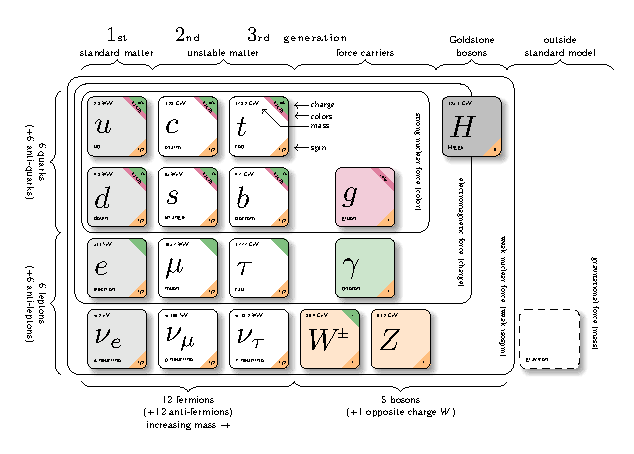
\includegraphics[width= 0.9\textwidth]{Figures/Introduction/Particles.pdf}
\caption[Diagram of the particle content of the Standard Model]{Diagram of the particle content of the \ac{SM}. For each fundamental particle, the charges, colour and spin quantum numbers are available. The measured masses for all fermions and gauge bosons are taken from Ref.~\cite{ParticleMasses} with the exception of the Higgs mass, which is taken from Ref.~\cite{Higgs_Mass}.}
\label{Figure:Introduction_1}
\end{figure}

Within the \ac{SM}, fermions serve as the fundamental constituents of all observable matter. These elementary, non-composite, spin-1/2 particles are organised into three distinct generations, with each fermion paired with an antiparticle. The antiparticles exhibit quantum numbers precisely opposite in sign, with the exception of mass and spin, which remain identical. As shown in Fig.~\ref{Figure:Introduction_1}, fermions are further divided into \textit{quarks} and \textit{leptons}. 

The leptonic sector consists of three charged leptons (\textit{electron, muon, tau}) and three electrically neutral neutrinos (\textit{electron neutrino, muon neutrino, tau neutrino}). The quark sector, on the other hand, comprises of six quark flavours; \textit{up}, \textit{down}, \textit{charm}, \textit{strange}, \textit{top} and \textit{bottom}. Within the first generation, the electron and electron neutrino comprise the leptons, while the up and down quarks form the quark sector. Although fundamental quantum numbers remain identical across generations\footnote{While fundamental quantum numbers like electric charge remain constant, others, such as flavour, vary across generations, as do properties like mass.}, the mass spectrum exhibits a strong hierarchy, with the third generation being significantly heavier than the first.

A key distinction between leptons and quarks lies in their participation in strong interactions. Unlike leptons, quarks possess an additional quantum number known as a colour charge, enabling their interactions via the strong force, which is mediated by massless gluons ($\Pg$). In addition to the strong interaction, charged leptons and quarks interact electromagnetically due to their electric charge, with massless photons ($\PGg$) acting as the mediators of the force. Conversely, neutrinos, being electrically neutral, do not participate in electromagnetic interactions. All fermions, including neutrinos, interact via the weak interaction, which occurs via the exchange of massive vector bosons, $\PW^\pm$ bosons and $\PZ$ bosons. These fundamental interactions are explored in more detail in the following section.

\section{Foundation of the fundamental interactions}
\label{Section:Chapter1_FundamentalInteractions}

Symmetries describing the fundamental interactions are the core of the \ac{SM}. N\"{o}ether's theorem~\cite{Noether_1,Noether_2}\footnote{Reference~\cite{Noether_1} is an english translation of N\"{o}ether's original paper.} shows that a conservation law is implied by the invariance of a Lagrangian under a continuous transformation (symmetry). A striking example of the deep connection between fundamental interactions and symmetry principles is the conservation of angular momentum, defined by a Lagrangian, which is invariant under rotational transformations. 

The \ac{SM} is a \textit{gauge theory} built on the principle of \textit{local gauge invariance} \ie the Lagrangian is invariant under local phase transformations. Such transformations shift the phase of the field ($\psi(x)$) as a function of the spacetime coordinates

\begin{equation_pad}
    \psi(x) \rightarrow e^{iq\theta(x)} \psi(x)
\label{Equation:Introduction_LocalPhaseTransformation}
\end{equation_pad}

where $q$ is the charge associated with the gauge symmetry and 
$\theta(x)$ is a \\ spacetime-dependent function representing the local phase transformation. The introduction of the gauge boson fields mediating fermion interactions is a direct consequence of imposing this invariance. Alone, a local phase transformation would break the invariance of the \ac{SM} Lagrangian, which is restored by the introduction of the gauge boson fields.

\subsection{Quantum Electrodynamics}
The \ac{QFT} of electromagnetism, known as \textbf{\ac{QED}}~\cite{QED}, describes the interactions between electrically charged fermions through the exchange of photons. Remarkably, the entire framework of \ac{QED} emerges beautifully from a single guiding principle: \textit{the requirement that the \ac{QED} Lagrangian remains invariant under local $\mathcal{U}$(1) gauge transformations}. The foundation of \ac{QED} begins with the Dirac equation \cite{MarkThompson} which describes the equations of motion for spin-$\frac{1}{2}$ fermion fields,

\begin{equation_pad}
    \mathcal{L}_{\text{Dirac}} = \overline{\psi}(i\gamma^\mu \partial_\mu - m_{\psi}) \psi
\label{Equation:Introduction_DiracEquation}
\end{equation_pad}

where $\psi$ and its adjoint $\overline{\psi}$ are the fermion fields expressed as four-component Dirac spinors while the quantity $\gamma^\mu$ represents the Dirac gamma matrices. Finally, $m_{\psi}$ represents the mass of the fermion.

As briefly discussed in Section~\ref{Section:Chapter1_FundamentalInteractions}, under a local $\mathcal{U}$(1) gauge transformation, the fermion field transforms in a way (Eq.~\ref{Equation:Introduction_LocalPhaseTransformation}) that breaks the local gauge invariance of the Lagrangian. Under this transformation, the Dirac equation (Eq.~\ref{Equation:Introduction_DiracEquation}) becomes

\begin{equation_pad}
    \mathcal{U}(1) \rightarrow \mathcal{L}_{\text{Dirac}}^{\prime} = \mathcal{L}_{\text{Dirac}} - q\overline{\psi}\gamma^\mu(\partial_\mu\theta(x))\psi
\label{Equation:Introduction_Dirac(U1)}
\end{equation_pad}

To restore local gauge invariance, the derivative $\partial_\mu$ is replaced with the covariant derivative $D_\mu$,

\begin{equation_pad}
    \partial_\mu \rightarrow D_\mu = \partial_\mu + iqA_\mu
\end{equation_pad}

where $A_\mu$ is a new field. The problematic term in Eq.\ref{Equation:Introduction_Dirac(U1)} can be cancelled out provided that the new field transforms as

\begin{equation_pad}
    \mathcal{U}(1) \rightarrow A_\mu^{\prime} = A_\mu - \partial_\mu \theta(x) 
\end{equation_pad}

Therefore, imposing a $\mathcal{U}$(1) local gauge invariance on the Lagrangian has forced the existence of a photon field, $A_\mu$, with well-defined gauge transformation properties. The local gauge-invariant Lagrangian for a spin-1/2 fermion field becomes

\begin{equation_pad}
    \mathcal{L}_{\text{Dirac}} = \overline{\psi}(i\gamma^\mu \partial_\mu - m_{\psi}) \psi - q\overline{\psi}\gamma^\mu A_\mu\psi
\label{Equation:Dirac_GaugeInvariant}
\end{equation_pad}

The additional term in the Lagrangian (Eq.\ref{Equation:Dirac_GaugeInvariant}) encapsulates the electromagnetic interaction between charged fermions and photons. The strength of this coupling is given by $q = |e|Q$, where e denotes the fundamental unit of electric charge, and Q represents the dimensionless charge of the fermion field $\psi$ relative to e. By N\"{o}ether's theorem, electric charge corresponds to the conserved quantity associated with a local $\mathcal{U}$(1) gauge symmetry, once again reinforcing the deep connection between symmetry and conservation laws in \ac{QFT}. The final component necessary to complete the \ac{QED} Lagrangian is the gauge-invariant kinetic term for the massless spin-1 field, described by the field strength tensor $F_{\mu\nu}$. Incorporating this, the total \ac{QED} Lagrangian takes the form,

\begin{equation_pad}
    \mathcal{L}_{\text{QED}} = \overline{\psi}(i\gamma^\mu \partial_\mu - m_{\psi}) \psi - q\overline{\psi}\gamma^\mu A_\mu\psi - \frac{1}{4}F_{\mu\nu}F^{\mu\nu}
\label{Equation:QED_GaugeInvariant}
\end{equation_pad}

\begin{equation_pad}
F_{\mu\nu} = \partial_\mu A_\nu - \partial_\nu A_\mu
\end{equation_pad}

\subsection{Quantum Chromodynamics}

The \ac{QFT} describing the strong interaction is known as \textbf{\ac{QCD}}. \ac{QCD} governs the dynamics of quarks and gluons, and \textit{it is formulated as a non-Abelian gauge theory under the local $\mathcal{SU}(3)_C$ symmetry group}. While \ac{QED} applies universally to all charged particles, the gauge symmetry of \ac{QCD} only applies to fields that carry colour charge, as denoted by the subscript $C$.

Unlike the Abelian $\mathcal{U}$(1) symmetry of \ac{QED}, which involves a single generator, the $\mathcal{SU}(3)$ symmetry group is represented by eight generators, $T^a$. To ensure local $\mathcal{SU}(3)_C$ gauge invariance, the derivative $\partial_\mu$ is replaced with the covariant derivative expressed in terms of the generators as

\begin{equation_pad}
    \partial_\mu \rightarrow D_\mu = \partial_\mu + ig_sG^{a}_{\mu}T^{a}
\end{equation_pad}

where $G^{a}_{\mu}$ represent the eight new fields, which correspond to the eight massless gluons mediating the strong interaction. The term $g_s$ encodes the coupling strength of the interaction. The full \ac{QCD} Lagrangian can then be expressed as

\begin{equation_pad} 
\mathcal{L}_{\text{QCD}} = \sum_{f}\overline{\psi_f}(i\gamma^\mu D_\mu - m_f)\psi_f - \frac{1}{4} G^{\mu\nu}_{a}G^{a}_{\mu\nu}
\end{equation_pad}

where $\psi_f$ represents the quark field (spinor) for the $f^{th}$ flavour. Once again, according to N\"{o}ether's theorem, colour charge corresponds to the conserved quantity associated with local $\mathcal{SU}(3)_C$ gauge symmetry.

Unlike \ac{QED}, the kinetic (gauge term) in the Lagrangian includes additional terms representing the self-interactions of the gauge bosons. This is a direct consequence of the \ac{QCD} generators not commuting,

\begin{equation_pad}
    [T^a,T^b] = if^{abc}T^c
\end{equation_pad}

which allows gluons themselves to carry colour charge. The quantity $f^{abc}$ refers to the structure constants of the symmetry group. This gluon self-interaction property modifies the strength of the interaction ($\alpha_{S}$), causing it to decrease as a function of the interaction energy scale. Hence, $\alpha_{S}$ is referred to as a running coupling constant.

An important consequence of this is \textit{asymptotic freedom}~\cite{AsymptoticFreedom_1,AsymptoticFreedom_2}, where at very high energies (short distances), such as the deep scattering energies at the \ac{LHC}, $\alpha_{S}$ decreases approaching zero. In this scenario, quarks and gluons behave as quasi-free particles within the protons and neutrons, allowing perturbative \ac{QCD} to describe their interactions accurately. However, at low energies, the strong coupling grows large, making \ac{QCD} non-perturbative. In this regime, quarks and gluons are not found as free particles but instead form bound, colour-neutral states known as hadrons. This phenomenon, known as \textit{colour confinement}~\cite{MarkThompson}\footnote{The phenomenon of colour confinement was first motivated theoretically in the 1970s through ideas such as flux tube formation and asymptotic freedom. A clear summary is provided in Reference~\cite{MarkThompson}.}, ensures that isolated colour-charged particles do not exist in nature; only hadrons are observed.

As a consequence of colour confinement, in high-energy collisions, high-energy quarks and gluons are observed as jets~\cite{Hadronisation_Jets} of colourless particles formed through a process known as hadronisation. In the context of proton-proton (pp) collisions, highly energetic partons fly away from the interaction point. As the partons separate, the colour field between them can be thought of as if it is being squeezed in a tube, with the energy in the field becoming increasingly larger with distance. Once that energy becomes sufficient, a new quark-antiquark pair is produced, separating the colour field into smaller segments. Eventually, the formation of colourless hadrons occurs when the quark-antiquark pairs have sufficiently low energy. This resulting cascade of collimated hadrons forms what is observed as a jet. A qualitative schematic of the hadronisation process is shown in Fig.~\ref{Figure:Introduction_ColourConfinement}.

\begin{figure}[h]
    \centering
    \begin{tikzpicture}[>=stealth,thick]

%----------------- (i) -----------------%
\node at (-2,0) {\large (i)};
% Quark & antiquark with arrows
\node[circle, fill=black, scale=0.7, label=above:$q$] (q_i) at (4.5,0) {};
\node[circle, fill=black, scale=0.7, label=above:$\bar{q}$] (qb_i) at (5.5,0) {};
\draw[->] (q_i) -- ++(-1.5, 0);
\draw[->] (qb_i) -- ++(+1.5, 0);

%----------------- (ii) -----------------%
\node at (-2,-1.5) {\large (ii)};
% Another q/qbar pair with a flux tube (string)
\node[circle, fill=black, scale=0.7, label=above:$q$] (q_ii) at (3.5,-1.5) {};
\node[circle, fill=black, scale=0.7, label=above:$\bar{q}$] (qb_ii) at (6.5,-1.5) {};
% Draw the string (solid line) plus double arrow to suggest tension
\draw[thick] (q_ii) to[out=20, in=160] (qb_ii);
\draw[thick] (q_ii) to[out=-20, in=-160] (qb_ii);
\draw (q_ii) -- (qb_ii);
\draw[->] (q_ii) -- ++(-1.5, 0);
\draw[->] (qb_ii) -- ++(+1.5, 0);

%----------------- (iii) -----------------%
\node at (-2,-3.0) {\large (iii)};
% Multiple q/qbar pairs horizontally
\node[circle, fill=black, scale=0.7, label=above:$q$] (q1_iii)  at (2.5, -3.0) {};
\node[circle, fill=black, scale=0.7, label=above:$\bar{q}$] (qb1_iii) at (4.5, -3.0) {};
\node[circle, fill=black, scale=0.7, label=above:$q$] (q2_iii)  at (5.5, -3.0) {};
\node[circle, fill=black, scale=0.7, label=above:$\bar{q}$] (qb2_iii)at (7.5, -3.0) {};

\draw[thick] (q1_iii) to[out=20, in=160] (qb1_iii);
\draw[thick] (q1_iii) to[out=-20, in=-160] (qb1_iii);
\draw[thick] (q2_iii) to[out=20, in=160] (qb2_iii);
\draw[thick] (q2_iii) to[out=-20, in=-160] (qb2_iii);

\draw (q1_iii) -- (qb1_iii);
\draw (q2_iii) -- (qb2_iii);

\draw[->] (q1_iii) -- ++(-1.5, 0);
\draw[->] (qb2_iii) -- ++(+1.5, 0);

%----------------- (iv) -----------------%
\node at (-2,-4.5) {\large (iii)};
% Multiple q/qbar pairs horizontally
\node[circle, fill=black, scale=0.7] (q11_iv)  at (1.5, -4.5) {};
\node[circle, fill=black, scale=0.7] (qb11_iv) at (2.5, -4.5) {};
\node[circle, fill=black, scale=0.7] (q12_iv)  at (3, -4.5) {};
\node[circle, fill=black, scale=0.7] (qb12_iv) at (4, -4.5) {};

\node[circle, fill=black, scale=0.7] (q21_iv)  at (5.5, -4.5) {};
\node[circle, fill=black, scale=0.7] (qb21_iv)at (6.5, -4.5) {};
\node[circle, fill=black, scale=0.7] (q22_iv)  at (7, -4.5) {};
\node[circle, fill=black, scale=0.7] (qb22_iv)at (8, -4.5) {};

\draw[thick] (q11_iv) to[out=20, in=160] (qb11_iv);
\draw[thick] (q11_iv) to[out=-20, in=-160] (qb11_iv);
\draw[thick] (q12_iv) to[out=20, in=160] (qb12_iv);
\draw[thick] (q12_iv) to[out=-20, in=-160] (qb12_iv);

\draw[thick] (q21_iv) to[out=20, in=160] (qb21_iv);
\draw[thick] (q21_iv) to[out=-20, in=-160] (qb21_iv);
\draw[thick] (q22_iv) to[out=20, in=160] (qb22_iv);
\draw[thick] (q22_iv) to[out=-20, in=-160] (qb22_iv);

\draw (q11_iv) -- (qb11_iv);
\draw (q12_iv) -- (qb12_iv);
\draw (q21_iv) -- (qb21_iv);
\draw (q22_iv) -- (qb22_iv);

\draw[->] (q11_iv) -- ++(-1.5, 0);
\draw[->] (qb22_iv) -- ++(+1.5, 0);
%----------------- (v) -----------------%
\node at (-2,-6.5) {\large (v)};
% Final hadrons on the left
\node[draw, circle, scale=1.0] (H1_v) at (1.5,-6) {};
\node[draw, circle, scale=1.0] (H2_v) at (1.7,-7) {};
\node[draw, circle, scale=1.0] (H3_v) at (2.5,-6.2) {};
\node[draw, circle, scale=1.0] (H4_v) at (2,-6.4) {};

% Arrows indicating motion outward
\draw[->] (1.2,-6) -- ++(-0.7, 0.6);
\draw[->] (1.2,-6.2) -- ++(-0.7, 0.4);
\draw[->] (1.2,-6.4) -- ++(-0.7, 0.2);
\draw[->] (1.2,-6.6) -- ++(-0.7, -0.2);
\draw[->] (1.2,-6.8) -- ++(-0.7, -0.4);
\draw[->] (1.2,-7) -- ++(-0.7, -0.6);

% Final hadrons on the right
\node[draw, circle, scale=1.0] (H5_v) at (8,-6) {};
\node[draw, circle, scale=1.0] (H6_v) at (7.8,-7) {};
\node[draw, circle, scale=1.0] (H7_v) at (7,-6.2) {};
\node[draw, circle, scale=1.0] (H8_v) at (7.5,-6.4) {};
\draw[->] (8.3,-6) -- ++(0.7, 0.6);
\draw[->] (8.3,-6.2) -- ++(0.7, 0.4);
\draw[->] (8.3,-6.4) -- ++(0.7, 0.2);
\draw[->] (8.3,-6.6) -- ++(0.7, -0.2);
\draw[->] (8.3,-6.8) -- ++(0.7, -0.4);
\draw[->] (8.3,-7) -- ++(0.7, -0.6);

\end{tikzpicture}
    \caption{Qualitative schematic of the steps involved in the hadronisation process.}
    \label{Figure:Introduction_ColourConfinement}
\end{figure}

\subsection{Electroweak theory}

In the 1960s, Glashow~\cite{Glashow_1}, Salam~\cite{Salam_1} and Weinberg~\cite{Weinberg_1} discovered that \textit{a unified picture of the electromagnetic and weak interactions} could be constructed. They proposed to develop the electroweak theory incorporating the characteristics of both interactions by associating them with the $\mathcal{SU}(2)_{L}$ $\otimes$ $\mathcal{U}(1)_{Y}$ symmetry group,

\begin{equation_pad}
    \mathcal{SU}(2)_L \otimes \mathcal{U}(1)_Y \rightarrow \mathcal{L}^{\prime}_{\text{EW}} = \mathcal{L}_{\text{EW}}
\end{equation_pad}

where $L$ denotes the \textit{left-handed nature} of the weak interaction under $\mathcal{SU}(2)_L$, and $Y$ represents the \textit{weak hypercharge} associated with the $\mathcal{U}(1)_Y$ gauge symmetry. To ensure that the electroweak Lagrangian is invariant under local transformations of this symmetry group, the covariant derivative is written as

\begin{equation_pad}
    D_\mu = \partial_\mu + \underbrace{ig^{\prime}B_\mu Y}_{\mathcal{U}(1)_Y} + \underbrace{\frac{i}{2}gW^i_\mu\sigma^i}_{\mathcal{SU}(2)_L}
\end{equation_pad}

where $Y$ is the single generator of the $\mathcal{U}(1)_Y$ gauge group, associated with the gauge boson field, $B_\mu$. While the three generators of $\mathcal{SU}(2)_L$ are represented by the 2 x 2 Pauli-spin matrices ($\sigma^i$), associated with the three gauge boson fields, $W^i_\mu$. The coupling strengths of the interactions are represented by $g$ and $g^{\prime}$, respectively. The conserved charges corresponding to these gauge symmetries are the weak isospin component, $I_3$, for $\mathcal{SU}(2)_L$ and the weak hypercharge, Y, for $\mathcal{U}(1)_Y$.

By imposing gauge invariance under the electroweak symmetry group, four gauge fields arise: the three weak isospin fields, $W_{\mu}^{(i)}$ (i=1,2,3), and the weak hypercharge field, $B_{\mu}$. These gauge fields can be expressed in terms of the physical bosons as,

\begin{equation_pad}
\begin{array}{c}
A_{\mu} = + B_{\mu} \cos{\theta_{W}} + W_{\mu}^{(3)} \sin{\theta_{W}}, \\
Z_{\mu} = - B_{\mu} \sin{\theta_{W}} + W_{\mu}^{(3)} \cos{\theta_{W}}, \\
W_{\mu}^{\pm} = \frac{1}{\sqrt{2}} (W_{\mu}^{(1)} \mp iW_{\mu}^{(2)}),
\end{array}
\label{Equation:Introduction_PhysicalGaugeFields}
\end{equation_pad}

where $\theta_{W}$, the weak mixing angle, quantifies the mixing between the weak isospin and hypercharge gauge fields. It is related to the weak and electromagnetic coupling constants, $g$ and $g^{\prime}$, by

\begin{equation_pad}
    \theta_W = \text{arctan}(\frac{g^{\prime}}{g})
\end{equation_pad}

As discussed earlier in Section~\ref{Section:Particle content and fundamental interactions}, all fermions interact via the weak interaction. A key feature of the weak interaction is its violation of parity symmetry~\cite{ParityViolation_Wu}. This means that weak interactions exhibit different behaviours under spatial inversions. In contrast to \ac{QED} and \ac{QCD}, which conserve parity and involve pure vector interactions of the form,

\begin{equation_pad}
    j^\mu = \overline{u}\gamma^\mu u
\end{equation_pad}

the weak interaction is required to take a different form to account for its parity-violating nature.

Mathematically, the proper parity transformations can be achieved by requiring the interaction to have a chiral structure. Naturally, this leads to either a V-A or V+A (Vector, Axial Vector) current. Experimentally, it is well established that the weak interaction exhibits a V-A charged current of the form,

\begin{equation_pad}
    j^\mu_{\text{weak}} = \overline{u}\gamma^\mu \frac{1}{2}(1-\gamma^5)u
\label{Equation:Chapter1-WeakChargedCurrent}
\end{equation_pad}

Using chiral operators, $P_{L/R}$, the fermion spinor fields ($u$) can be decomposed into left-handed ($u_{L}$) and right-handed ($u_{R}$) chiral components. 

\begin{equation_pad}
\begin{array}{c}
    P_{L/R} = \frac{1}{2}(1\mp \gamma^5) \quad ,\quad \gamma^5 = \gamma^0\gamma^1\gamma^2\gamma^3 \\
    u = P_Ru +P_Lu = u_R + u_L
\end{array}
\end{equation_pad}

This chiral decomposition is fundamental in the EW theory, only allowing interactions between left-handed fermions (and equivalently, right-handed anti-fermions) and the weak isospin gauge bosons $W_{\mu}^{(i)}$. This can be explicitly seen by substituting the decomposed spinor field ($u$) into the weak charged current (Eq.~\ref{Equation:Chapter1-WeakChargedCurrent}),

\begin{equation_pad}
\begin{array}{c}
    j^\mu_{\text{weak}} = (\overline{u_R} + \overline{u_L})\gamma^\mu P_L (u_R+u_L) \\
    P_L u_R = 0
\label{Equation:Chapter1-WeakChargedCurrent_Decomposed}
\end{array}
\end{equation_pad}

Hence, in this representation, it is natural that the left-handed components of the fermion fields transform as doublets under $\mathcal{SU}(2)_L$. Conversely, the right-handed components transform as singlets and do not interact with the charged weak gauge bosons. This structure of the EW theory leads to a relationship between the weak isospin, weak hypercharge and electric charge.

\begin{equation_pad}
    Q = I_3 + \frac{Y}{2}
\end{equation_pad}

where this equation beautifully encapsulates how the EW symmetry unifies the electromagnetic and weak interactions, allowing for a calculation of the charge of all fundamental particles.

Despite beautifully unifying the electromagnetic and weak interactions into a single theory, a fundamental issue persists because of non-zero mass measurements of the $\PW$ and $\PZ$ bosons~\cite{W_Z_MassMeasurements_1,W_Z_MassMeasurements_2}. This is clearly omitted from the EW Lagrangian, as including the required terms would break the underlying gauge symmetry. Mass terms of the form ${m_{W}^2 W_{\mu}^{-} W^{+\mu}}$ and $\frac{1}{2} m_{Z}^{2} Z_{\mu} Z^{\mu}$ are not invariant under the $\mathcal{SU(2)}_{L}$ $\otimes$ $\mathcal{U}(1)_{Y}$ symmetry group. This also extends to fermions with mass terms of the form, $m\overline{\psi}\psi = m(\overline{\psi}_{R}\psi_{L} + \overline{\psi}_{L}\psi_{R})$. The inclusion of such a term in the EW Lagrangian would break the symmetry because of left-handed and right-handed chiral components transform differently. The answer to this puzzle came through the Higgs mechanism, which is discussed in Section~\ref{Section:Introduction_HiggsMechanism}.

\section{Brout-Englert-Higgs mechanism}
\label{Section:Introduction_HiggsMechanism}
First proposed back in the 1960s by Englert and Brout~\cite{Englert_Brout}, Higgs~\cite{PeterHiggs_1,PeterHiggs_2,PeterHiggs_3}, and Guralnik, Hagen and Kibble~\cite{Guralnik_Hagen_Kibble,Kibble}, the \textbf{\ac{BEH} mechanism} provides a way to generate mass while preserving the local gauge invariance of the \ac{SM}. It is based on the principle of \textbf{\ac{SSB}}~\cite{SSB_Definition} where \textit{the Lagrangian of a system remains invariant under a certain symmetry group, but the vacuum state of the system does not}. The symmetry of the \ac{SM} Lagrangian is broken through the \ac{BEH} mechanism as

\begin{equation_pad}
    \mathcal{SU}(3)_C \otimes \mathcal{SU}(2)_L \otimes \mathcal{U}(1)_Y \quad \underbrace{\rightarrow}_{\text{BEH}} \quad \mathcal{SU}(3)_C \otimes \mathcal{U}(1)_{\text{EM}}
\end{equation_pad}

Effectively, the \ac{BEH} mechanism targets and breaks the symmetry of the electroweak interaction. This symmetry is broken by introducing two complex scalar fields, $\phi^{+/0}$, which transform as a doublet $\Phi$ under $SU(2)_L$ transformations,

\begin{equation_pad}
\Phi =
\begin{pmatrix}
\phi^{+} \\
\phi^{0} 
\end{pmatrix}
= \frac{1}{\sqrt{2}} \begin{pmatrix}
    \phi_{1} + i\phi_{2} \\
    \phi_{3} + i\phi_{4}
\end{pmatrix}
\end{equation_pad}

This doublet, known as the Higgs field, contributes four \ac{dof} to the \ac{SM} Lagrangian; one for the real part and one for the imaginary part of each component. The corresponding Lagrangian for the Higgs field is

\begin{equation_pad}
    \mathcal{L}_{\text{Higgs}} = (D_{\mu} \Phi)^{\dagger}(D^{\mu}\Phi) - \underbrace{(\mu^{2}\Phi^{\dagger}\Phi + \lambda(\Phi^{\dagger}\Phi)^2)}_{\text{V($\Phi$)}}
\label{Equation:Introduction_HiggsLagrangian}
\end{equation_pad}

where $D_{\mu}$ is the covariant derivative,

\begin{equation_pad}
    D_{\mu} = \partial_{\mu} + i\frac{g}{2}\vec{T}\cdot\vec{W_{\mu}} + i\frac{g'}{2}YB_{\mu}
\end{equation_pad}

The second term in Eq.~\ref{Equation:Introduction_HiggsLagrangian} represents the Higgs potential shown in Fig.~\ref{Figure:Introduction_HiggsPotential}, which depends on the Higgs field and two real parameters, $\mu^{2}$ and $\lambda$. The vacuum state of the Higgs field corresponds to the minimum of this potential, imposing constraints on these parameters. To ensure a finite minimum, $\lambda$ must be positive ($\lambda > 0$), but no such restriction applies to $\mu^{2}$. For $\mu^{2} > 0$, the potential has a single symmetric minimum at zero \ac{VEV}. Conversely, for $\mu^{2} < 0$, the potential develops an infinite set of minima, leading to \ac{SSB}  via the \ac{BEH} mechanism. In this case, the Higgs field satisfies,

\begin{figure}[h]
\centering
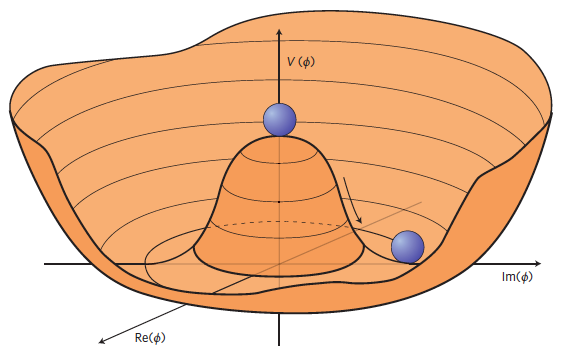
\includegraphics[width= .7\textwidth]{Figures/Introduction/higgspotential.png}
\caption[Form of the Higgs potential.]{Form of the Higgs potential giving rise to \ac{SSB} via the \ac{BEH} mechanism. Figure taken from Ref~\cite{HiggsPotential}.}
\label{Figure:Introduction_HiggsPotential}
\end{figure}

\begin{equation_pad}
    \Phi^{\dagger}\Phi = -\frac{\mu^{2}}{2\lambda} = \frac{\nu^2}{2}
\end{equation_pad}

A key constraint to achieving \ac{SSB} through the \ac{BEH} mechanism is to ensure that the photon remains massless while the other gauge bosons acquire mass. Hence, the Higgs potential's minimum must correspond to a nonzero \ac{VEV} exclusively for the neutral scalar field, $\phi^{0}$. This condition preserves the $\mathcal{U}(1)_{\text{EM}}$ symmetry after \ac{SSB}.

\begin{equation_pad}
    <0|\Phi|0> = \frac{1}{\sqrt{2}} \begin{pmatrix}
        0 \\
        \nu
    \end{pmatrix}
\end{equation_pad}
 
Before expanding the Higgs field around its minimum to study the consequences of \ac{SSB}, it is important to recall \textbf{Goldstone's theorem}~\cite{Goldstone}. \textit{This theorem predicts the emergence of a massless scalar (Goldstone) boson after the spontaneous breaking of a continuous symmetry}. Out of the four \ac{dof} introduced by the Higgs field, the three associated with the broken symmetry generators become Goldstone bosons, which appear as massless scalar fields in the Lagrangian. Gauge invariance guarantees that the choice of gauge does not affect the physical predictions of the theory, allowing us to eliminate the Goldstone bosons from the Lagrangian by making an appropriate local gauge transformation. This is referred to as the unitary gauge, where the \ac{dof} associated with the massless Goldstone bosons are replaced with new \ac{dof} corresponding to the longitudinal polarisation states of the gauge bosons ($\PW^{\pm}/\PZ$). In the unitary gauge, the Higgs field can be re-expressed as,

\begin{equation_pad}
    \text{BEH} \rightarrow \Phi = \frac{1}{\sqrt{2}}\begin{pmatrix}
        0 \\
        \nu + h
    \end{pmatrix} 
    \label{Equation:Introduction_HiggsField_2}
\end{equation_pad}

where h is the physical Higgs field, the fourth \ac{dof} in the Higgs sector.

The term in the Lagrangian responsible for the generation of the masses of gauge bosons is $(D_\mu\Phi)^\dagger(D^\mu\Phi)$. Substituting Eq.~\ref{Equation:Introduction_HiggsField_2} into this term and expressing the $B_\mu$ and $W_{\mu}^{(i)}$ fields in terms of physical $Z_\mu$ and $W_{\mu}^{\pm}$ states using Eq.~\ref{Equation:Introduction_PhysicalGaugeFields}, we obtain the following weak boson mass terms,

\begin{equation_pad}
    \text{BEH} \rightarrow \mathcal{L}_{\text{Higgs}} \supset \frac{1}{4} g^2 \nu^2 W^{+\mu}W_{\mu}^- + \frac{(g^2+g'^2)\nu^2}{8} Z_\mu Z^\mu
\label{Equation:Introduction_HiggsLagrangian_2}
\end{equation_pad}

Using the known form of a mass term for a spin-1 gauge boson, the masses of the $W^\pm$ and the Z bosons can be expressed in terms of the $\mathcal{SU}(2)_{L}$ $\otimes$ $\mathcal{U}(1)_{Y}$ gauge couplings and the Higgs \ac{VEV} ($\nu = 246 \GeV$) as,

\begin{equation_pad}
\begin{aligned}
    m_W &= \frac{1}{2}g\nu \\
    m_Z &= \frac{1}{2}\nu\sqrt{g^2+g'^2}\\
\end{aligned}
\end{equation_pad}

Importantly, in this physical basis, the neutral gauge boson associated with the $\text{A}_\mu$ field remains massless while the physical Higgs field also appears in the Lagrangian with the associated terms being,

\begin{equation_pad}
    \text{BEH} \rightarrow \mathcal{L}_{\text{Higgs}} \supset \underbrace{\frac{1}{2} \partial_\mu h \, \partial^\mu h - \lambda \nu^2 h^2}_{\text{massive scalar boson } h}
    \underbrace{- \lambda \nu h^3 - \frac{1}{4} \lambda h^4}_{\text{Higgs self-interactions}}
\label{Equation:Introduction_HiggsLagrangian_3}
\end{equation_pad}

According to Eq.~\ref{Equation:Introduction_HiggsLagrangian_3}, the mass of the scalar boson field in given by $\text{m}_H = \sqrt{2\lambda}\nu$. This Lagrangian also contains terms describing the trilinear and quartic self-interactions of the Higgs boson for which the relevant Feynman diagrams are shown in Fig.~\ref{Figure:Introduction_HiggsSelf}. While only the self-interaction terms are shown in Eq.~\ref{Equation:Introduction_HiggsLagrangian_3}, the Lagrangian also contains interaction terms between the Higgs boson and the weak gauge bosons ($\PW^\pm/\PZ$). 

\begin{figure}[h]
    \centering
    % First row
    \begin{subfigure}{0.45\textwidth}
        \centering
        \begin{tikzpicture}
    \begin{feynman}
        \vertex[blue] at (0, 0) (a) {\(H\)};
        \vertex at (2, 0) (center);
        \vertex[blue] at (4, 1.5) (b) {\(H\)};
        \vertex[blue] at (4, -1.5) (c) {\(H\)};

        \diagram*{
            (a) -- [scalar] (center),
            (center) -- [scalar] (b),
            (center) -- [scalar] (c),
        };
    \end{feynman}
\end{tikzpicture}


    \end{subfigure}
    \hfill
    \begin{subfigure}{0.45\textwidth}
        \centering
        \begin{tikzpicture}
    \begin{feynman}
        \vertex[blue] at (0, 1.5) (a) {\(H\)};
        \vertex[blue] at (0, -1.5) (a1) {\(H\)};

        \vertex at (2, 0) (center);
        \vertex[blue] at (4, 1.5) (b) {\(H\)};
        \vertex[blue] at (4, -1.5) (c) {\(H\)};

        \diagram*{
            (a) -- [scalar] (center),
            (a1) -- [scalar] (center),
            (center) -- [scalar] (b),
            (center) -- [scalar] (c),
        };
    \end{feynman}
\end{tikzpicture}


    \end{subfigure}
    \caption[Feynman diagrams from Higgs self-interactions in the Standard Model]{Feynman diagrams arising from the presence of the Higgs self-interaction terms in the \ac{SM} Lagrangian.}
    \label{Figure:Introduction_HiggsSelf}
\end{figure}

Remarkably, fermions in the \ac{SM} also acquire masses via the \ac{BEH} mechanism through Yukawa interactions. After \ac{SSB}, when the Higgs field acquires a \ac{VEV}, the Yukawa part of the Lagrangian takes the form

\begin{equation_pad}
    \text{BEH} \rightarrow \mathcal{L}_{\text{Yukawa}}^f = \underbrace{-\frac{g_f}{\sqrt{2}}\nu(\overline{\psi_L}\psi_R + \overline{\psi_R} \psi_L)}_{\text{mass term}} \underbrace{- \frac{g_f}{\sqrt{2}}h(\overline{\psi_L}\psi_R + \overline{\psi_R} \psi_L)}_{\text{interaction term}}
\label{Equation:Introduction_YukawaLagrangian}
\end{equation_pad}

where $\psi_L$ and $\psi_R$ are the left-handed and right-handed chiral fields, and the first term gives the fermionic mass $m_f = g_f\nu / \sqrt{2}$. The second term in the Lagrangian describes the coupling between the fermion and the Higgs boson itself, interestingly indicating that heavier fermions couple stronger to the Higgs.

\section{The Higgs boson}

Undoubtedly, one of the most significant achievements in modern physics is the observation of the long-sought fundamental boson, the Higgs. The confirmation of its existence came in 2012, when the ATLAS and \ac{CMS} Collaborations~\cite{Higgs_ATLAS,Higgs_CMS} jointly announced its discovery, marking the completion of the \ac{SM} particle content. Soon after its discovery, both collaborations conducted several measurements exploring the properties of the Higgs, demonstrating that the observed Higgs looks very much like the \ac{SM} Higgs~\cite{HiggsParity_1,HiggsParity_2}. One important test lies in the Higgs boson couplings. The most recent measurements of the coupling strengths~\cite{CMS_Couplings_Measurement} are consistent with the \ac{SM} prediction, as presented in Fig.~\ref{Figure:Introduction_CMScouplings}.

\begin{figure}[h]
\centering
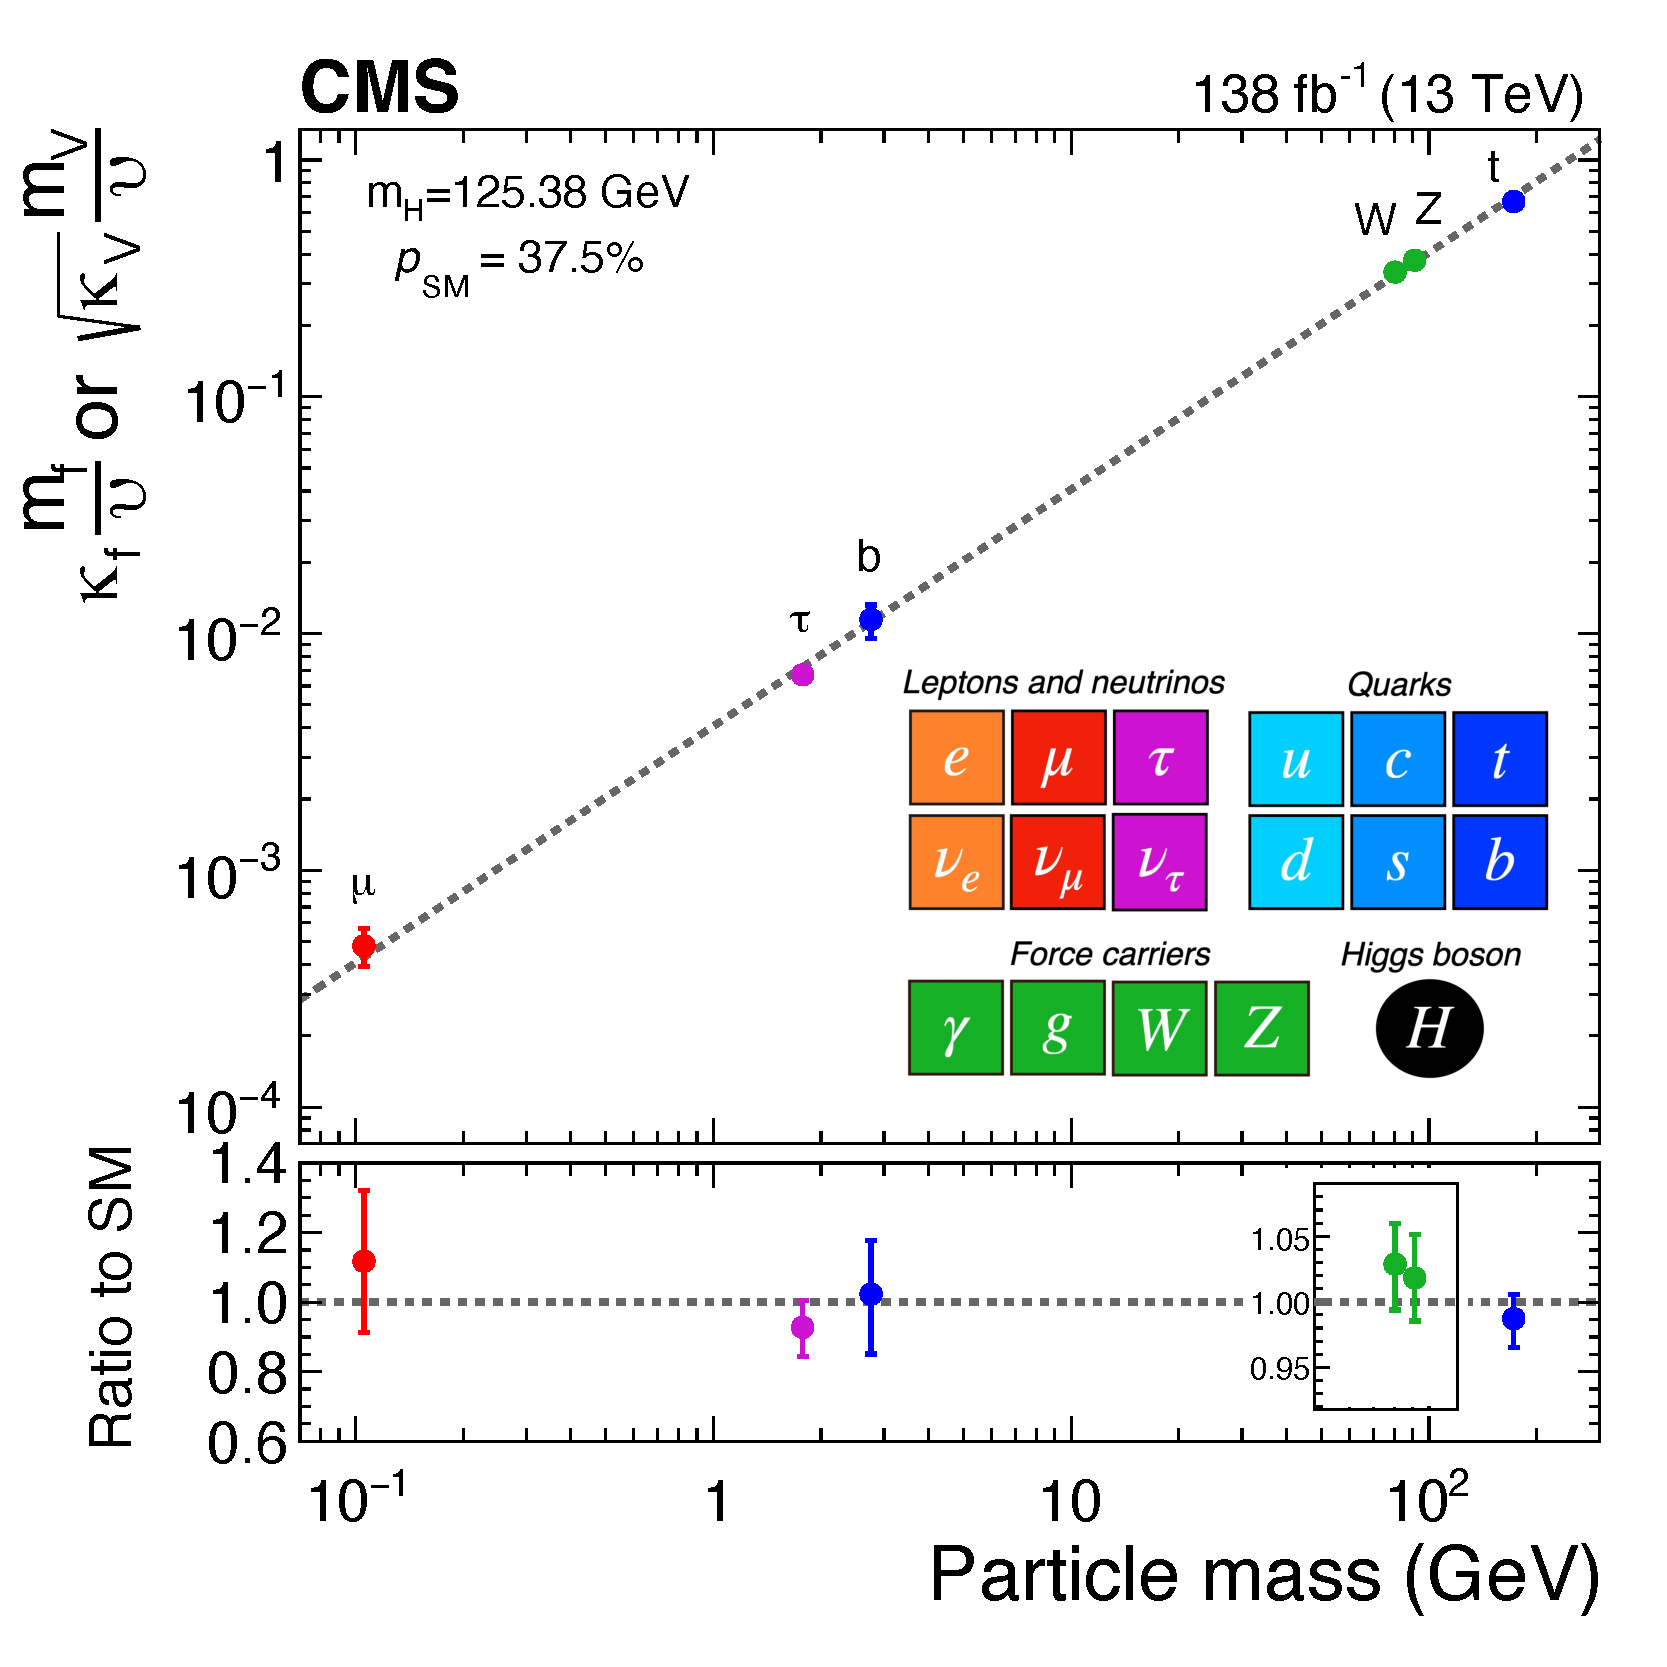
\includegraphics[width= .7\textwidth]{Figures/Introduction/CMS_Higgs_FermionCouplings.pdf}
\caption[Measured Higgs coupling modifiers versus fermion and boson masses]{The measured coupling strength modifiers of the Higgs boson to fermions and heavy gauge bosons are presented as a function of the fermionic/bosonic masses. For gauge bosons, the ``reduced" coupling modifiers are presented to keep a linear proportionality to the mass. Figure taken from Ref.~\cite{CMS_Couplings_Measurement}.}
\label{Figure:Introduction_CMScouplings}
\end{figure}

\subsection{Higgs boson production}

At the \ac{LHC}, the Higgs boson is produced via four major production modes: \textit{\ac{ggH}}, \textit{\ac{VBF}}, \textit{\ac{VH}}, and \textit{$t\overline{t}$-associated production} (ttH); listed in order of decreasing cross-section. In addition to the dominant production modes, the Higgs can still be produced in different ways \eg \textit{in association with a single-top} (tH). The Feynman diagrams of the dominant modes are displayed in Fig.~\ref{Figure:Introduction_HiggsProductionModes} while their respective cross-sections at $\sqrt{s}$ = 13$\TeV$ and $\sqrt{s}$ = 13.6$\TeV$ are displayed in Table~\ref{Table:Introduction_HiggsProduction_XS}. 


\begin{figure}[h]
    \centering
    % First row
    \begin{subfigure}{0.45\textwidth}
        \centering
        \begin{tikzpicture}
    \begin{feynman}
        \vertex at (0, 1.5) (i1) {\(g\)};
        \vertex at (0,-1.5) (i2) {\(g\)};
        \vertex at (2.5, 1.5) (a);
        \vertex at (2.5,-1.5) (b);
        \vertex at (4, 0) (c);
        \vertex[blue] at (6, 0) (f) {\(H\)};
        \vertex at (3.25,0) () {\(t\)};
        \diagram*{
            (i1) -- [gluon] (a),
            (i2) -- [gluon] (b),
            (a) -- [fermion] (b) -- [fermion] (c) -- [fermion] (a),
            (c) -- [scalar] (f),
        };
    \end{feynman}
\end{tikzpicture}


        \caption{ggH}
    \end{subfigure}
    \hfill
    \begin{subfigure}{0.45\textwidth}
        \centering
        \begin{tikzpicture}
    \begin{feynman}
        \vertex at (0, 1.) (i1) {\(q\)};
        \vertex at (0,-1.) (i2) {\(q\)};

        \vertex at (3, 1) (a);
        \vertex at (3,-1) (b);
        \vertex at (4,0) (c);

        \vertex[blue] at (6, 0) (f) {\(H\)};
        \vertex at (6, 1.5) (e) {\(q\)};
        \vertex at (6,-1.5) (g) {\(q\)};

        \vertex at (4.25,0.6) () {\(W/Z\)};
        \vertex at (4.25,-0.6) () {\(W/Z\)};

        \diagram*{
            (i1) -- [fermion] (a),
            (i2) -- [fermion] (b),
            (a) -- [photon] (c),
            (b) -- [photon] (c),
            (c) -- [scalar] (f),
            (a) -- [fermion] (e),
            (b) -- [fermion] (g),
        };
    \end{feynman}
\end{tikzpicture}
        \caption{VBF}
    \end{subfigure}

    % Add vertical space between rows
    \vspace{0.5cm}

    % Second row (centered properly)
    \begin{subfigure}{0.45\textwidth}
        \centering
        \raisebox{-5mm}{\begin{tikzpicture}
    \begin{feynman}
        \vertex at (0, 1.5) (i1) {\(q\)};
        \vertex at (0,-1.5) (i2) {\(\overline{q}\)};

        \vertex at (2,0) (a);
        \vertex at (4, 0) (b);

        \vertex at (6.15, 1.5) (c) {\(W/Z\)};
        \vertex[blue] at (6,-1.5) (d) {\(H\)};

        \vertex at (3,0.25) () {\(W/Z\)};

        \diagram*{
            (i1) -- [fermion] (a) -- [fermion] (i2),
            (a) -- [photon] (b),
            (b) -- [photon] (c),
            (b) -- [scalar] (d),
        };
    \end{feynman}
\end{tikzpicture}}
        \caption{WZ associated}
    \end{subfigure}
    \hfill
    \begin{subfigure}{0.45\textwidth}
        \centering
        \begin{tikzpicture}
    \begin{feynman}
        \vertex at (0, 1.5) (i1) {\(g\)};
        \vertex at (0,-1.5) (i2) {\(g\)};
        
        \vertex at (3, 1.5) (a);
        \vertex at (3,0) (ab);
        \vertex at (3,-1.5) (b);
        
        \vertex at (6, 1.5) (c) {\(\overline{t}\)};
        \vertex at (6, -1.5) (d) {\(t\)};

        \vertex[blue] at (6, 0) (f) {\(H\)};

        \diagram*{
            (i1) -- [gluon] (a),
            (i2) -- [gluon] (b),
            (c) -- [fermion] (a),
            (a) -- [fermion] (ab),
            (ab) -- [fermion] (b),
            (b) -- [fermion] (d),
            (ab) -- [scalar] (f),
        };
    \end{feynman}
\end{tikzpicture}


        \caption{$t\bar{t}$ associated}
    \end{subfigure}

    \caption{Feynman diagrams of the main Standard Model Higgs production modes at the Large Hadron Collider.}
    \label{Figure:Introduction_HiggsProductionModes}
\end{figure}


\begin{table}[htbp]
\centering
\renewcommand{\arraystretch}{1.5} % Increase row height
\arrayrulecolor{black} % Ensure outer border is black
\begin{tabular}{|c|c|c|}
\hline
Mechanism & Cross Section @ 13 TeV [pb] & Cross Section @ 13.6 TeV [pb] \\ \hline \hline 
ggH                                & 48.60  & 52.23 \\ 
\arrayrulecolor{lightgray} \hline
VBF                                & 3.78  & 4.08 \\ 
\arrayrulecolor{lightgray} \hline
WH                                 & 1.37  & 1.46 \\ 
\arrayrulecolor{lightgray} \hline
ZH                                 & 0.76  & 0.94 \\ 
\arrayrulecolor{lightgray} \hline
ttH                                & 0.51  & 0.57 \\ 
\arrayrulecolor{black} \hline
\end{tabular}
\caption[Cross sections of dominant Standard Model Higgs production modes at $13$ and $13.6\TeV$]{Cross sections of the dominant Higgs production mechanisms in the \ac{SM}. Derived for $\text{m}_H = 125\GeV$ and presented for both $\sqrt{s}=13\TeV$ and $\sqrt{s}=13.6\TeV$~\cite{HiggsProduction_XS_13TeV,HiggsProduction_XS_13p6TeV}.}
\label{Table:Introduction_HiggsProduction_XS}
\end{table}

The ggH production mode is the most dominant, proceeding via an internal quark loop. This is a consequence of the Higgs not directly coupling to the gluon. Despite its dominance, other production modes, such as VBF, have an interesting feature: additional objects in their final states. These distinct topologies can be leveraged to reduce backgrounds. In particular, the VBF production mode is characterised by two additional energetic jets, which tend to have a large spatial separation and a high invariant mass.

\subsection{Higgs boson decays}

The Higgs boson is an unstable particle, decaying almost immediately after its production~\cite{MarkThompson}, with its inference only possible from the decay products. The dominant \ac{SM} Higgs decays channels are listed in Table~\ref{Table:Introduction_HiggsBranchingFractions}, clearly showing that $H\rightarrow b\overline{b}$ is the dominant decay mode. 

\begin{table}[h]
\centering
\renewcommand{\arraystretch}{1.5} % Increase row height
\setlength{\tabcolsep}{12pt} % Increase column width
\arrayrulecolor{black} % Ensure outer border is black
\begin{tabular}{|c|c|}
\hline
Decay Mode                  & Branching Fraction {[}\%{]} \\ \hline \hline
$b\overline{b}$             & 58.24 \\ 
\arrayrulecolor{lightgray} \hline
$WW^*$                      & 21.37 \\ 
\arrayrulecolor{lightgray} \hline
$gg$                        & 8.19  \\ 
\arrayrulecolor{lightgray} \hline
$\tau\tau$                  & 6.27  \\ 
\arrayrulecolor{lightgray} \hline
$c\overline{c}$             & 2.89  \\ 
\arrayrulecolor{lightgray} \hline
$ZZ^*$                      & 2.61  \\ 
\arrayrulecolor{lightgray} \hline
$\gamma\gamma$              & 0.23  \\ 
\arrayrulecolor{lightgray} \hline
$\mu\mu$                    & 0.02  \\ 
\arrayrulecolor{black} \hline
\end{tabular}
\caption[Branching fractions of main Standard Model Higgs decay channels at $\text{m}_H = 125\GeV$]{Branching fractions, $\text{B}_f$, of the main \ac{SM} Higgs boson decay channel for $\text{m}_H = 125\GeV$~\cite{HiggsProduction_XS_13TeV,HiggsProduction_XS_13p6TeV} where for a particular final state $f$, $\text{B}_f = \Gamma_f/\Gamma_H$, with $\Gamma_f$ and $\Gamma_H$ being the decay width of the final state and the Higgs boson respectively.}
\label{Table:Introduction_HiggsBranchingFractions}
\end{table}

However, the sensitivity of this mode is heavily impacted by the presence of a large hadronic background. The Higgs discovery was only possible after a combination of several of the decay channels; $H\rightarrow ZZ \rightarrow 4l$, $H\rightarrow \gamma \gamma$, $H\rightarrow WW^*$, $H\rightarrow \tau\tau$ and $H\rightarrow b\overline{b}$, with the di-photon and four lepton decay channels being the main contributors. Particularly interesting is the $H\rightarrow \tau\tau$ decay mode, providing a relatively large branching fraction while being less impaired by backgrounds than $H\rightarrow b\overline{b}$.

\setcounter{mtc}{2}
\chapter{Motivation for Higgs Sector Extensions and Higgs CP Studies}
\chaptermark{Motivation for Higgs Sector Extensions and Higgs CP Studies}  
\thispagestyle{plain}  % First page has default style
\pagestyle{chapterpages}
\label{Section:Chapter2}

In Chapter~\ref{Section:Chapter1}, the SM of particle physics was explored to establish the theoretical foundation of this work. While the SM has been immensely successful, with its predictions verified experimentally to a high degree of precision, it remains an incomplete theory of nature due to several fundamental theoretical problems. Beyond these theoretical issues, the emergence of experimental results in tension with SM predictions has sparked significant interest among particle physicists. Although the statistical significance of these tensions is not yet sufficient to claim new discoveries, the search for BSM physics to explain them remains an intriguing and active area of research. This chapter will focus on two major theoretical challenges; the hierarchy problem and the observed matter-antimatter asymmetry of the universe, while also briefly discussing key experimental tensions. Possible solutions within the context of BSM physics will then be explored, with the observed Higgs boson playing an integral role in the matter-antimatter asymmetry discussion.

\section{Hierarchy problem}
With these fundamental problems in mind, it seems fairly clear that the SM is an \ac{EFT}, describing physics up to a certain energy scale. However, an extension is required to describe physics at the Planck scale ($10^{19}\GeV$) where gravitational effects become significant. The hierarchy problem is a central issue in the Higgs sector arising from the absence of a natural mechanism to stabilise the Higgs mass against large quantum corrections.

In QFT, the Higgs boson mass in not simply a fixed parameter, receiving corrections to its physical mass from virtual processes involving particles that couple directly or indirectly to the Higgs field. Mathematically the physical mass of the Higgs boson can be expressed as

\begin{equation}
    m_H^2 = (m_H^0)^2 + \Delta m_H^2
\label{Equation:Chapter2_HiggsBosonMass}
\end{equation}

where $m_H^0$ represent the bare mass of the Higgs boson, and $\Delta m_H$ term encapsulates the quantum loop corrections from these virtual particle interactions with this loop-induced correction taking the following form in the EFT framework

\begin{equation}
    \Delta m_H^2 = -\frac{g_f^2}{8\pi^2}\Lambda^2 + \space \text{...}
\end{equation}

where $\Lambda$ should be interpreted as the least energy scale at which new physics is expected to modify the high-energy behaviour of the theory. The Feynman diagram for the mass correction due to a fermion coupling to the Higgs field is shown in Fig.~\ref{Figure:Chapter2_Hierarchy_Feynman1}.

\begin{figure}[h]
\centering
\begin{tikzpicture}
    \begin{feynman}
      \vertex[blob, minimum size=2.5cm] (m) at ( 0, 0) {};
      \vertex[blue] (a) at (-3,0){\(H\)};
      \vertex[blue] (b) at ( 3,0){\(H\)};
      \node[black] at (0,1.5) {f}; 


      \diagram* {
        (a) -- [scalar] (m) -- [scalar] (b),
      };
    \end{feynman}
\end{tikzpicture}

\caption{TODO}
\label{Figure:Chapter2_Hierarchy_Feynman1}
\end{figure}

At the core of the hierarchy problem lies this $\Lambda$ term as the current best measurement of the Higgs boson mass from the Compact Muon Solenoid at $125.38 \pm 0.14~\GeV$ (in natural units), can only be explained if there is an extreme degree of fine-tuning in Eq.~\ref{Equation:Chapter2_HiggsBosonMass}. Specifically, if $\Lambda$ is taken to be the Plank scale, the predicted Higgs boson mass would be many orders of magnitude larger than the observed value ($\propto \Lambda^2$). Reconciling this discrepancy requires that the bare mass term is sufficiently large ($\mathcal{O}(10^{38})$ to cancel out the quantum loop correction term.

Perhaps, the most studied and appealing solution to the hierarchy problem is \ac{SUSY}, which introduces a symmetry relating fermions and bosons. In SUSY, every known SM particle has at least one supersymmetric partner: bosons have fermionic superpartners while, fermions have scalar boson superpartners. This symmetry provides a natural way of addressing this extreme fine-tuning, as superpartners also contribute to $\Delta m_H^2$ but, with opposite signs relative to their SM counterparts, allowing the Higgs mass to stabilise naturally through the cancellation of the quantum loop corrections. The Feynman diagram for the mass correction due to a fermionic superpartner (scalar boson) is shown in Fig.~\ref{Figure:Chapter2_Hierarchy_Feynman2}.

\begin{figure}[h]
\centering
\begin{tikzpicture}
    \begin{feynman}
      \vertex[blob, minimum size=2.5cm] (m) at ( 0, 0) {};
      \vertex[blue] (a) at (-3,-1.29){\(H\)};
      \vertex[blue] (b) at ( 3,-1.29){\(H\)};

      \diagram* {
        (m),
        (a) -- [scalar] (b),
      };
    \end{feynman}
\end{tikzpicture}

\caption{TODO}
\label{Figure:Chapter2_Hierarchy_Feynman2}
\end{figure}

While SUSY provides a natural solution to the hierarchy problem, the lack of any experimental evidence for supersymmetric partners, along with strong experimental constraints on the simplest SUSY extension of the SM (MSSM), has lead to alternative extensions to the SM Higgs sector gaining traction. One such extension is the \ac{2HDM}, which could provide a way to mitigate the fine-tuning in the Higgs mass by introducing additional Higgs bosons that could alter the running of coupling constants and loop corrections. Moreover, 2HDMs are particularly interesting in light of the muon $g-2$ anomaly, which will be discussed in this chapter.

\section{Extended Higgs sector - 2HDM}

The simplest extension to the SM Higgs sector is the 2HDM which comprises of two complex scalar $SU(2)_L$ doublets, $\Phi_1$ and $\Phi_2$

\begin{equation}
\Phi_i =
\begin{pmatrix}
\phi_i^{+} \\
\phi_i^{0} 
\end{pmatrix}
\quad ,\quad i = 1,2
\end{equation}

To preserve the $U(1)_{EM}$ symmetry, only the neutral components of the Higgs doublets acquire non-zero VEVs

\begin{equation}
    <0|\Phi_i|0> = \frac{1}{\sqrt{2}} \begin{pmatrix}
        0 \\
        \nu_i
    \end{pmatrix} \quad,\quad i=1,2
\end{equation}

where $\nu_i$ represents the VEVs of each Higgs doublet.

In contrast to the SM Higgs potential, the 2HDM counterpart exhibits an extended form because of the presence of the additional doublet

\begin{equation}
\begin{array}{c}
    V(\phi_1,\phi_2) = m_{11}^2 \phi_1^{\dagger}\phi_1 + m_{22}^2 \phi_2^{\dagger}\phi_2 - m_{12}^2(\phi_1^\dagger\phi_2 + \text{H.c.}) \\
    + \frac{1}{2} \lambda_1(\phi_1^\dagger\phi_1)^2 + \frac{1}{2}\lambda_2(\phi_2^\dagger\phi_2)^2 + \lambda_3(\phi_1^\dagger\phi_1)(\phi_2^\dagger\phi_2) \\
    + \lambda_4(\phi_1^\dagger\phi_2)(\phi_2^\dagger\phi_1) + \frac{1}{2}\lambda_5[(\phi_1^\dagger\phi_2)^2 + \text{H.c.}] \\
\end{array}
\end{equation}

where the doublet scalar potential is expressed in terms of the mass parameters ($m_{ij}$) and the quartic couplings ($\lambda_i$).

After SSB, the Higgs doublets can be expanded around the minima

\begin{equation}
    \Phi_i = \begin{pmatrix}
        \phi_i^+ \\
        \frac{1}{\sqrt{2}}(\nu_i + h_i + iz_i
    \end{pmatrix} \quad,\quad i=1,2
\end{equation}

where the doublets have been expressed in terms of CP-even ($h_i$), CP-odd ($z_i$) and charged Higgs fields ($\phi_i^+$).

Analogous to the SM Higgs sector, the inclusion of a second Higgs doublet introduces an additional 4 dof. Upon SSB, 3 out of the 8 dof are absorbed as Goldstone bosons providing the W$^{\pm}$ and Z bosons with longitudinal dof while the remaining 5 dof correspond to 5 physical Higgs bosons; 2 CP-even (h and H), 1 CP-odd (A) and 2 charged Higgs bosons (H$^{\pm}$). The mass eigenstates corresponding to these physical Higgs bosons are admixtures of the components of the two Higgs doublets in Eq.~\ref{Equation:Chapter2_2HDM-MassEigenstates}.

\begin{equation}
\begin{array}{c}
     h = h_1 \sin{\alpha} - h_2 \cos{\alpha} \\
     H = - h_1 \cos{\alpha} - h_2 \sin{\alpha} \\
     H^\pm = \phi_1^+ \sin{\beta} + \phi_2^+ \cos{\beta} \\
     A = z_1 \sin{\beta} - z_2 \cos{\beta}
\end{array}
\label{Equation:Chapter2_2HDM-MassEigenstates}
\end{equation}

where the parameter $\alpha$ governs the mixing between the CP-even scalars and $\beta$ is a rotational angle that diagonalises the mass-squared matrices of the pseudoscalar and the charged Higgs, defined as $\tan{\beta} = \nu_2/\nu_1$.

A major constraint imposed to 2HDMs is suppressing tree-level flavour-changing neutral currents which can occur in a generic 2HDM because of both Higgs doublet coupling to the same fermion flavour, leading to non-diagonal Yukawa couplings after SSB. To forbid these tree-level interactions, a discrete $\mathbb{Z}_2$ symmetry \cite{2HDM(2)} is introduced, $\Phi_1 \to \Phi_1$, $\Phi_2 \to - \Phi_2$, $\Phi_1 \not\to \Phi_2$, which eliminates the $\lambda_6$ and $\lambda_7$ terms from the scalar potential in Eq.~\ref{Equation:Chapter2_2HDMScalarPotential}. Rather than being strictly imposed, this $\mathbb{Z}_2$ symmetry is softly broken by the $m_{12}^2$ term in the scalar potential. This soft-breaking of the symmetry allows the Yukawa couplings to remain flavour diagonal while, simultaneously allowing for mixing between the Higgs doublets ($\Phi_i$), which is required to obtain the physical Higgs mass eigenstates. Following the introduction of $\mathbb{Z}_2$ symmetry, the CP-conserving 2HDMs are split in different types, which are defined based on which Higgs doublet couples to each fermion flavour. The four types of CP-conserving 2HDMs are shown in Table~\ref{Table:Chapter2_2HDM-Types}.

\begin{table}[h]
\centering
\renewcommand{\arraystretch}{1.5} % Increase row height
\setlength{\tabcolsep}{12pt} % Increase column width
\arrayrulecolor{black} % Ensure outer borders are black
\begin{tabular}{|c|c|c|c|c|}
\hline
    & Type I   & Type II  & Type X   & Type Y   \\ \hline \hline
$u$ & $\Phi_2$ & $\Phi_2$ & $\Phi_2$ & $\Phi_2$ \\ 
\arrayrulecolor{lightgray} \hline
$d$ & $\Phi_2$ & $\Phi_1$ & $\Phi_2$ & $\Phi_1$ \\ 
\arrayrulecolor{lightgray} \hline
$l$ & $\Phi_2$ & $\Phi_2$ & $\Phi_1$ & $\Phi_2$ \\ 
\arrayrulecolor{black} \hline
\end{tabular}
\caption{TODO}
\label{Table:Chapter2_2HDM-Types}
\end{table}

In each 2HDM type, the structure of the Yukawa interactions depend on the specific assignment of the fermion couplings to the Higgs doublets. After SSB, the Yukawa part of the 2HDM Lagrangian can be expressed in terms of the physical Higgs mass eigenstates, up-like ($u$) and down-like($d$) quark, charged lepton ($l$) and neutrino ($\upsilon$) fields as

\begin{equation}
\begin{aligned}
    \mathcal{L}_{Yukawa}^{2HDM} &= - \sum\limits_{f=u,d,l} \frac{m_f}{\nu} 
    \left(g_f^h \overline{f}f h + g_f^H\overline{f}f H - i g_f^A\overline{f} \gamma_5 f A \right) \\
    &\quad - \left\{ \frac{\sqrt{2}V_{ud}}{\nu} \overline{u} 
    \left(m_u g_u^A P_L + m_d g_d^A P_R \right) d H^+ \right. \\
    &\quad \left. + \frac{\sqrt{2}m_l g_{l}^A}{\nu} \overline{\upsilon
_L} l_R H^+ + H.c. \right\}
\end{aligned}
\label{Equation:Chapter2_2HDM-YukawaLagrangian}
\end{equation}

where $g_f^H,g_f^A,g_f^h$ are the normalised Yukawa couplings of the fermions to the Higgs mass eigenstates, expressed relative to the SM Higgs boson's couplings. These couplings are summarised in Table~\ref{Table:Chapter2_2HDM-Couplings} for each of the four types of 2HDMs.


\begin{table}[h]
\centering
\renewcommand{\arraystretch}{1.5} % Increase row height
\setlength{\tabcolsep}{12pt} % Increase column width
\arrayrulecolor{black} % Ensure outer borders are black
\begin{tabular}{|c|c|c|c|c|}
\hline
        & Type I                     & Type II                     & Type X                                        & Type Y                      \\ \hline \hline
$g_l^A$ & $1/\tan{\beta}$            & $\tan{\beta}$               & $\tan{\beta}$    & $-1/\tan{\beta}$            \\ \arrayrulecolor{lightgray} \hline
$g_u^A$ & $1/\tan{\beta}$            & $1/\tan{\beta}$             & $1/\tan{\beta}$                               & $1/\tan{\beta}$             \\ \arrayrulecolor{lightgray} \hline
$g_d^A$ & $1/\tan{\beta}$            & $\tan{\beta}$               & $-1/\tan{\beta}$                              & $\tan{\beta}$               \\ \arrayrulecolor{lightgray} \hline
$g_l^H$ & $\sin{\alpha}/\sin{\beta}$ & $\cos{\alpha}/\cos{\beta}$  & $\cos{\alpha}/\cos{\beta}$                    & $\sin{\alpha}/\sin{\beta}$  \\ \arrayrulecolor{lightgray} \hline
$g_u^H$ & $\sin{\alpha}/\sin{\beta}$ & $\sin{\alpha}/\sin{\beta}$  & $\sin{\alpha}/\sin{\beta}$                    & $\sin{\alpha}/\sin{\beta}$  \\ \arrayrulecolor{lightgray} \hline
$g_d^H$ & $\sin{\alpha}/\sin{\beta}$ & $\cos{\alpha}/\cos{\beta}$  & $\sin{\alpha}/\sin{\beta}$                    & $\cos{\alpha}/\cos{\beta}$  \\ \arrayrulecolor{lightgray} \hline
$g_l^h$ & $\cos{\alpha}/\sin{\beta}$ & $-\sin{\alpha}/\cos{\beta}$ & $-\sin{\alpha}/\cos{\beta}$                   & $\cos{\alpha}/\sin{\beta}$  \\ \arrayrulecolor{lightgray} \hline
$g_u^h$ & $\cos{\alpha}/\sin{\beta}$ & $\cos{\alpha}/\sin{\beta}$  & $\cos{\alpha}/\sin{\beta}$                    & $\cos{\alpha}/\sin{\beta}$  \\ \arrayrulecolor{lightgray} \hline
$g_d^h$ & $\cos{\alpha}/\sin{\beta}$ & $-\sin{\alpha}/\cos{\beta}$ & $\cos{\alpha}/\sin{\beta}$                    & $-\sin{\alpha}/\cos{\beta}$ \\ \arrayrulecolor{black} \hline
\end{tabular}
\caption{TODO}
\label{Table:Chapter2_2HDM-Couplings}
\end{table}

In 2HDMs, the observed Higgs boson can be matched to the predicted CP-even bosons by a linear combination of the two mass eigenstates 

\begin{equation}
    h_{\text{obs}} = \sin{(\beta - \alpha)} h + \cos{(\beta - \alpha)} H 
\end{equation}

In the Higgs alignment limit, one of these CP-even neutral Higgs boson is the observed Higgs, which enables two possible alignment scenarios, the normal and inverted scenarios. In the normal scenario, the observed Higgs is identified as the lighter h in 2HDM, in contrast to H being identified as the observed Higgs in the inverted scenario (Eqs.~\ref{Equation:Chapter2-NormalScenario,Equation:Chapter2-InvertedScenario}. The adjusted couplings of the unmatched CP-even boson are summarised in Table~\ref{Table:Chapter2_2HDM-CouplingsAlignmentLimit} for each of the four different types of 2HDMs.

\begin{equation}
\begin{rcases}
  h_{\text{obs}} = h \\
  \cos(\beta-\alpha) = 0 
\quad \end{rcases}
\quad \text{Normal}
\label{Equation:Chapter2-NormalScenario}
\end{equation}

\begin{equation}
\begin{rcases}
  h_{\text{obs}} = H \\
  \sin(\beta-\alpha) = 0
\quad \end{rcases}
\quad \text{Inverted}
\label{Equation:Chapter2-InvertedScenario}
\end{equation}


\begin{table}[h]
\centering
\renewcommand{\arraystretch}{1.5} % Increase row height
\setlength{\tabcolsep}{12pt} % Increase column width
\arrayrulecolor{black} % Ensure outer borders are black
\begin{tabular}{|c|c|c|c|c|}
\hline
Normal (Inverted)     & Type I                     & Type II                     & Type X                                        & Type Y                      \\ \hline \hline
(-)$g_l^{H(h)}$ & $-1/\tan{\beta}$  & $\tan{\beta}$  & $\tan{\beta}$                    & $-1/\tan{\beta}$  \\ \arrayrulecolor{lightgray} \hline
(-)$g_u^{H(h)}$ & $-1/\tan{\beta}$  & $-1/\tan{\beta}$  & $-1/\tan{\beta}$                    & $-1/\tan{\beta}$  \\ \arrayrulecolor{lightgray} \hline
(-)$g_d^{H(h)}$ & $-1/\tan{\beta}$  & $\tan{\beta}$  & $-1/\tan{\beta}$                    & $\tan{\beta}$  \\ \arrayrulecolor{black} \hline
\end{tabular}
\caption{TODO}
\label{Table:Chapter2_2HDM-CouplingsAlignmentLimit}
\end{table}

\section{\texorpdfstring{Muon $g$-2 anomaly}{Muon g-2 anomaly}}

In 2023, Fermilab announced the most precise measurement of the anomalous magnetic moment of the muon, $\alpha_\mu$. Combined with the earlier result from the Brookhaven National Laboratory, the experimental average of the muon anomaly exhibits a 5.0~$\sigma$ discrepancy from SM prediction compiled by the Muon $g-2$ Theory Initiative in 2020. This is a definitely an intriguing result, as it could be a hint of BSM physics, however, caution is also warranted, as there also tensions between the different theoretical calculations that could bring the prediction closer to the experimental value.


\begin{equation}
\begin{aligned}
    \alpha_\mu (SM) &= 116591810(43) \times 10^{-11} \\
    \alpha_\mu (\text{exp}) &= 116592059(22) \times 10^{-11} \quad (0.19~\text{ppm}) \\
    \Delta \alpha_\mu &= (249\pm48) \times 10^{-11}
\end{aligned}
\end{equation}

A possible explanation for the discrepancy between the experimental measurements and the theoretical prediction of the $g-2$ anomaly can be accommodated by 2HDMs. In 2HDMs, the additional Higgs bosons can introduce loop corrections to the calculation of $\alpha_\mu$, through one-loop and two-loop Barr-Zee interactions presented in Fig.~\ref{TODO} and Fig.~\ref{TODO} respectively. The one-loop contributions are mediated by $\phi$, A and H$^{\pm}$ with the contribution of $\phi$ to $\Delta\alpha_\mu$ being positive $\alpha_\mu$ while those of A and H$^{\pm}$ are negative. The dominant contribution comes from two-loop Barr-Zee type diagrams with heavy fermions in the loop providing a positive shift to $\Delta\alpha_\mu$, with the CP-odd Higgs boson contributing positively primarily through the top quark loop. However, the contribution from the additional CP-even boson can have either a positive or a negative impact, depending on $\tan{\beta}$. 

For the $g-2$ anomaly to be explained by 2HDMs, enhanced couplings between muons and the additional Higgs bosons are required. These enhanced couplings can be fascilitated by the type II and type X 2HDMs at large values of $\tan{\beta}$. The type II 2HDM also features enhanced coupling to down-type quarks, leading to gluon fusion and associated production with bottom quarks being the dominant single Higgs boson production modes. However, finding regions of parameter space within this model that can explain the $g-2$ anomaly is challenging because of the productions mechanisms being heavily constrained by experimental searches at LEP, Tevatron and LHC. On the other hand, the type X 2HDM is particularly interesting because of its hadrophobic nature, featuring suppressed up- and down-type quark couplings with increased $\tan{\beta}$. This suppression allows it to evade the experimentally constrained quark-initiated production modes, leaving much of its parameter space relatively untouched. As a result, the type X 2HDM remains a more viable candidate for explaining the $g-2$ anomaly. 

In addition to collider constraints, the available parameter space is further shaped by theoretical considerations including vacuum stability and perturbative unitarity, as well as electroweak precision measurements. The regions where the $g-2$ anomaly can be accommodated within the type X 2HDM in both alignment scenarios are summarized in Table~\ref{Table:Chapter2_TypeX-ParameterSpace}.

\begin{table}[h]
\centering
\renewcommand{\arraystretch}{1.5} % Increase row height
\setlength{\tabcolsep}{12pt} % Increase column width
\arrayrulecolor{black} % Ensure outer borders are black
\begin{tabular}{|c|c|c|c|c|}
\hline
Alignment Scenario & $\tan{\beta}$ & $\text{m}_\phi$ {[}GeV{]} & $\text{m}_A$ {[}GeV{]} & $\text{m}_{H^\pm} {[}GeV{]}$ \\ \hline \hline
Normal             & $\geq$ 90     & 130 - 245                 & 62.5 - 145             & 95 - 285                     \\ \arrayrulecolor{lightgray} \hline
Inverted           & $\geq$ 120    & 100 - 120                 & 70 - 105               & 95 - 185 \\ \arrayrulecolor{black} \hline
\end{tabular}
\caption{TODO}
\label{Table:Chapter2_TypeX-ParameterSpace}
\end{table}

\section{CP Nature of the SM Higgs boson}
- CP Nature of Higgs:
- Why the observed Higgs may not be purely CP-even
- Connection between CP violation in the Higgs sector and new physics
- Higgs $\rightarrow \tau \tau$ as a Probe for CP Violation:
- Theoretical motivation for using tau leptons
- Experimental approaches to measuring CP violation in Higgs decays
\setcounter{mtc}{3}
\chapter{LHC and the CMS experiment}
\chaptermark{The LHC and the CMS experiment}  
\thispagestyle{plain}  % First page has default style
\pagestyle{chapterpages}
\label{Section:Chapter3}

\minitoc

The physics analyses presented in this thesis are performed using data generated by the \textbf{LHC} and collected by the \textbf{\ac{CMS} experiment}. This chapter begins by exploring how the LHC accelerates and collides protons up to centre-of-mass energies ($\sqrt{s}$) of $13.6\TeV$. In turn, this creates the extreme but necessary conditions needed to probe Nature at its smallest length scales. The discussion then shifts to the CMS detector, a multipurpose apparatus composed of several layers of specialised subdetectors. These intricate systems work in concert to enable the precise reconstruction of particles emerging from proton-proton (pp) collisions at the heart of the detector.

\section{The LHC}

The LHC~\cite{LHC_1}, situated at the \ac{CERN} near Geneva, Switzerland, is a testament to human scientific achievement. Housed in the same tunnel that previously accommodated the \ac{LEP} collider, the LHC was designed to accelerate beams of hadrons and collide them head-on. It was engineered to reach collision energies of up to $\sqrt{s} = 14\TeV$ and to achieve an unprecedented luminosity of $10^{34}\unit{cm}^{-2}\unit{s}^{-1}$. During the 2015–2018 data-taking period, referred to as ``Run 2", each proton beam reached $6.5\TeV$, corresponding to $\sqrt{s}=13\TeV$. After a multi-year shutdown for maintenance and upgrades, the LHC resumed operation in 2022 at $6.8\TeV$ per beam (a new collision energy of $\sqrt{s}=13.6\TeV$), running just below its $14\TeV$ design energy. 

Spanning a circumference of $27\unit{km}$, the LHC mirrors the basic layout of its predecessor, the LEP collider. The experimental landscape is strategically arranged with two general-purpose experiments, ATLAS~\cite{LHC_ATLAS} and CMS~\cite{LHC_CMS}, positioned at diametrically opposite points, Points 1 and 5 respectively. The ALICE experiment~\cite{LHC_ALICE} occupies Point 2, while LHCb~\cite{LHC_LCHb} is situated at Point 8. At these critical locations, the circulating beams are precisely focused and brought into collision. A basic schematic of the LHC layout, highlighting the eight arc sections, the two circulating beams, and the locations of these experiments, is shown in Fig.~\ref{Figure:Chapter3_LHC_BasicLayout}.

\begin{figure}[h]
\centering
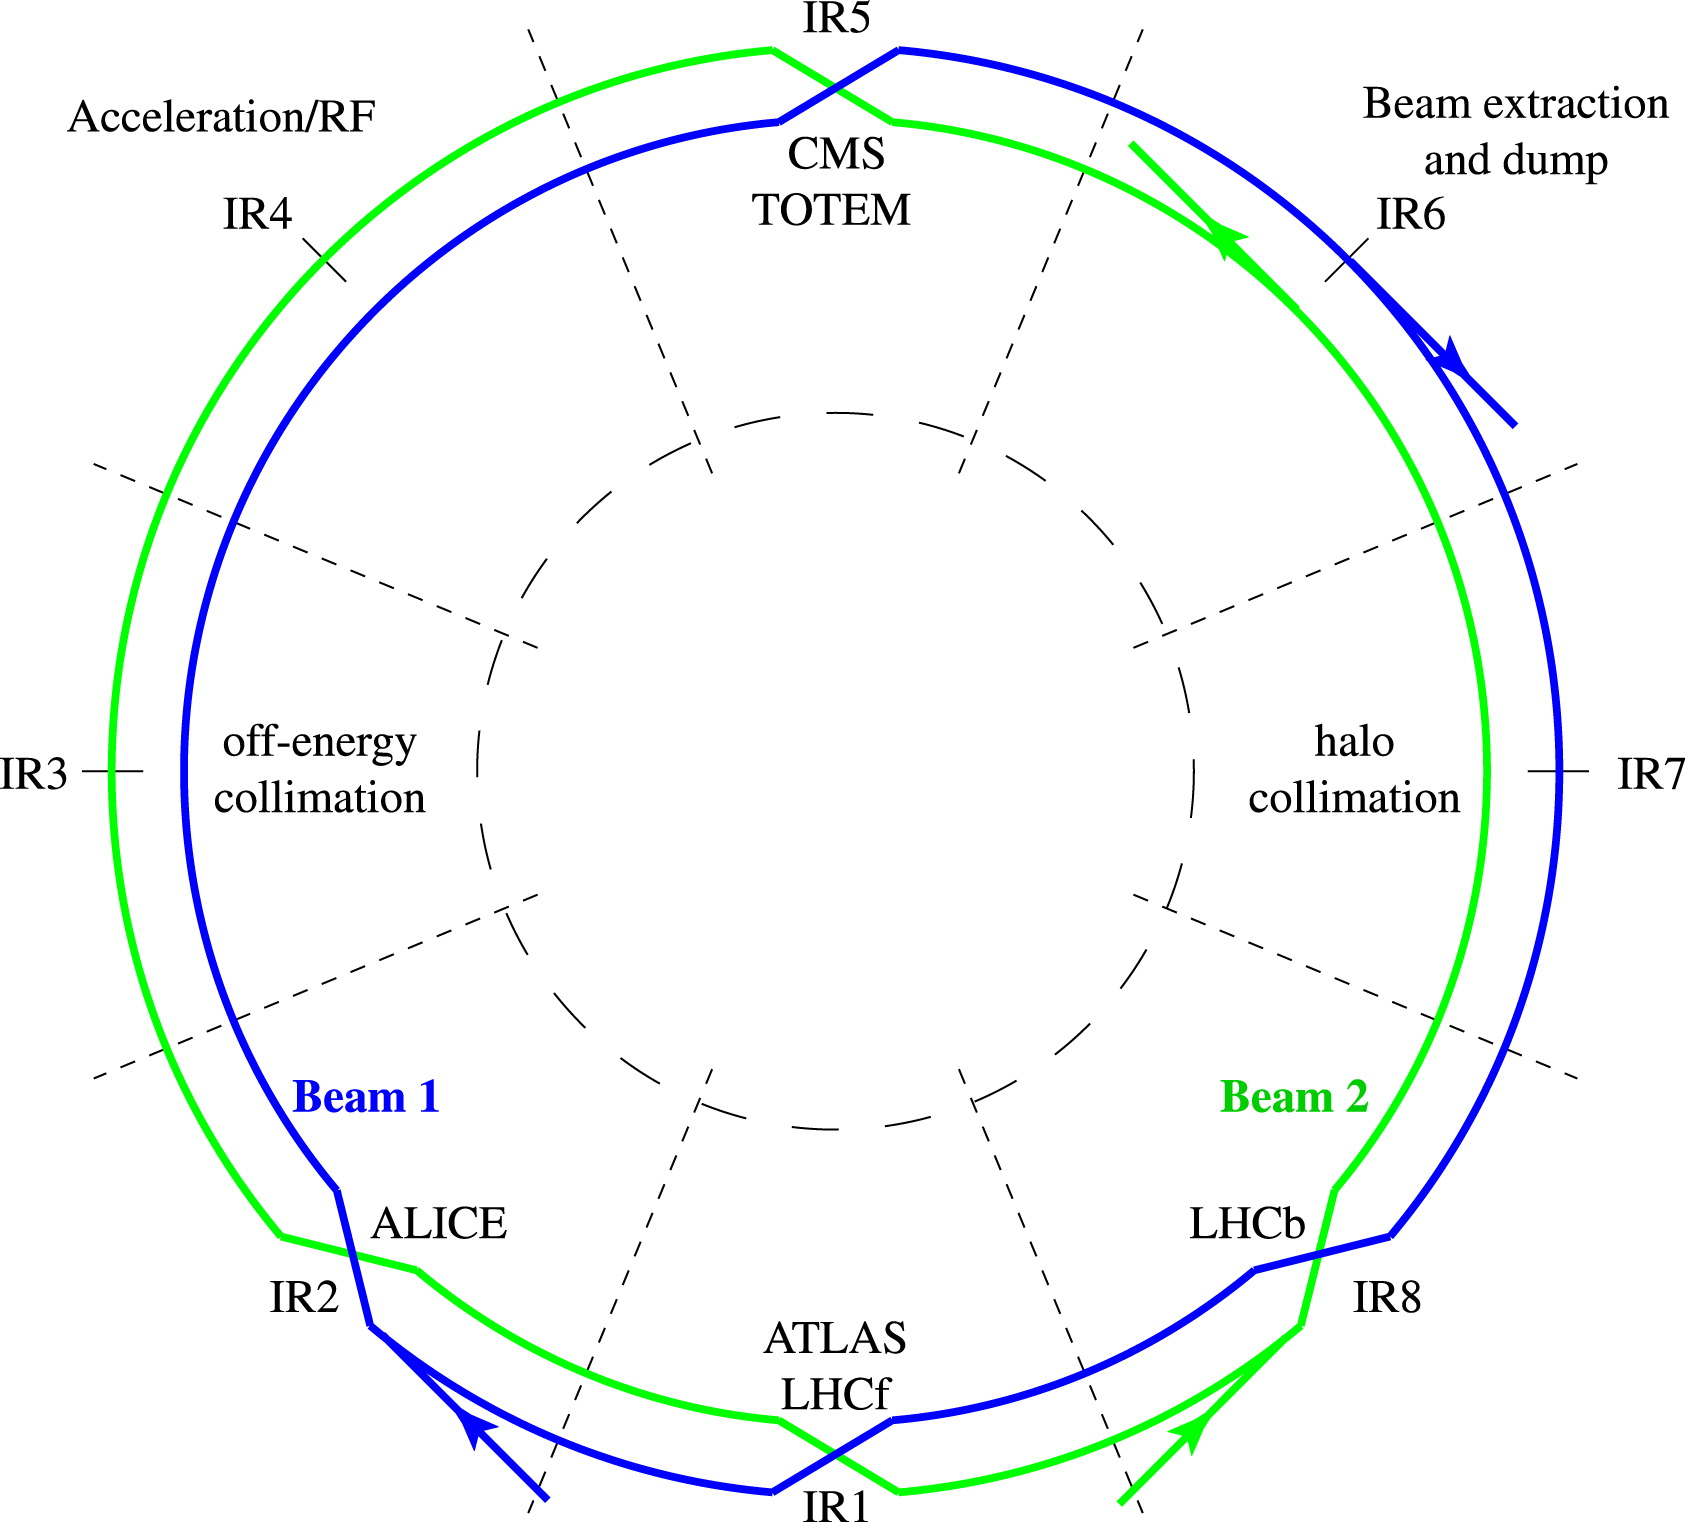
\includegraphics[width= 0.6\textwidth]{Figures/Chapter3/LHC_BasicLayout.jpg}
\caption[Basic schematic layout of the Large Hadron Collider]{Basic schematic layout of the LHC consisting of 8 arc sections along with the two circulating beams. The locations of the ATLAS, ALICE, CMS, and LHCb experiments are also displayed. Figure taken from Ref.~\cite{LHC_BasicLayout}.}
\label{Figure:Chapter3_LHC_BasicLayout}
\end{figure}

\newpage
Before entering the LHC ring, protons are ramped up through a series of pre-accelerator stages. The LHC represents the final link in this injector chain~\cite{LHC_InjectorComplex}, as shown in Fig.~\ref{Figure:Chapter3_LHC_Complex}. The first step is the \textbf{\ac{LINAC4}}~\cite{LINAC4}, where hydrogen gas is ionised to produce negative hydrogen ions and accelerated to $160\MeV$ for injection into the \textbf{\ac{PSB}}. During injection into the PSB, electrons are stripped off, leaving a pure proton beam that the PSB then accelerates to $2.0\GeV$. From there, the beam enters the \textbf{\ac{PS}}, raising its energy to $26\GeV$, before moving on to the \textbf{\ac{SPS}}, which boosts it to $450\GeV$. The beam is then injected into the LHC, where its energy is ramped up to several $\TeV$ in less than half an hour.

\begin{figure}[h]
\centering
\includegraphics[width= 0.85\textwidth]{Figures/Chapter3/LHC_AcceleratorComplex.pdf}
\caption[Schematic diagram of the CERN accelerator complex]{Schematic diagram of the CERN accelerator complex. Figure taken from Ref.~\cite{LHC_InjectorComplex}.}
\label{Figure:Chapter3_LHC_Complex}
\end{figure}

The \textbf{LHC} \textit{functions as a synchrotron accelerator}: protons continuously circulate the ring while radio-frequency (RF) cavities incrementally boost their energy. The strength of the bending magnets increases in synchrony with the rising beam momentum, allowing the particles to remain on a fixed trajectory. A network of 1,232 superconducting niobium-titanium dipole magnets, cooled to $1.9\unit{K}$ with superfluid helium, generates magnetic fields of up to $8.4\unit{T}$ to guide the beams along their circular path. At each of the four principal collision points, inner triplet quadrupole magnets compress the beams to reduce their transverse size, effectively squeezing them to maximise collision rates. These specifications reflect the accelerator complex's capabilities following upgrades completed during the most recent long shutdown.

\subsection{Cross section and Luminosity}

\textit{Cross section} and \textit{luminosity} are essential for predicting collision rates in the detector. The cross-section $\sigma(\sqrt{s})$ describes the probability of a given process occurring at centre-of-mass energy $\sqrt{s}$. However, knowing how often collisions occur also depends on how many particles are available to interact, which is described by the \textit{instantaneous luminosity} ($\mathscr{L}$). This quantity measures the number of particles passing through a unit area per unit time at the interaction point and depends on the detailed structure of the beams.

Since the proton beams at the LHC are not continuous streams but are composed of discrete bunches, the temporal structure of the beams directly impacts the collision frequency. Each bunch contains roughly $1.1\times10^{11}$ protons. During Run 2, the beams carried up to 2,220 bunches in 2016 and 2,556 bunches in 2017-2018. In 2022–2023, this number increased to a maximum of 2,808 bunches per beam, with bunches spaced by $25\unit{ns}$, corresponding to a crossing rate of $40\unit{MHz}$. The number of bunches, the number of protons per bunch, and the bunch spacing together determine the beam intensity and collision frequency, and therefore contribute directly to the luminosity. The dependence of the instantaneous luminosity on the beam parameters can be expressed as:

\begin{equation_pad}
\begin{aligned}
    \mathscr{L} &= \gamma \frac{n_b N^2 f_{\text{rev}}}{4\pi \beta^* \epsilon_n} R \\
    R &= 1 / \sqrt{1 + \left( \frac{\theta_c \sigma_z}{2\sigma} \right) }
\end{aligned}
\end{equation_pad}

where $\gamma$ is the proton beam energy expressed in rest mass units, $n_b$ is the number of bunches per beam, $N$ is the number of particles per bunch, $f_{rev}$ is the revolution frequency, $\beta^*$ is the beam beta function at the collision point and $\epsilon_n$ is the normalised transverse beam emittance. The term R is a geometrical reduction factor for luminosity. This is expressed as a function of the crossing angle of the beams at the collision point ($\theta_c$) and the transverse(longitudinal) spread of the particle bunch, $\sigma_z(\sigma)$. 

Because the beam parameters evolve over time, the luminosity is not constant. Therefore, the more appropriate quantity is the \textit{integrated luminosity} ($\mathscr{L}_{int}$), which represents the total data collected over a given period:

\begin{equation_pad}
    \mathscr{L}_{int} = \int \mathscr{L}(t) dt
\end{equation_pad}

The total number of events $(\mathscr{N})$ for a particular process with cross-section $\sigma$ over a fixed period can then be expressed as:

\begin{equation_pad}
    \mathscr{N} = \sigma \cdot \mathscr{L}_{int}
\end{equation_pad}

A summary of the total integrated luminosity delivered to the CMS experiment since 2015 is provided in Fig.~\ref{Figure:Chapter3_CMS_IntegratedLumi}.

\begin{figure}[h]
\centering
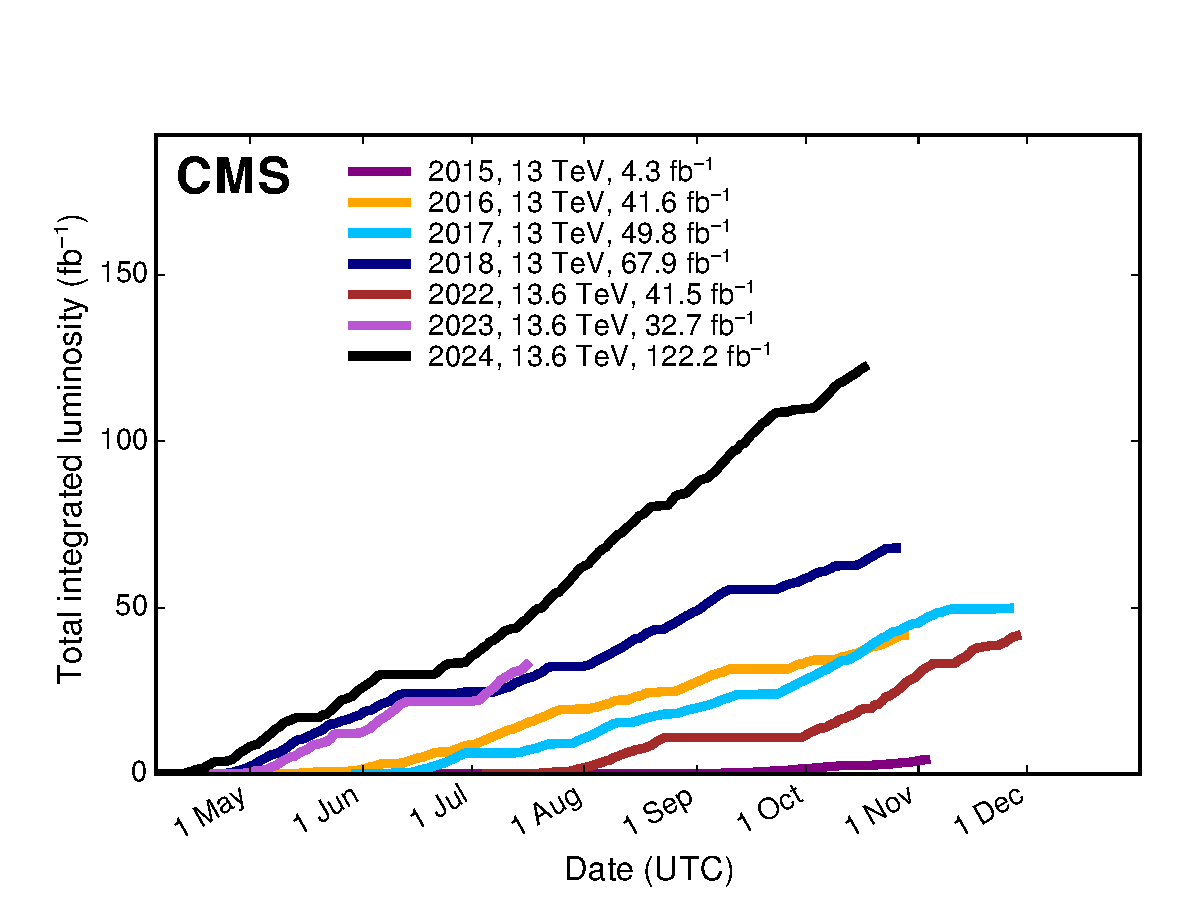
\includegraphics[width= 0.7\textwidth]{Figures/Chapter3/CMS_IntegratedLumi.pdf}
\caption[Total integrated luminosity delivered to the CMS experiment between 2015 and 2024]{Total integrated luminosity delivered to the CMS experiment between 2015 and 2024. Data collected from all periods except 2015 and 2024 are used in this thesis. Figure taken from Ref.~\cite{CMS_IntegratedLumi}.}
\label{Figure:Chapter3_CMS_IntegratedLumi}
\end{figure}

\subsection{Pileup}

To maximise the probability of observing rare processes, the LHC collides large bunches of protons, resulting in high instantaneous luminosity. However, this also introduces challenges: \textit{when bunches collide, multiple protons interact simultaneously, and the vast majority of these pp collisions do not involve a hard scattering process}. This means that for each event, the pp interaction of interest is recorded along with additional pp interactions, called \textbf{\ac{PU}} interactions. 

These PU interactions act as background noise, complicating the reconstruction of the primary hard-scattering event and degrading the performance of many physics measurements. As instantaneous luminosity increases, PU becomes more severe, and removing the unwanted overlap collisions requires increasingly sophisticated mitigation techniques. Figure~\ref{Figure:Chapter3_CMS_Pileup} displays the PU conditions encountered by the CMS experiment between 2015 and 2024.

\begin{figure}[h]
\centering
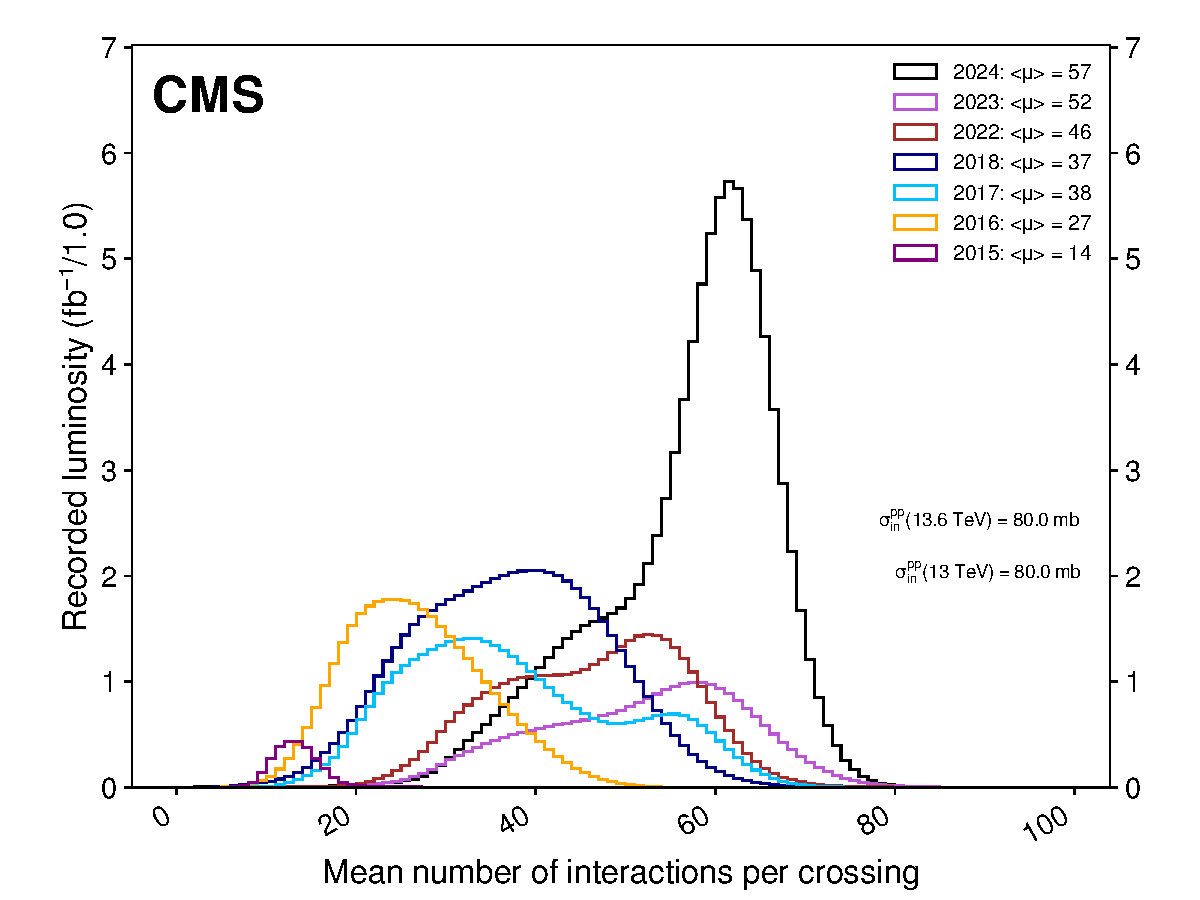
\includegraphics[width= 0.7\textwidth]{Figures/Chapter3/CMS_Pileup.pdf}
\caption[Distribution of the average number of interactions per bunch crossing for pp collisions at CMS between 2015 and 2024]{Distribution of the average number of interactions per bunch crossing for pp collisions between 2015 and 2024, using data from the CMS experiment. Figure taken from Ref.~\cite{CMS_IntegratedLumi}.}
\label{Figure:Chapter3_CMS_Pileup}
\end{figure}

\section{The CMS Detector}
\label{Section:Chapter3_CMS_Detector_Introduction}
CMS is one of the two general-purpose detectors at the LHC, built to explore a wide range of high-energy physics phenomena. The design of the CMS detector was shaped by the ambitious goals of the LHC physics programme~\cite{LHC_CMS}, which demanded precise and efficient measurements under challenging experimental conditions. To accomplish these objectives, several key performance requirements were identified:

\begin{itemize}
  \item Identification \& precise momentum reconstruction of muons over a broad range of momenta and angles; dimuon mass resolution $\sim1\%$ at $100\GeV$; unambiguous muon charge identification up to $1\TeV$
  \item High momentum resolution \& reconstruction efficiency for charged particles; efficient $\tau$‐lepton and b‐jet identification
  \item Photon/electron energy measurement with excellent resolution; diphoton and dimuon mass resolution $\sim1\%$ at $100\GeV$ over a wide geometrical coverage
  \item Effective $\pi^0$ rejection; efficient isolation of photons and leptons in high‐luminosity, high‐occupancy conditions
  \item Precise dijet mass reconstruction and MET resolution
\end{itemize}

CMS employs a compact, layered detector system arranged cylindrically around the interaction point to fulfil these performance requirements, providing nearly 4$\pi$ solid-angle coverage. The entire detector is $21.6\unit{m}$ long and has a diameter of $14.6\unit{m}$ while weighing $12,500\unit{t}$. This makes CMS one of the largest yet compact detectors ever engineered for a particle physics experiment. Closest to the beam pipe lies the \textbf{silicon tracker}, which precisely tracks charged particles. It is surrounded by the \textbf{\ac{ECAL}}, optimised for measuring the energy of electrons and photons with high precision. The \textbf{\ac{HCAL}} follows and is responsible for absorbing and measuring the energy of hadrons. These three subdetectors are enclosed within a powerful $13\unit{m}$ long, $6\unit{m}$ inner-diameter, $3.8\unit{T}$ \textbf{superconducting solenoid}. Embedded within the iron return yoke of the solenoid is the \textbf{muon detection system}. A schematic of the full CMS detector is shown in Fig.~\ref{Figure:Chapter3_CMS_schematic}, providing an overview of its cylindrical geometry and layered structure around the LHC interaction point. The following sections will provide a more detailed discussion of each of the major subdetector systems introduced here. A complementary longitudinal slice through the detector is shown in Fig.~\ref{Figure:Chapter3_CMS_slice}, serving as a visual reference for the detailed subdetector descriptions that follow.

\begin{figure}[h]
\centering
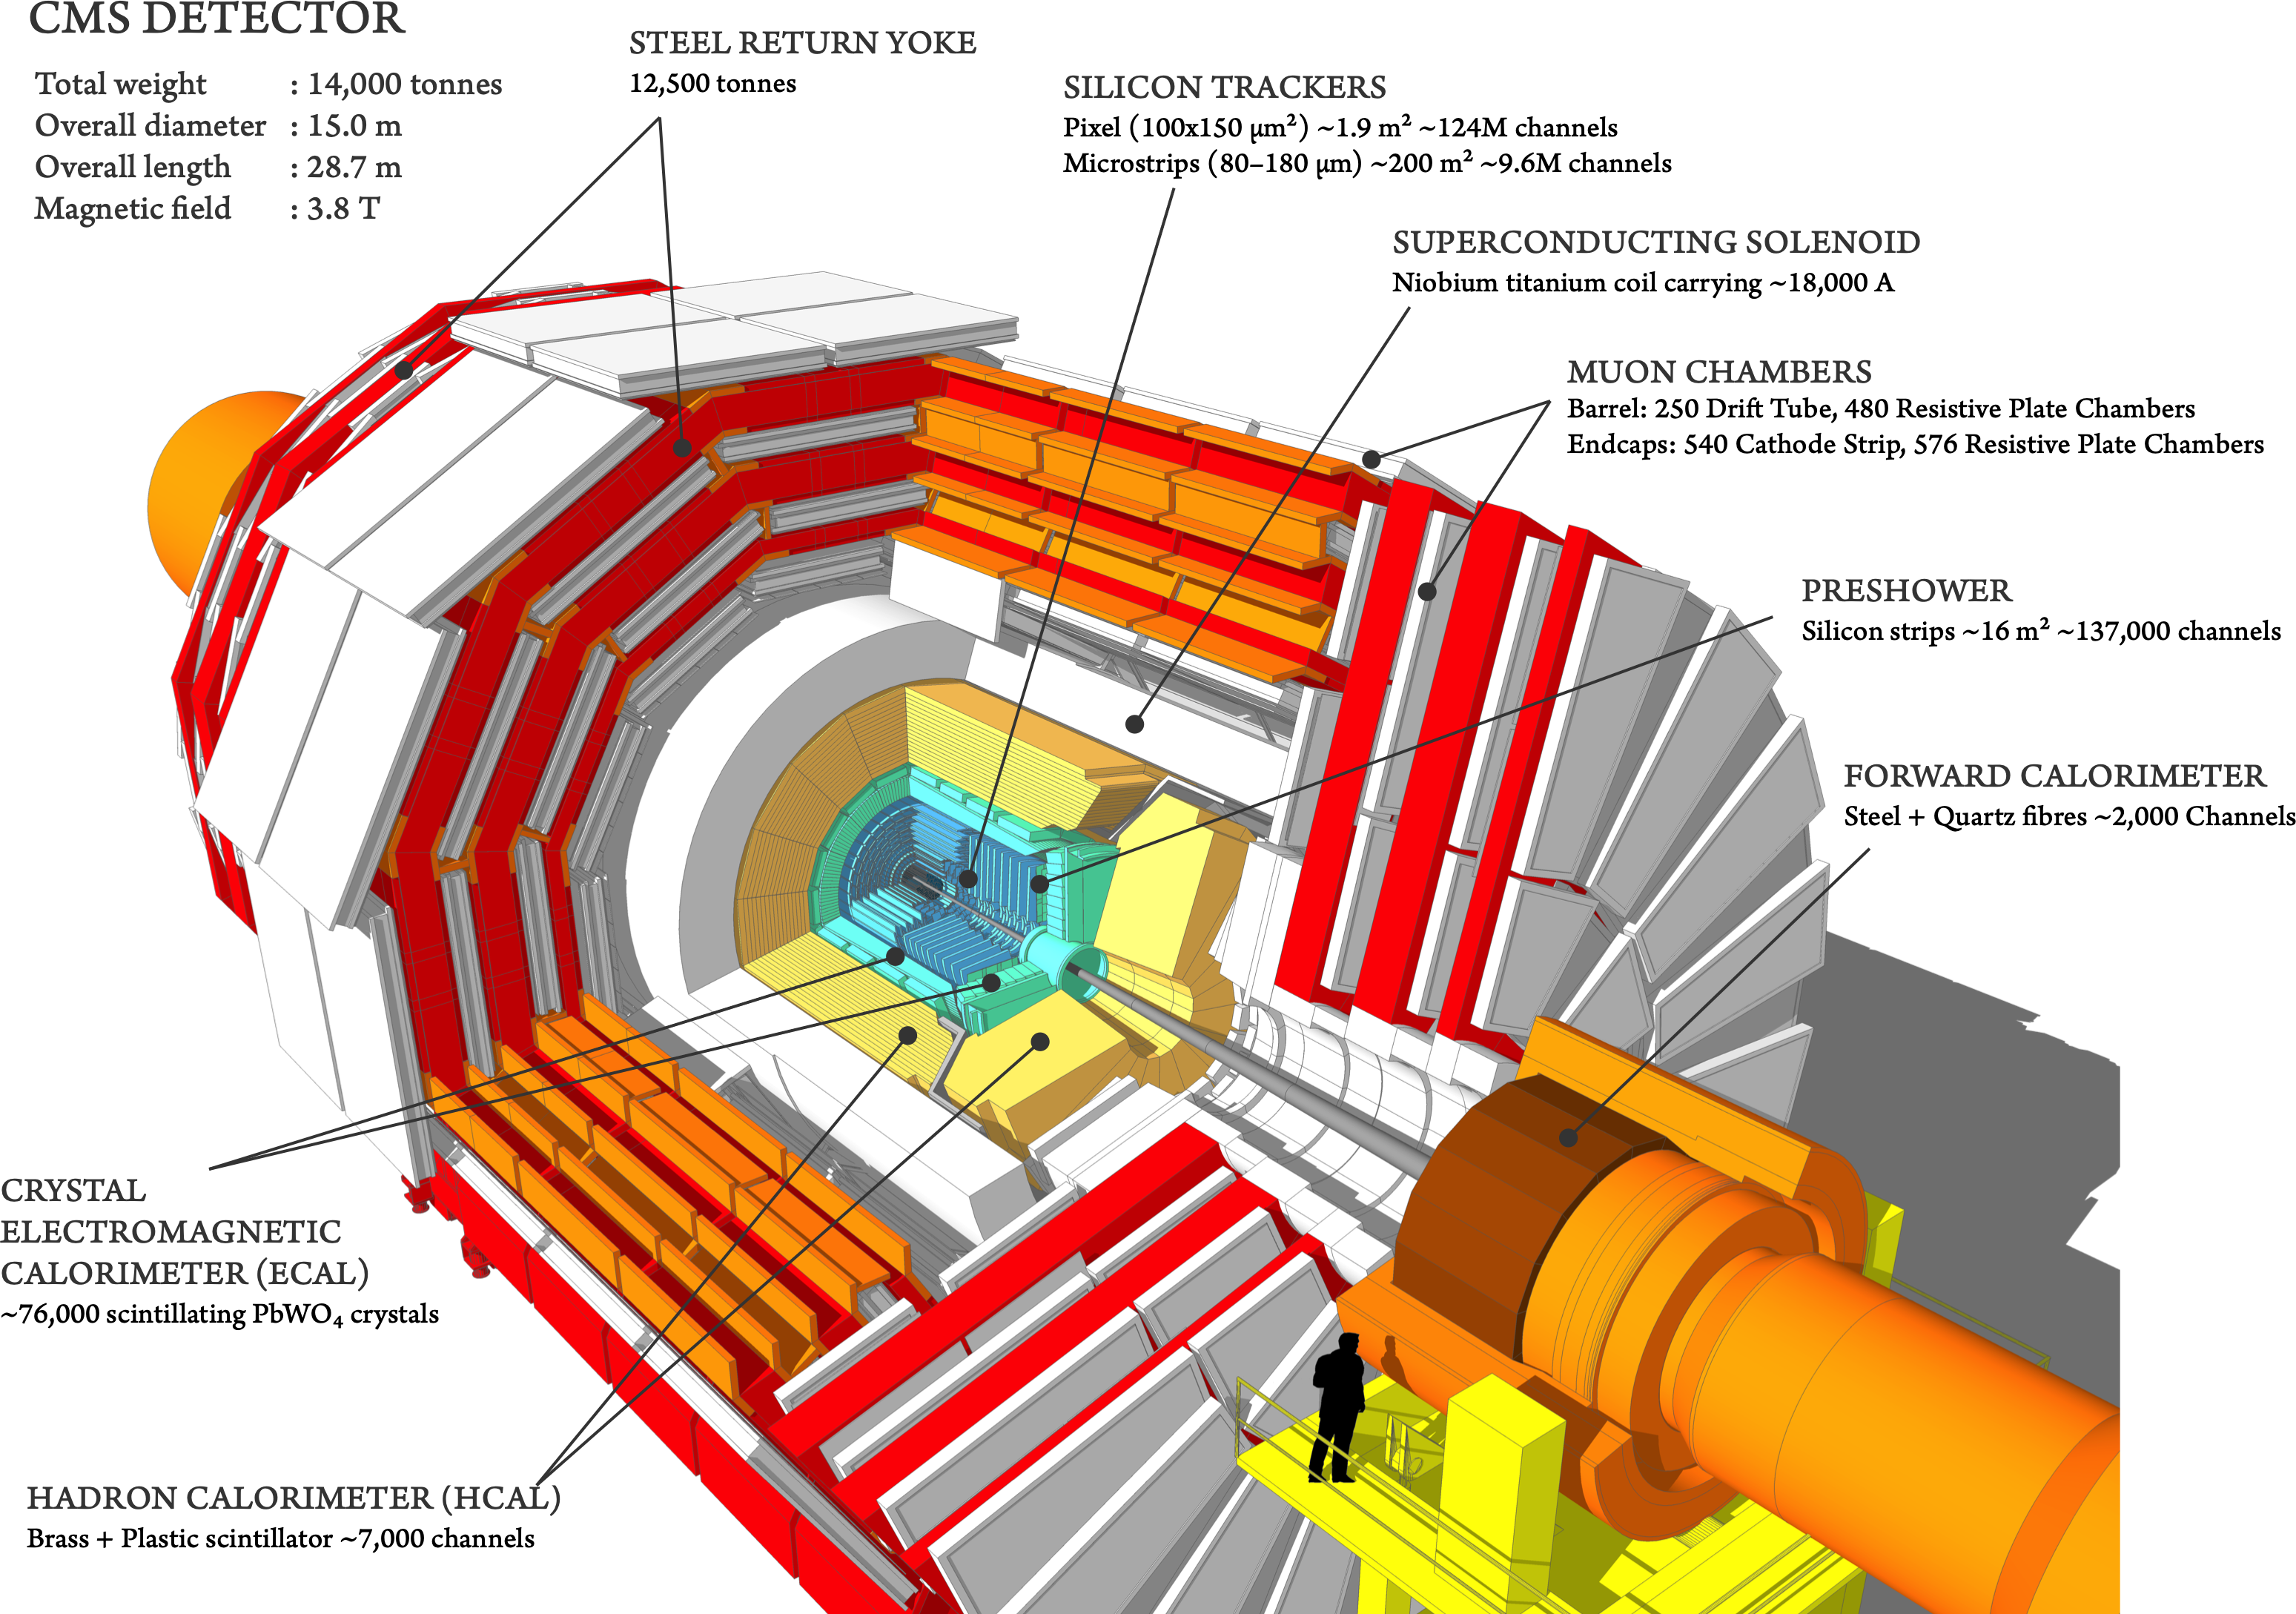
\includegraphics[width= 0.8\textwidth]{Figures/Chapter3/CMS_Detector.pdf}
\caption[Schematic drawing of the CMS detector]{Schematic drawing of the CMS detector. Figure taken from Ref.~\cite{CMS_Detector_Run3}.}
\label{Figure:Chapter3_CMS_schematic}
\end{figure}

\begin{figure}[h]
\centering
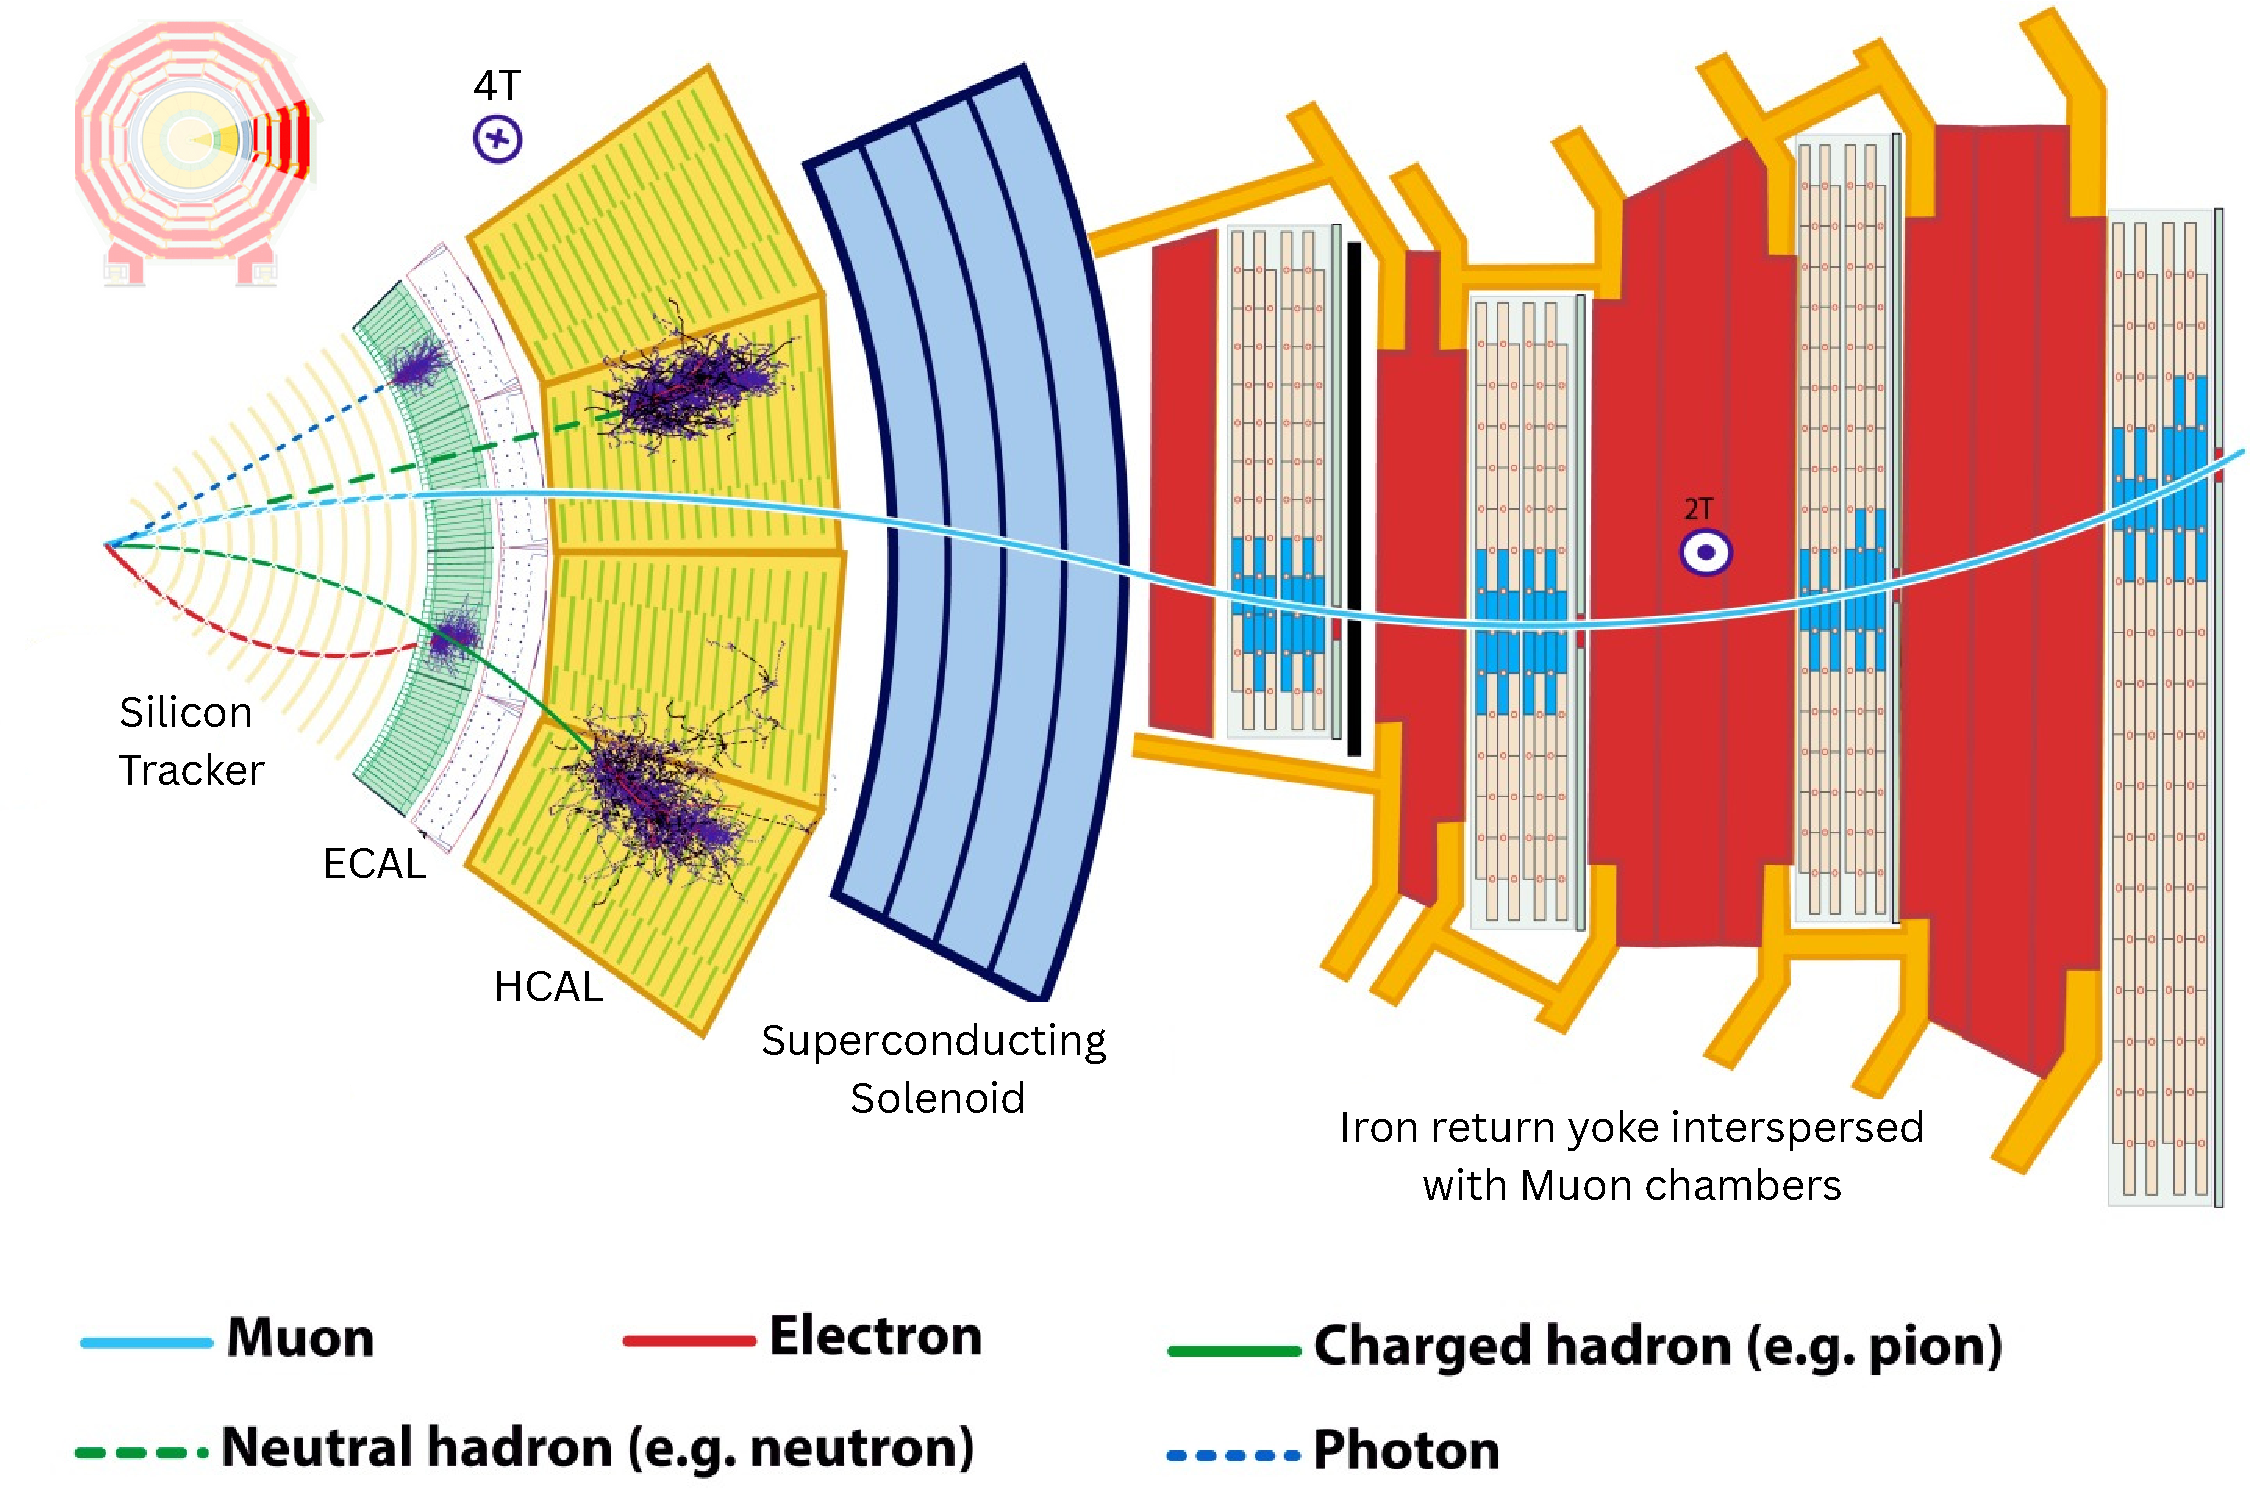
\includegraphics[width= 0.8\textwidth]{Figures/Chapter3/CMS_Detector_Slice.pdf}
\caption[Transverse slice of the CMS detector]{A transverse slice of the CMS detector displaying the individual subsystems and their response to different types of particles. Figure adjusted from Ref.~\cite{CMS_Detector_Slice}.}
\label{Figure:Chapter3_CMS_slice}
\end{figure}

\clearpage
\subsection{Co-ordinate system}
CMS adopts a right-handed Cartesian coordinate system centred at the nominal collision point. The $x$-axis points towards the centre of the LHC ring, and the $y$-axis points vertically upwards, while the $z$-axis points along the beam direction towards the Jura mountains, as illustrated in Fig.~\ref{Figure:Chapter3_CMS_CoordinateSystem}.

\begin{figure}[h]
\centering
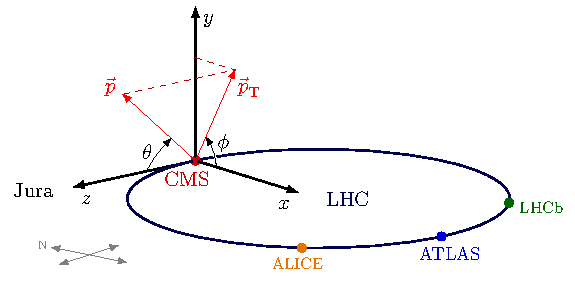
\includegraphics[width= 0.8\textwidth]{Figures/Chapter3/CMS_CoordinateSystem.pdf}
\caption{The CMS detector coordinate system.}
\label{Figure:Chapter3_CMS_CoordinateSystem}
\end{figure}

In this system, the plane perpendicular to the beam axis, $x-y$ plane, is referred to as the \textit{transverse plane}, while the $z$-axis defines the \textit{longitudinal direction}. The \textit{azimuthal angle} $\phi \in [0,2\pi]$ is the angle with respect to the positive $x$-axis in the transverse plane, while the \textit{polar angle} $\theta \in [0,\pi]$ is with respect to the $z$-axis. Rather than using $\theta$ directly, it is common in collider physics to introduce \textit{pseudorapidity} ($\eta$), defined as

\begin{equation_pad}
    \eta = - \ln\left[\tan(\theta/2)\right]
\end{equation_pad}

A key property of this quantity is that the difference in pseudorapidity ($\Delta\eta$) between two vectors is invariant under Lorentz boosts along the longitudinal $z$-axis. This is convenient in hadron collider experiments, where the parton-parton centre-of-mass frame is often significantly boosted along the beam direction due to the variable momentum fractions carried by the incoming partons. Additionally, $\eta$ provides a nearly linear mapping of $\theta$ (shown in Fig.~\ref{Figure:Chapter3_Pseudorapidity}), facilitating a simple description of particle emission angles relative to the beam axis. This property allows for a natural segmentation of the detector into barrel and endcap regions based on $\eta$.

\begin{itemize} 
\item \textbf{Barrel region}: The central cylindrical region of the detector, located closest to the primary interaction point and optimised for particles emitted at large angles to the beamline ($\ie$ low $|\eta|$). 
\item \textbf{Endcap regions}: Located at either end of the barrel along the $z$-axis, designed to detect particles emitted at small angles with respect to the beamline ($\ie$ high $|\eta|$). 
\end{itemize}

\begin{figure}[h]
\centering
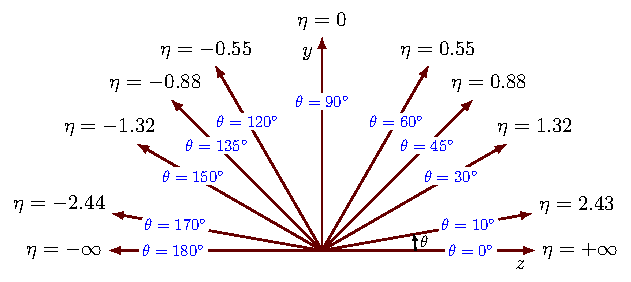
\includegraphics[width= 0.8\textwidth]{Figures/Chapter3/Pseudorapidity.pdf}
\caption{Illustration of the relationship between pseudorapidity ($\eta$) and polar angle ($\theta$).}
\label{Figure:Chapter3_Pseudorapidity}
\end{figure}

At the LHC, the initial momentum component of the system perpendicular to the beam axis is nearly zero because of the head-on nature of the beam. This kinematic quantity is referred to as the transverse momentum ($p_\mathrm{T}$) and is defined as:

\begin{equation_pad}
    p_\mathrm{T} = \sqrt{p_x^2 + p_y^2}
\end{equation_pad}

Transverse momentum is a central observable in collider physics. It provides a direct probe of hard interaction processes characterised by large momentum transfers. A complementary quantity to the transverse momentum is the missing transverse momentum ($E_\mathrm{T}^{\text{miss}}$), which is defined as the negative vector sum of the transverse momenta of all reconstructed particles in an event. This is a critical quantity serving as an estimator of the transverse momentum carried by non-interacting or undetected particles.

The radial distance from the beam axis is typically expressed as $r = \sqrt{x^2+y^2}$. Additionally, it is also convenient to express the distance metric ($\Delta R$) between two objects in a Lorentz-invariant way as:

\begin{equation_pad}
    \Delta R = \sqrt{(\Delta\eta)^2 + (\Delta \phi)^2}
\end{equation_pad}

This quantity is important in object reconstruction, as discussed in Section~\ref{Section:Chapter4}.%

\subsection{Magnet System}

As its name implies, CMS is defined by its central feature: the solenoid magnet. This critical component generates a very strong magnetic field that bends the trajectories of charged particles as they traverse the detector. This enables precise measurements of their momenta and electric charges. 

The \textbf{solenoid} spans $13\unit{m}$ in length and $6\unit{m}$ in diameter, capable of producing a magnetic field of up to $4\unit{T}$, but is currently operated at $3.8\unit{T}$ for enhanced long-term stability. The strong field ensures that low-momentum charged particles are sufficiently curved, confining them within the inner tracking system and aiding in precise momentum resolution. This not only improves tracking quality but also helps mitigate calorimeter noise by preventing soft particles from reaching the calorimeters.

Outside the solenoid, the muon detection system is embedded within segmented layers of iron, forming the \textbf{iron yoke}. This massive structure, weighing approximately $10,000\unit{t}$, serves two primary purposes: it returns about two-thirds of the magnetic flux generated inside the detector and provides structural support for the muon chambers. By returning the flux, the iron yoke significantly reduces the magnetic field outside the detector. This magnetic field configuration causes a ``\textit{double bending}'' of muon trajectories: first in one direction as muons pass through the inner silicon tracker, and then in the opposite direction as they traverse the muon chambers embedded in the iron yoke. This double bending significantly enhances the overall muon momentum resolution.

\subsection{Inner tracking system}
The CMS interaction point is surrounded by the innermost subdetector, the \textbf{silicon tracker}, which measures $5.8\unit{m}$ in length and $2.5\unit{m}$ in diameter~\cite{LHC_CMS,CMS_Detector_Run3}. The tracker plays a central role in reconstructing the trajectories of charged particles and in identifying both primary and secondary interaction vertices with high spatial precision.

At the LHC’s design luminosity, on the order of $10^3$ charged particles traverse the tracker volume per each $25\unit{ns}$ bunch crossing. To cope with the extreme occupancy, the tracker must combine high granularity with rapid signal readout. Furthermore, its proximity to the interaction point exposes it to a harsh radiation environment, necessitating the use of radiation-hard sensor technologies to preserve long-term performance.

To meet these demanding requirements, the CMS tracker employs \textit{silicon-based sensors}. However, these silicon sensors also require dedicated readout electronics and active cooling systems. These components contribute to the non-active material within the tracking volume, which must be carefully controlled. Excessive material leads to increased multiple scattering and energy loss, degrading momentum resolution and negatively impacting the performance of outer subdetectors such as the calorimeters.

As shown in Fig.~\ref{Figure:Chapter3_Tracker_MaterialBudget}, the material budget of the tracker is kept as low as possible, particularly in the central (low-$\eta$) region of the pixel detector, where precision tracking is most critical.

\begin{figure}[h]
    \centering
    % First row
    \begin{subfigure}[b]{0.49\textwidth}
        \centering
        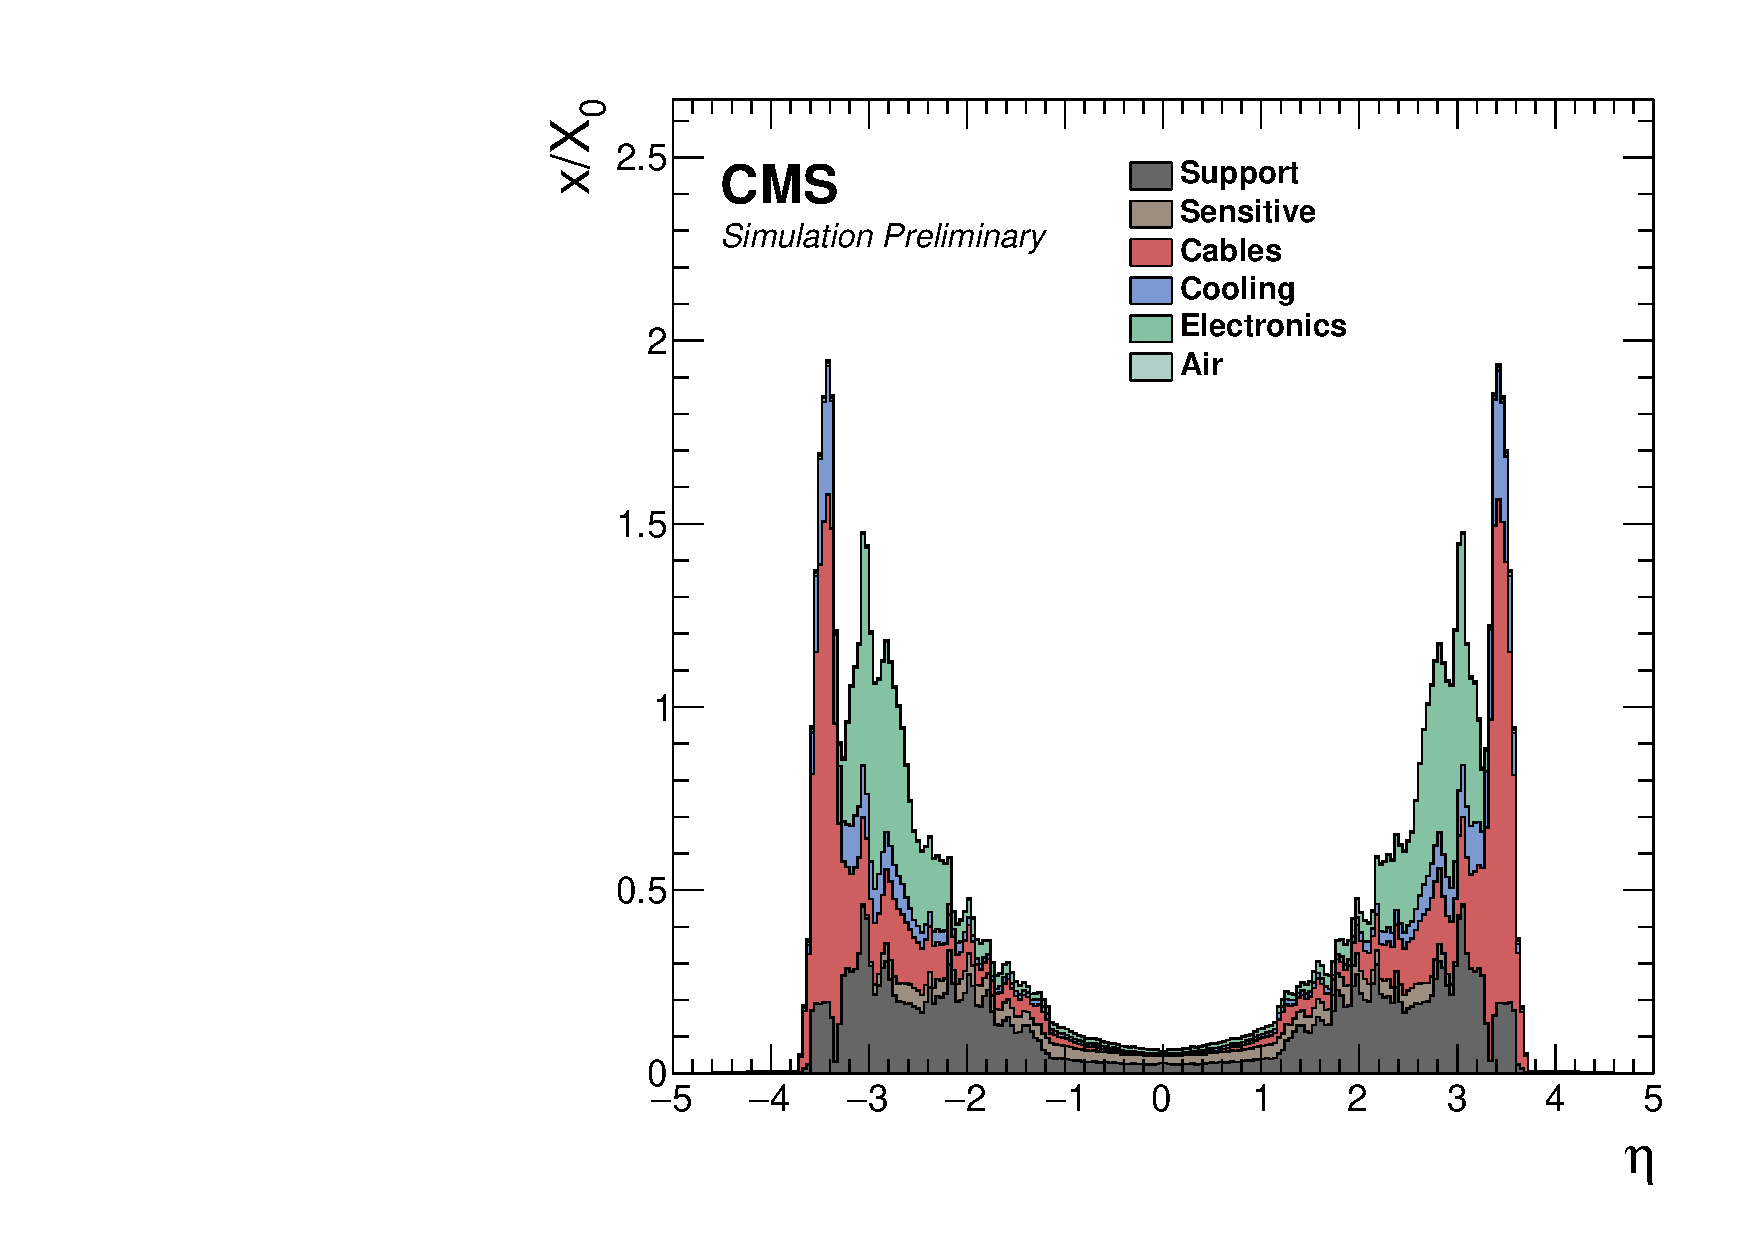
\includegraphics[width=\textwidth]{Figures/Chapter3/Material_Budget1.pdf}
        \caption{}
    \end{subfigure}
    \begin{subfigure}[b]{0.49\textwidth}
        \centering
        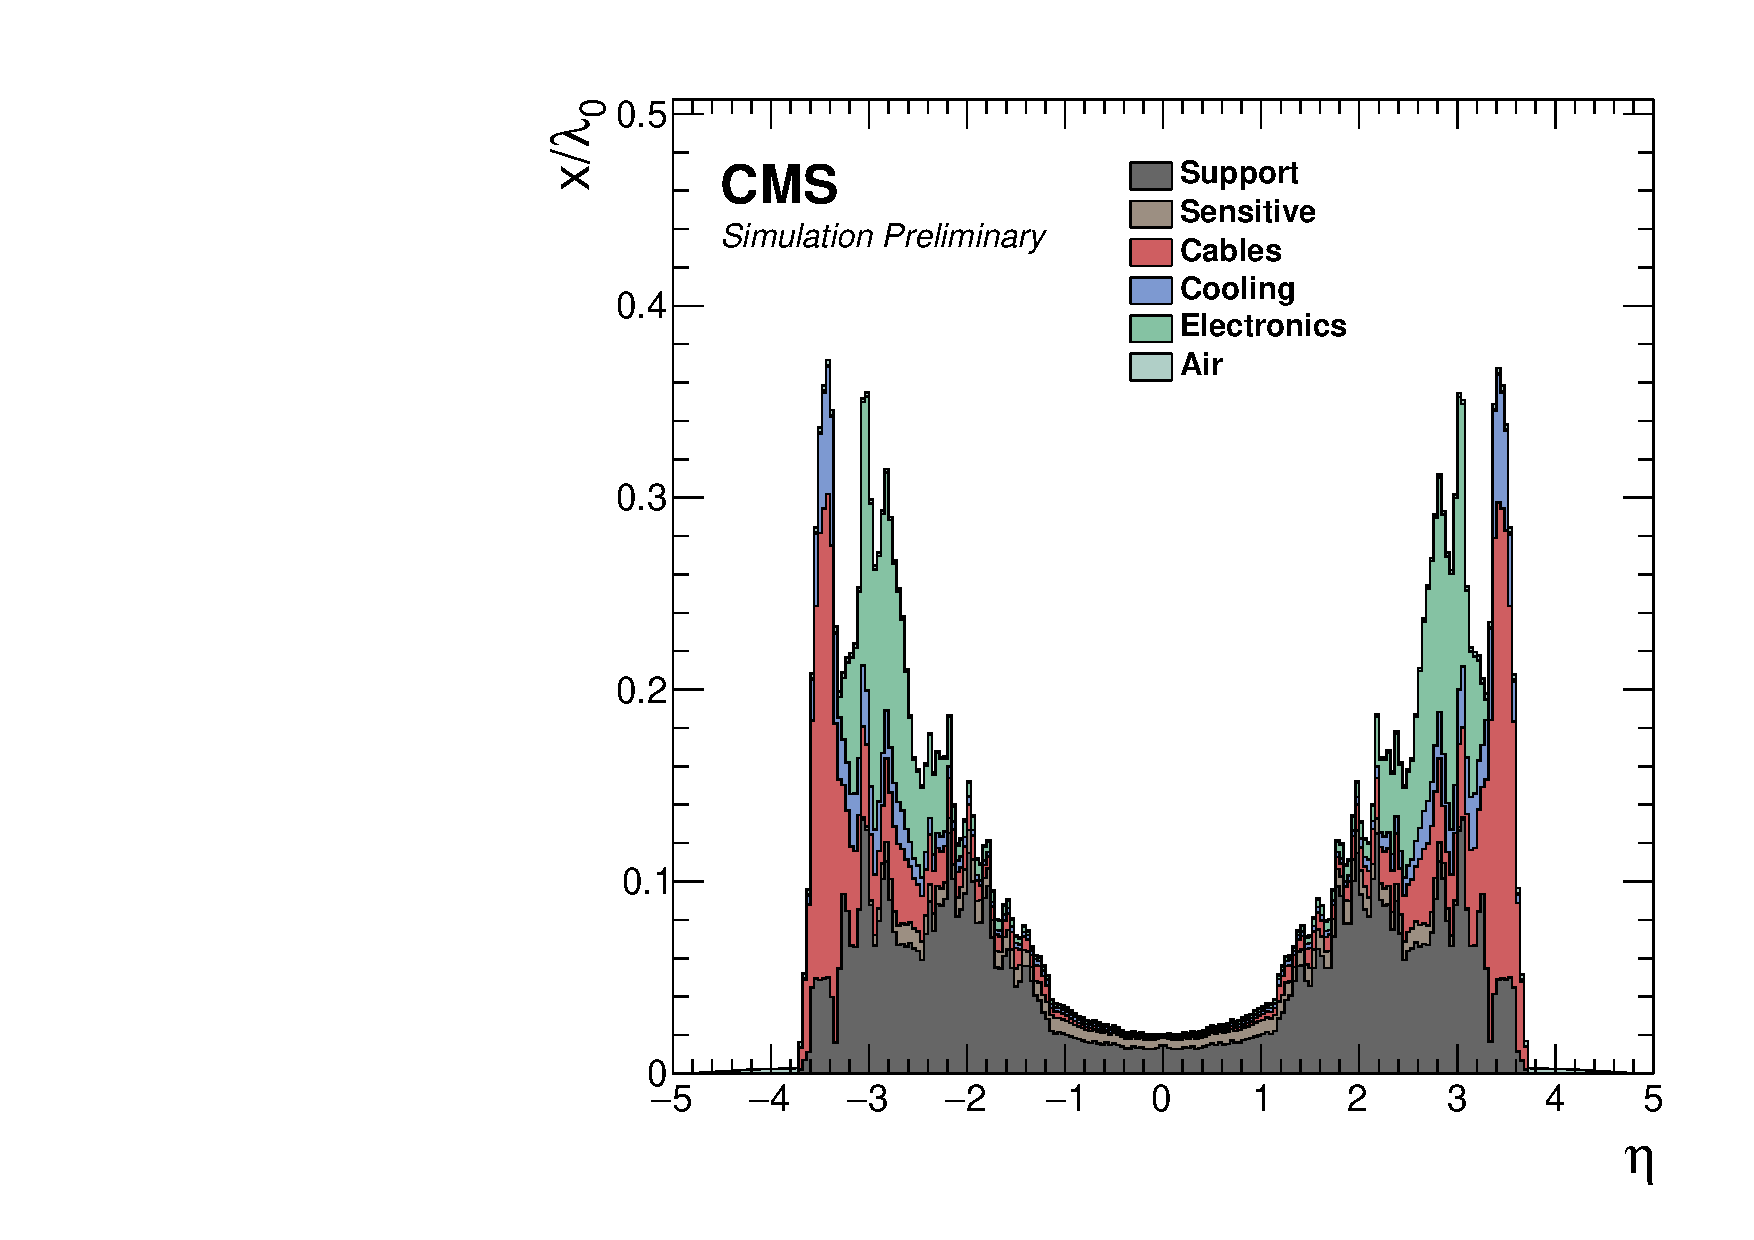
\includegraphics[width=\textwidth]{Figures/Chapter3/Material_Budget2.pdf}
        \caption{}
    \end{subfigure}
\caption[Simulation of the CMS pixel detector material budget]{Simulation of the CMS pixel detector material budget as a function of $\eta$ in units of ($\textbf{a}$) radiation length and ($\textbf{b}$) hadronic interaction length for different detector components. Figure taken from Ref.~\cite{TrackerMaterialBudget_Pixel}.}
\label{Figure:Chapter3_Tracker_MaterialBudget}
\end{figure}

\newpage
\subsubsection{Pixel Detector}

The innermost component of the CMS tracking system is the \textbf{silicon pixel detector}. The original pixel detector~\cite{LHC_CMS}, installed in 2008, was designed to operate for up to ten years under the LHC’s nominal instantaneous luminosity of $1 \times 10^{34}\unit{cm}^{-2}\unit{s}^{-1}$, with the capacity to handle up to 25 PU interactions ber bunch crossing. However, even during Run-1, the LHC exceeded its design luminosity, exposing the pixel detector to increased radiation levels and causing rising readout inefficiencies. To maintain high tracking efficiency under upgraded luminosity conditions of up to $2 \times 10^{34}~\unit{cm}^{-2}\unit{s}^{-1}$ and PU levels of 50 or more, the CMS pixel detector underwent a major upgrade in 2017, referred to as the Phase-1 upgrade~\cite{CMS_Detector_Run3, CMS_Tracker_Phase1_Upgrade}. This upgrade introduced a more granular and radiation-tolerant detector layout, featuring four barrel layers and three endcap disks.

The \textbf{\ac{BPIX}} detector consists of four concentric cylindrical layers (L1-L4) positioned at radii of 29, 68, 109, and 160$\unit{mm}$ from the beamline. A total of 1,184 sensor modules are deployed in the barrel region. Each module contains a silicon sensor segmented into $160 \times 416$ individual pixels with a pitch of $100 \times 150\unit{\mu m}^2$, enabling high-resolution hit detection. Compared to the original pixel detector, the innermost layer (L1) was also moved closer to the interaction point by reducing the CMS beam pipe radius from 30 to 23$\unit{mm}$ in 2014. 

The \textbf{\ac{FPIX}} detector complements the barrel coverage by extending tracking capabilities in the forward region. It comprises three endcap disks on each side of the detector, located at distances of 291, 396, and 516$\unit{mm}$ from the interaction point. The forward region is equipped with 672 pixel modules, featuring the same fine segmentation and pixel pitch as the barrel modules. Together, the BPIX and FPIX systems provide approximately 124 million readout channels, ensuring precise tracking throughout the detector’s angular coverage.

The Phase-1 upgrade of the CMS pixel detector introduced significant improvements in geometry and coverage, as illustrated in Fig.~\ref{Figure:Chapter3_Pixel_Upgrade}. Additionally, substantial gains were also achieved in spatial resolution and tracking performance. The position resolution reaches approximately $11\unit{\mu m}$ in the $r-\phi$ direction and $24\unit{\mu m}$ in the $z$ direction for BPIX L3. Somewhat worse resolutions are observed in the innermost barrel layers due to higher radiation damage. For FPIX, the corresponding resolutions are about $12\unit{\mu m}$ ($r$) and $21\unit{\mu m}$ ($z$). 

\begin{figure}[h]
\centering
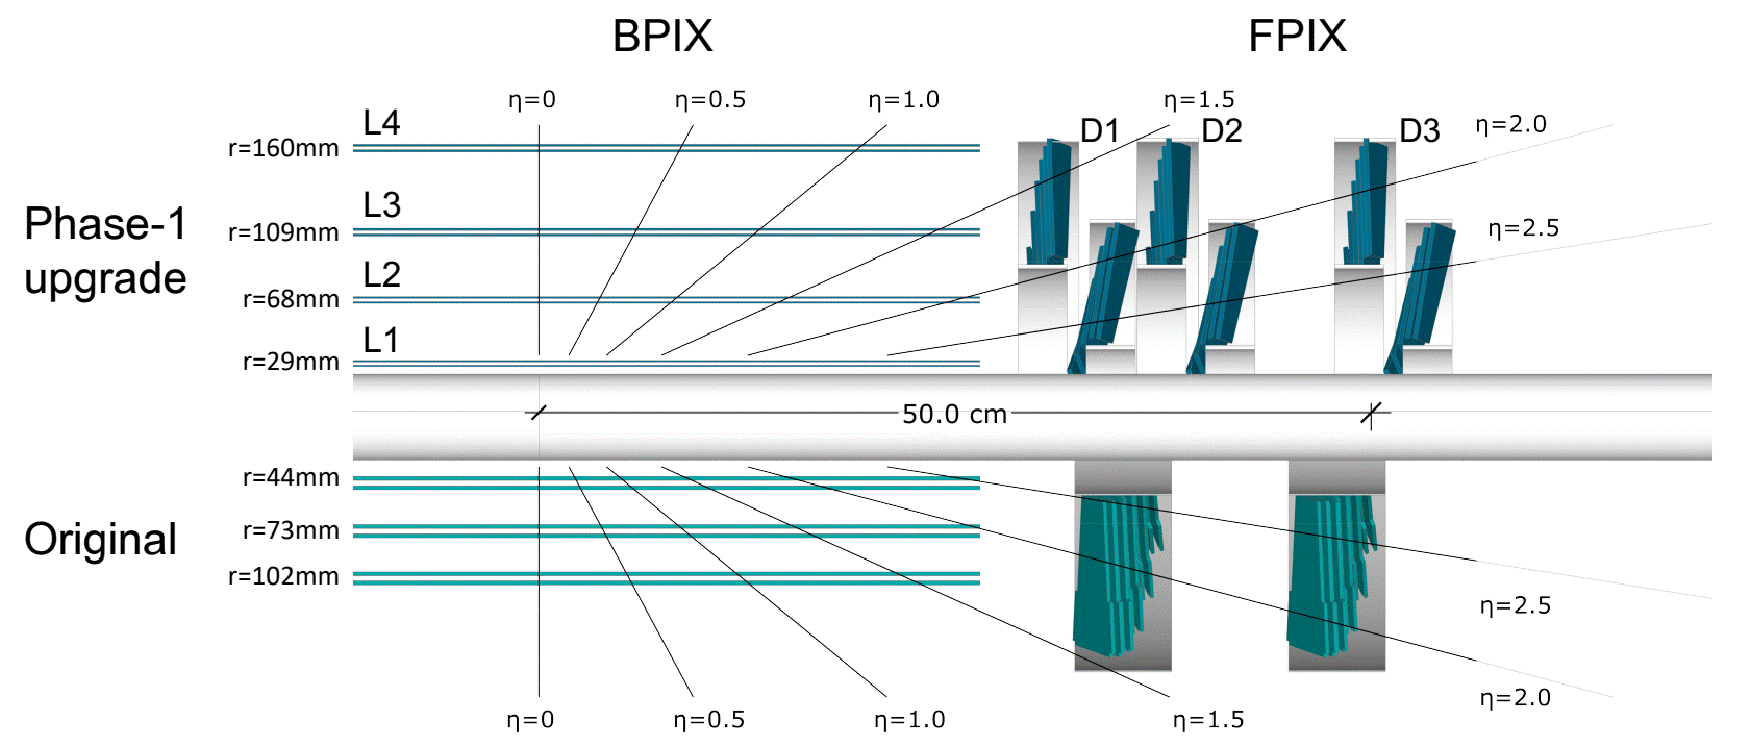
\includegraphics[width=1\textwidth]{Figures/Chapter3/CMS_Pixel_Upgrade.pdf}
\caption[Longitudinal view of CMS pixel detector before and after Phase-1 Upgrade]{Longitudinal view of CMS pixel detector comparing its structure before (lower part) and after (upper part) the Phase-1 Upgrade. Figure taken from Ref.~\cite{CMS_Detector_Run3}.}
\label{Figure:Chapter3_Pixel_Upgrade}
\end{figure}

The improved granularity and four-hit coverage introduced in the Phase-1 pixel detector enable robust three-dimensional reconstruction of charged particle trajectories, which is essential for precise identification of both primary and secondary vertices. Consequently, these tracking enhancements lead to improved vertex reconstruction performance. As shown in Fig.~\ref{Figure:Chapter3_Pixel_Vertex_Resolution}, the transverse ($x,y$) vertex resolution achieved with the Phase-1 detector is significantly better than that of the Phase-0 detector.

\begin{figure}[h]
    \centering
    % First row
    \begin{subfigure}[b]{0.49\textwidth}
        \centering
        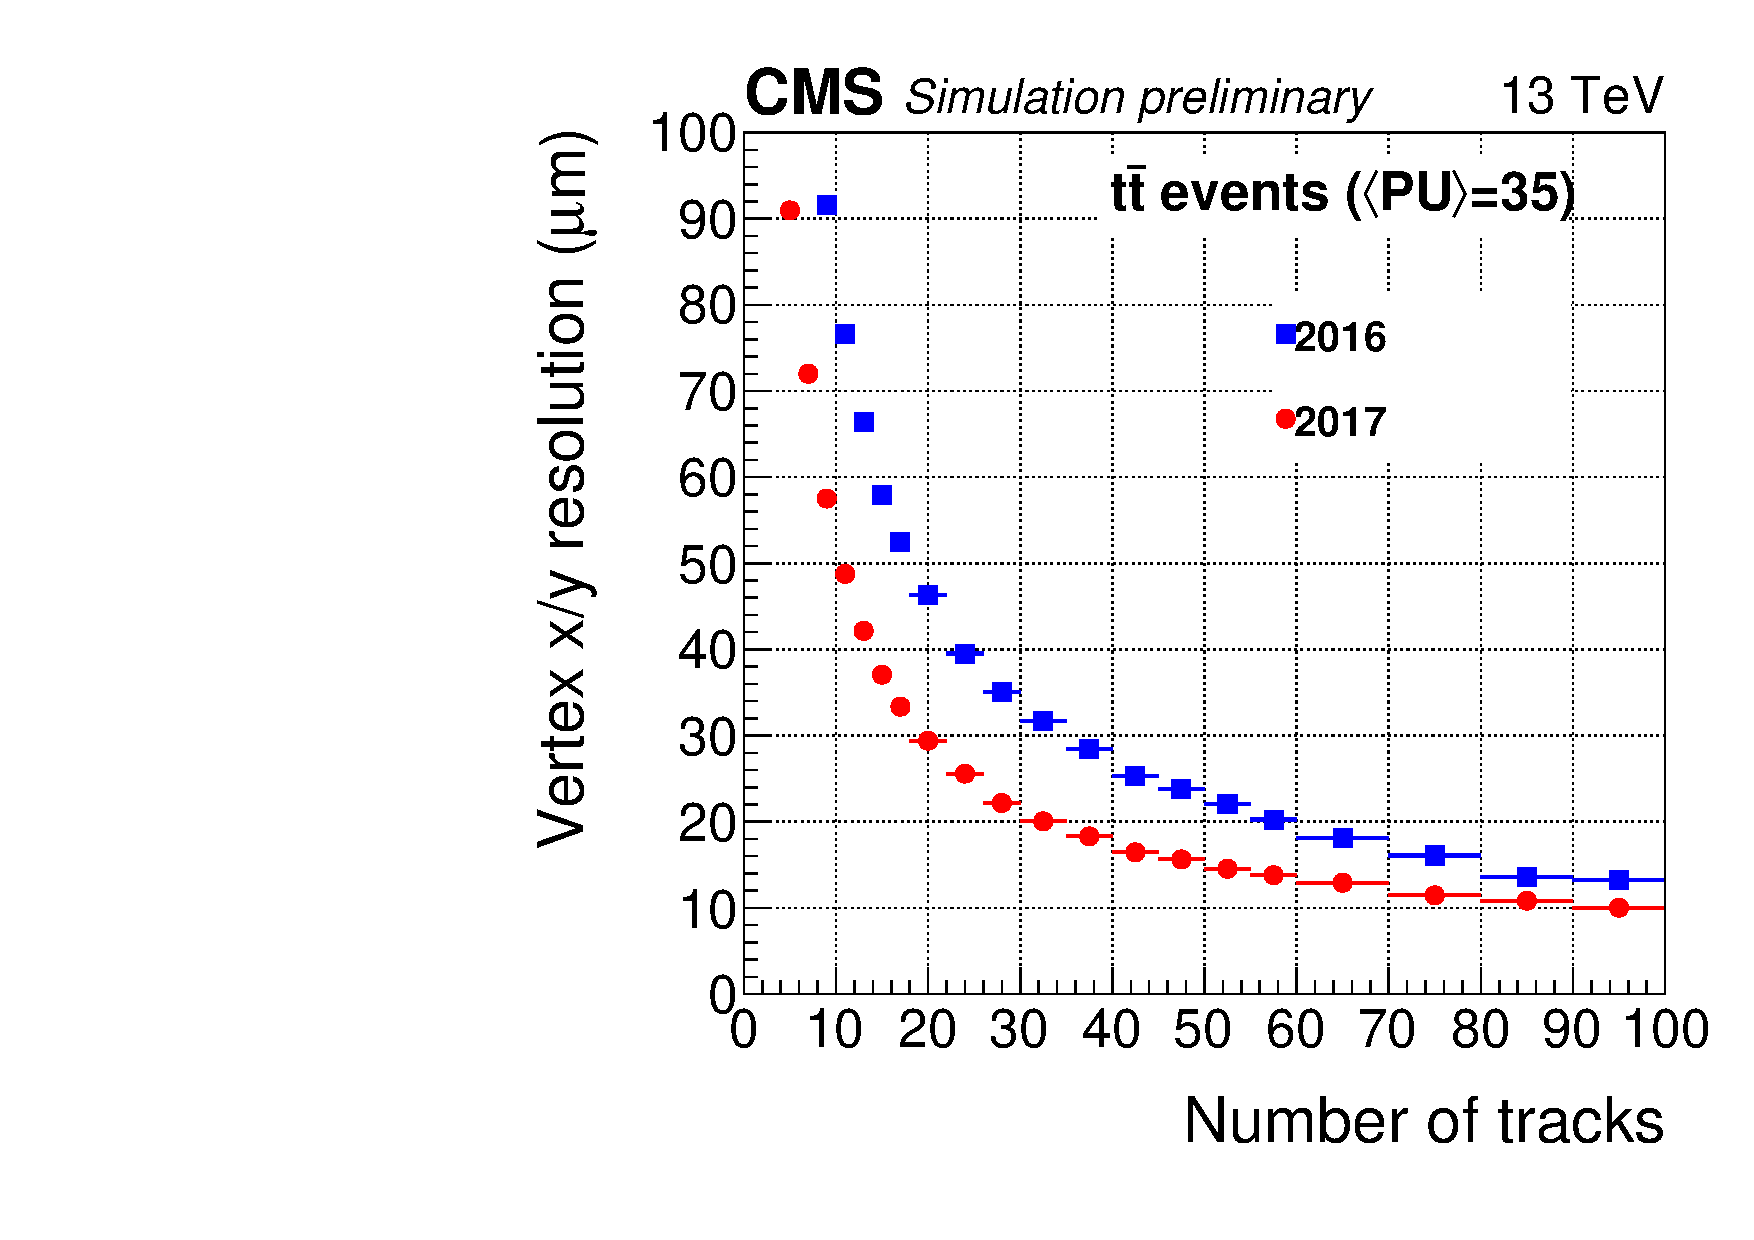
\includegraphics[width=\textwidth]{Figures/Chapter3/Pixel_Vertex_XY_Resolution.pdf}
        \caption{}
    \end{subfigure}
    \begin{subfigure}[b]{0.49\textwidth}
        \centering
        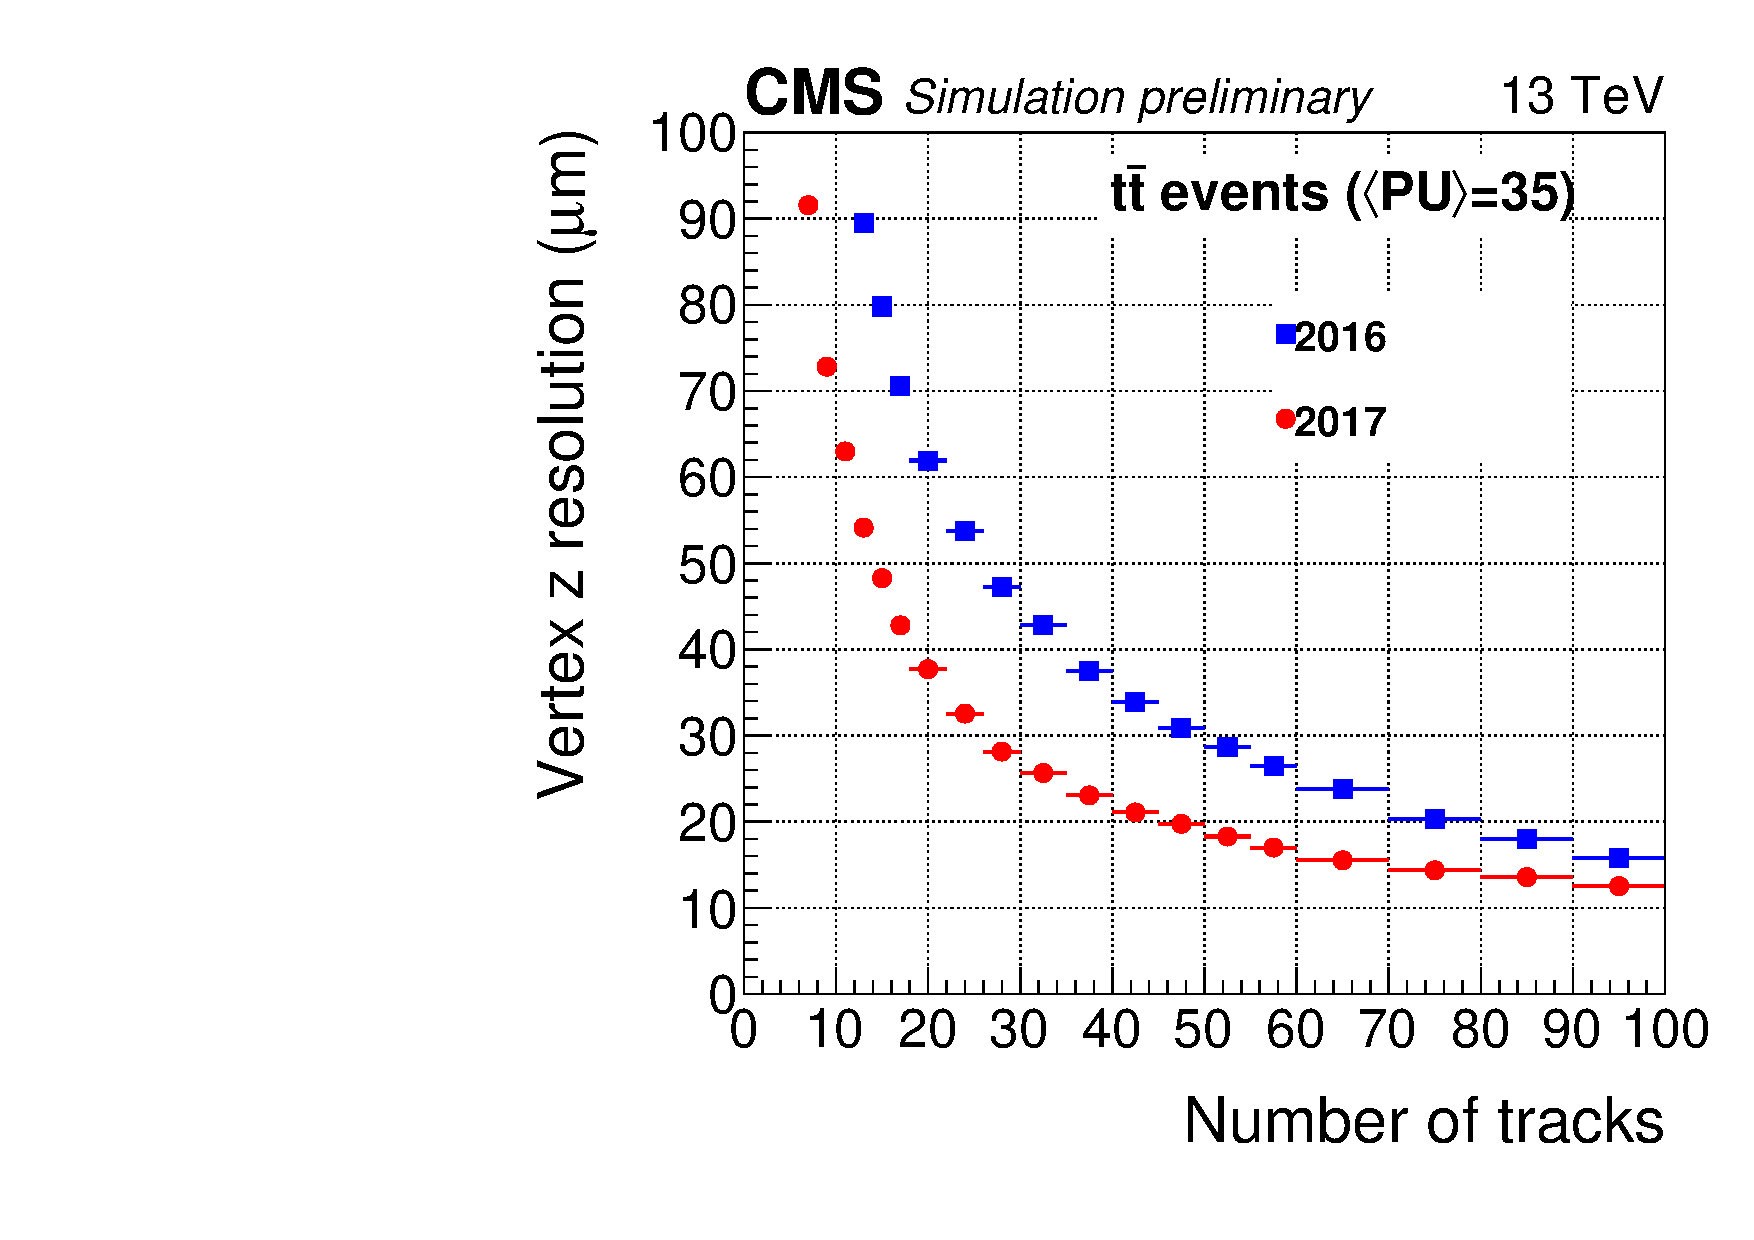
\includegraphics[width=\textwidth]{Figures/Chapter3/Pixel_Vertex_Z_Resolution.pdf}
        \caption{}
    \end{subfigure}
\caption[Vertex resolution comparison between Phase-0 and Phase-1 pixel detectors]{Comparison of the simulated CMS vertex resolution between the Phase-0 and Phase-1 pixel detectors as a function of the number of tracks used in the vertex fit. \textbf{(a)} Transverse ($x,y$) vertex resolution. \textbf{(b)} Longitudinal ($z$) vertex resolution. Figures taken from Ref.~\cite{Pixel_Vertex_Performance}.}

\label{Figure:Chapter3_Pixel_Vertex_Resolution}
\end{figure}


\subsubsection{Silicon Strip Tracker}
Surrounding the pixel detector is the \textbf{\ac{SST}}, illustrated in Fig.~\ref{Figure:Chapter3_Tracker_Geometry}. In the outer tracking region, lower particle occupancy allows the use of silicon strips instead of pixels, relaxing granularity requirements and enabling larger sensor elements. The SST covers an active area of approximately $198\unit{m}^2$ and contains 9.3 million silicon micro-strips distributed across 15,148 detector modules. It is composed of four main subsystems: the \ac{TIB}, \ac{TID}, \ac{TOB}, and \ac{TEC}.

\begin{figure}[h]
\centering
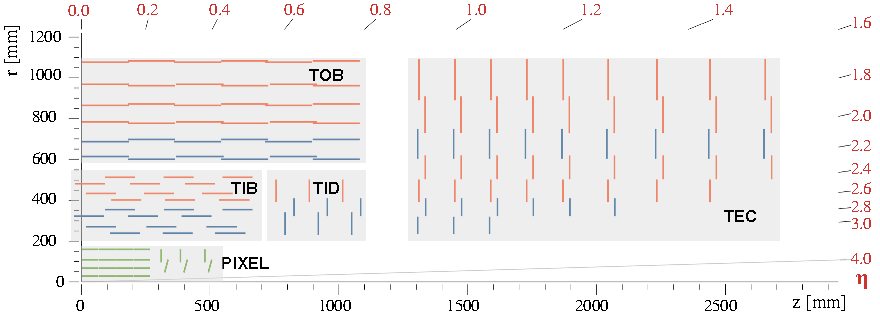
\includegraphics[width=1\textwidth]{Figures/Chapter3/Phase1_Tracker.pdf}
\caption[Schematic of CMS inner tracking system in the $(r-z)$ plane]{Schematic view of one-quarter of the CMS inner tracking system in the $(r-z)$ plane. The pixel detector is depicted in green, located close to the beamline. Single-sided and double-sided strip modules are depicted as red and blue segments, respectively. Figure adjusted from Ref.~\cite{CMS_Detector_Run3}.}
\label{Figure:Chapter3_Tracker_Geometry}
\end{figure}

The \textbf{TIB} is made up of four cylindrical barrel layers located just outside the pixel detector. It provides precise tracking in the central pseudorapidity region and extends out to a radius of $r < 550\unit{mm}$. To ensure complete coverage and continuity in tracking performance, the TIB is complemented by the \textbf{TID}, which consists of three disk-shaped structures at each end of the TIB, extending the longitudinal reach to $|z| < 1180\unit{mm}$. Together, the TIB and TID form the inner part of the strip tracking system, which is crucial for linking tracks from the pixel detector to the outer layers.

The \textbf{TOB} extends the radial coverage beyond the inner systems, occupying the region $r > 550\unit{mm}$. It consists of six cylindrical barrel layers, providing high-precision measurements over a larger area with longer strip modules. The TOB ensures efficient momentum resolution and track reconstruction for particles passing through the outer barrel region, especially those with lower transverse momentum.

The \textbf{TEC} completes the strip tracker by covering the forward pseudorapidity regions. Each TEC consists of nine disks positioned between $1240 < |z| < 2820\unit{mm}$ on either side of the detector. These disks contain up to seven concentric rings of silicon strip modules, which are carefully arranged to maintain uniform tracking performance and coverage up to $|\eta| \simeq 2.5$.

In the barrel sections, the modules are oriented to measure the radial $r\text{-}\phi$ coordinates. Conversely, in the TID and TEC sections, they are primarily aligned to measure $\phi\text{-}z$ coordinates.

In the innermost two layers of the TIB and TOB, the first two rings of the TID, and rings 1, 2, and 5 of the TEC, double-sided modules are deployed. These consist of two single-sided sensors mounted back-to-back with a stereo angle of $100\unit{mrad}$. The combination of their signals enables three-dimensional hit reconstruction, providing an additional measurement of the $z$ coordinate in the barrel and the $r$ coordinate in the disk regions.

\subsection{Electromagnetic calorimeter}

As outlined by the LHC physics requirements in Section~\ref{Section:Chapter3_CMS_Detector_Introduction}, precise reconstruction of electromagnetic particles and robust suppression of background processes ($\pi^0 \to \gamma \gamma$) are essential for CMS. The CMS \textbf{ECAL}~\cite{LHC_CMS,CMS_Detector_Run3,CMS_ECAL_Performance_Run2} is designed to meet these demands, providing high-resolution energy measurements for electrons and photons. It is composed of three main subsystems: a central barrel calorimeter, two endcap calorimeters, and a preshower detector situated in front of the endcaps.

The ECAL is a hermetic homogeneous calorimeter consisting of 61,200 lead tungstate (PbWO$_4$) crystals mounted in the central \textbf{barrel} part. These crystals are arranged in a quasi-projective geometry, with their axes slightly tilted ($3^\circ$) relative to the line from the nominal interaction point. This geometry minimises gaps in the detector and reduces the probability of particles passing through the cracks between crystals. The barrel region covers the pseudorapidity range $|\eta| < 1.479$ and features a 360-fold segmentation in $\phi$ and a ($2 \times 85$)-fold segmentation in $\eta$. Each barrel crystal has a front face cross-section of $22 \times 22\unit{mm}^2$ and a length corresponding to $25.8~X_0$, ensuring that most electromagnetic showers are well-contained within a few crystals.

The \textbf{endcap} region complements the barrel coverage, extending the ECAL acceptance to $1.479 < |\eta| < 3.0$ with 7,324 crystals in each of the two endcaps. These crystals are larger in cross-section ($28.62 \times 28.62\unit{mm}^2$) and slightly shorter in length ($24.7 X_0$) compared to those in the barrel. As in the barrel, the PbWO$_4$ crystals are precisely arranged to maintain fine granularity.

The \textbf{Preshower} system is installed in front of the endcaps, covering a fiducial region of $1.653 < |\eta| < 2.6$. It is designed explicitly for $\pi^0$ rejection by distinguishing between closely spaced photon pairs from $\pi^0 \to \gamma \gamma$ decays. The PS is a $20\unit{cm}$ ($3X_0$) thick sampling calorimeter composed of two alternating layers of lead to initiate electromagnetic showers and silicon strip sensors to measure the deposited energy and transverse shower profiles.

The selection of PbWO$_4$ crystals for all ECAL regions is motivated by their desirable properties: high density ($8.28\unit{gcm}^{-3}$), short radiation length ($0.89\unit{cm}$), and small Moli\`ere radius ($2.2\unit{cm}$). This allows for a compact and granular calorimeter design. Additionally, these crystals emit about 80\% of their scintillation light within $25\unit{ns}$, matching the LHC bunch crossing time and enabling efficient energy collection within a single event window.

A crucial component of the CMS ECAL is the photodetectors, which convert the scintillation light produced in the PbWO$_4$ crystals into electrical signals. Due to the relatively low light yield of these crystals, the photodetectors must provide internal amplification. They must also exhibit a fast response, high radiation tolerance, and compatibility with the strong longitudinal magnetic field of the CMS solenoid ($3.8-4\unit{T}$). \textit{\ac{APDs})} and \textit{\ac{VPTs}} are employed in the barrel and endcap regions, respectively. Although VPTs offer lower quantum efficiency and gain compared to APDs, their exceptional radiation hardness and ability to operate in high-field environments make them well-suited for the endcap configuration.

As shown in Figures~\ref{Figure:Chapter3_CMS_schematic}-\ref{Figure:Chapter3_CMS_slice}, the ECAL is positioned outside the inner tracking system and in front of the hadronic calorimeter. A schematic of the CMS ECAL is shown in Fig.~\ref{Figure:Chapter3_CMS_ECAL}.

\begin{figure}[h]
\centering
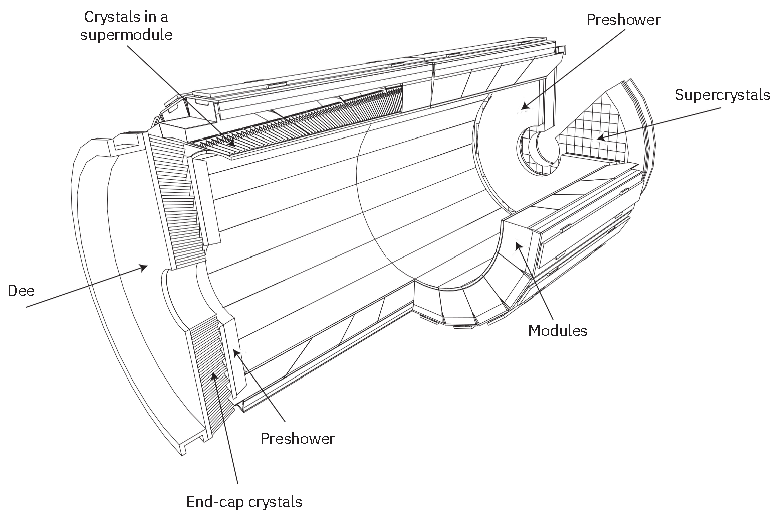
\includegraphics[width= .85\textwidth]{Figures/Chapter3/CMS_ECAL.pdf}
\caption[Schematic view of the CMS ECAL subdetector]{Schematic view of the CMS ECAL subdetector. Figure taken from Ref.~\cite{LHC_CMS}.}
\label{Figure:Chapter3_CMS_ECAL}
\end{figure}
\newpage
The energy resolution of the ECAL is parametrised as a function of the incident particle energy $E$ as:

\begin{equation_pad}
    \left(\frac{\sigma}{E}\right)^2 =  \underbrace{\left(\frac{S}{\sqrt{E}}\right)^2}_{\text{Stochastic}} +  \underbrace{\left(\frac{N}{E}\right)^2}_{\text{Noise}} +  \underbrace{C^2}_{\text{Constant}}
\end{equation_pad}

Each term reflects a different contribution to the resolution: the stochastic term accounts for statistical fluctuations in lateral shower containment and photon yield; the noise term reflects electronic noise and PU; and the constant term arises from detector non-uniformities ($\eg$ longitudinal response) and calibration uncertainties. During an electron test beam in 2014~\cite{ECAL_TestBeam}, the ECAL demonstrated excellent energy resolution, consistent with the design specifications:

\begin{equation_pad}
    \left(\frac{\sigma}{E}\right)^2 =  \underbrace{\left(\frac{2.8\%}{\sqrt{E}}\right)^2}_{\text{Stochastic}} +  \underbrace{\left(\frac{0.12}{E}\right)^2}_{\text{Noise}} +  \underbrace{(0.30\%)^2}_{\text{Constant}}
\end{equation_pad}

\subsection{Hadronic calorimeter}
To complete the calorimetric measurement and ensure accurate reconstruction of hadronic jets and \ac{MET}, the CMS detector employs a dedicated HCAL system. Positioned outside the ECAL, the HCAL is a sampling calorimeter designed to detect strongly interacting particles and spans the pseudorapidity range $|\eta| < 5.2$~\cite{LHC_CMS,CMS_Detector_Run3}. The HCAL comprises four distinct components: the \ac{HB}, \ac{HE}, \ac{HO}, and \ac{HF} calorimeters, as shown in Fig.~\ref{Figure:Chapter3_CMS_HCAL}.

\begin{figure}[h]
\centering
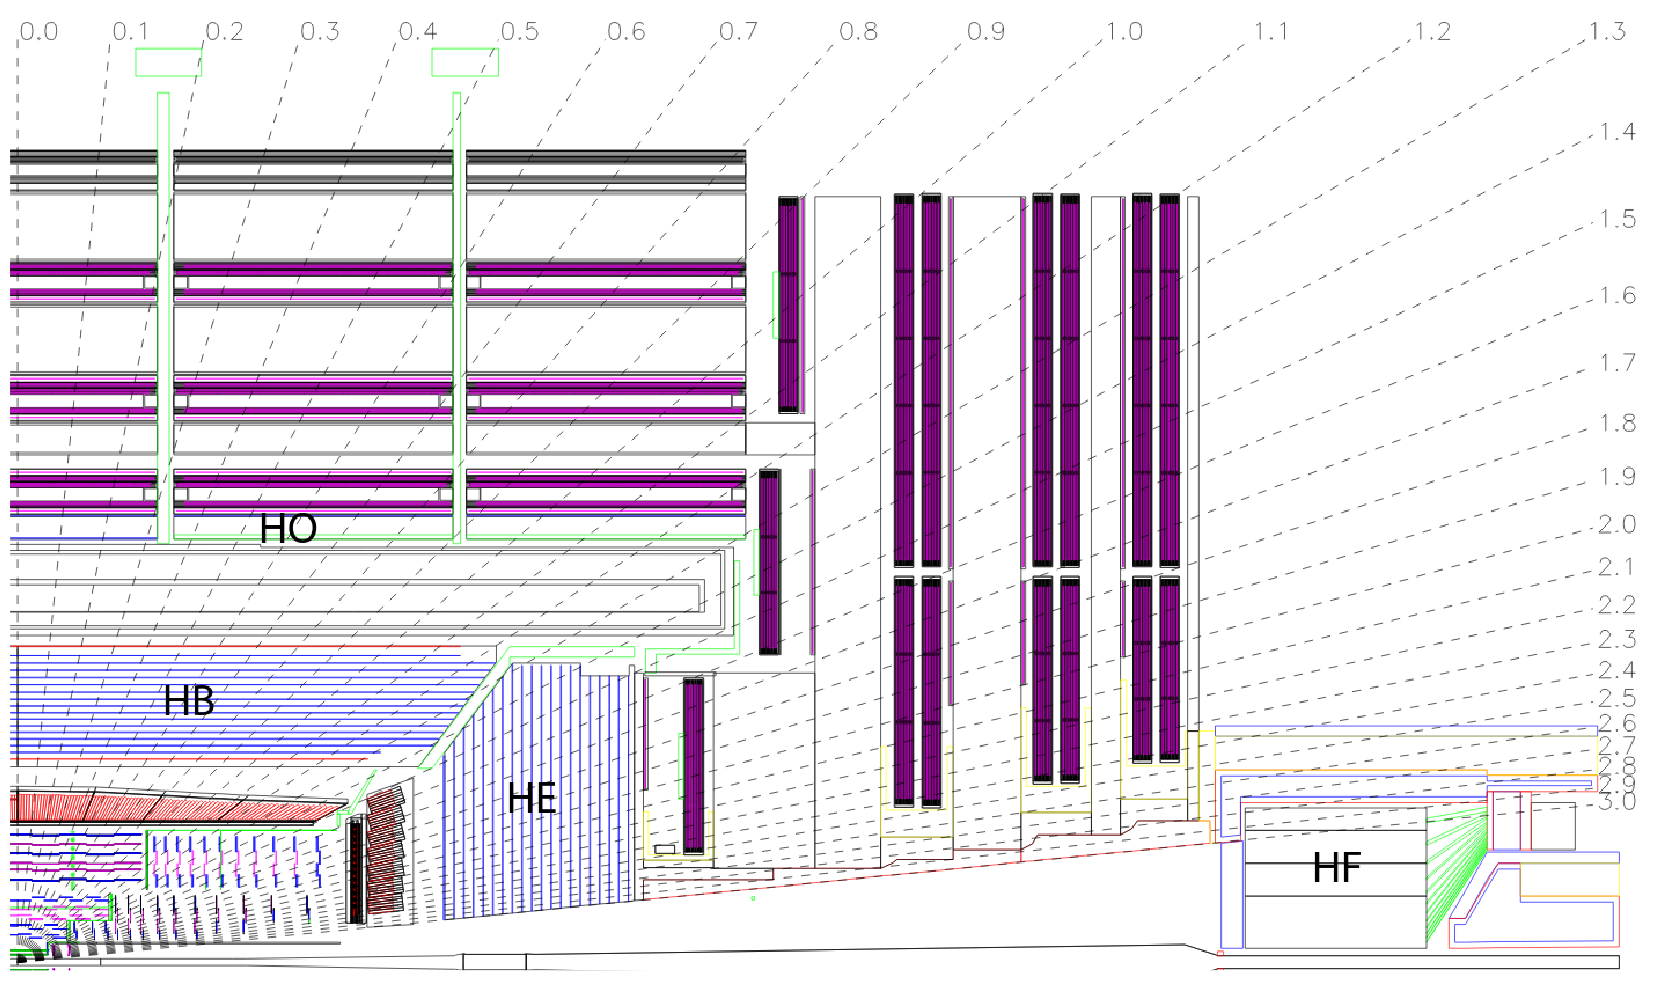
\includegraphics[width= 1.0\textwidth]{Figures/Chapter3/CMS_HCAL.pdf}
\caption[Schematic of CMS detector highlighting HCAL sub-detectors]{A schematic view of one-quarter of the CMS detector with the locations of the HB, HO, HE and HF sub-detectors of the HCAL being shown. Figure adjusted from Ref.~\cite{LHC_CMS}.}
\label{Figure:Chapter3_CMS_HCAL}
\end{figure}

The \textbf{HB} and \textbf{HE} subdetectors are located within the bore of the magnet, covering the pseudorapidity regions $|\eta| < 1.3$ and $1.3 < |\eta| < 3.0$, respectively. They are constructed using alternating layers of brass absorber plates and plastic scintillators. Brass is used due to its short nuclear interaction length and non-magnetic nature, the latter being essential for operation within the CMS solenoid. The HB has a minimum absorber thickness of 5.82 interaction lengths ($\lambda_0$), which increases with polar angle as ($1/\sin\theta$) to approximately 10.6~$\lambda_0$ at $|\eta| = 1.3$. In the \textbf{HE}, 79$\unit{mm}$ thick brass plates interleaved with 9$\unit{mm}$ scintillator gaps provide a total depth of around 10$\lambda_0$, including the contribution from the electromagnetic crystals in front. The calorimeter segmentation is $\Delta\eta \times \Delta\phi = 0.087 \times 0.087$ for $|\eta| < 1.6$, and approximately $0.17 \times 0.17$ for $|\eta| \geq 1.6$. Charged particles from hadronic showers deposit energy in the scintillator tiles, producing scintillation light that is collected by wavelength-shifting fibres and read out using hybrid photodiodes.

Due to the solenoid magnet, the HB is radially restricted, constraining the total amount of material which can be inserted to absorb hadronic showers. As a result, the combined stopping power of the EB and HB does not provide sufficient containment of the hadronic showers. The \textbf{HO} subdetector is used as a tail catcher outside of the solenoid, aiming to ensure adequate sampling depth for $|\eta| < 1.3$. The HO employs the same active scintillator as the HB, while also utilising the solenoid as an additional absorber, extending the minimum depth to 11.8$\lambda_0$. This extended sampling is crucial for identifying and measuring the energy of late-starting or highly penetrating showers.

Beyond $|\eta| < 3.0$, the \textbf{HF} sub-detector extends the pseudorapidity coverage of the CMS HCAL to $|\eta| < 5.2$, and is located at $\pm 11.2\unit{m}$ from the interaction point. Its design posed significant challenges due to the extremely harsh radiation environment in the forward region, where particle fluxes reach unprecedented levels. To ensure long-term durability, the HF was constructed using highly radiation-resistant materials. Quartz fibres were chosen as the active medium, embedded within a steel absorber composed of 5$\unit{mm}$ thick grooved plates into which the fibres are inserted. The HF subdetector is segmented longitudinally into two readout depths: one set of fibres spans the entire 165$\unit{cm}$ depth of the absorber (approximately 10~$\lambda_0$), while the other begins at a depth of 22$\unit{cm}$. By reading out these fibre sets independently, the HF can discriminate between electromagnetic showers, which deposit a large fraction of their energy in the first $22\unit{cm}$ and hadronic showers, which deposit their energy more uniformly across the full depth. When charged particles pass through the quartz fibres, they produce Cherenkov light, which is then collected and transmitted to photomultiplier tubes. The use of Cherenkov light makes the HF relatively insensitive to low-energy particles and neutral backgrounds, such as neutrons or secondary products from activated radionuclides, helping to reduce noise in this high-radiation environment.

When combining information from the inner tracking system with measurements from the calorimeters, the jet energy resolution typically reaches 15\% at $10\unit{GeV}$, 8\% at $100\unit{GeV}$, and 4\% at $1\unit{TeV}$. In comparison, using only the ECAL and HCAL calorimeters yields resolutions of approximately 40\%, 12\%, and 5\% at the same energies, respectively~\cite{CMS_HCAL_EnergyResolution}.

\subsection{Muon system}
To satisfy the LHC’s stringent performance goals for muon reconstruction, CMS employs a dedicated muon tracking system~\cite{LHC_CMS,CMS_Muon_System_Performance} positioned furthest from the interaction point. The system serves three primary functions: muon identification, momentum measurement, and triggering. These are made possible by the strong solenoidal magnetic field and the iron return yoke, which acts as a hadron absorber.  CMS employs three complementary gaseous particle detector technologies for detecting muons.  

In the barrel region, where muon rates and neutron-induced backgrounds are relatively low, the $3.8–4\unit{T}$ magnetic field is uniform and largely confined within the iron yoke. \textbf{\ac{DTs}} are used here, providing coverage in the pseudorapidity region $|\eta| < 1.2$. These are organised into four stations interspersed among the layers of the flux return plates. The first three stations are further subdivided into eight chambers, four measuring the muon coordinate in the $r-–\phi$ bending plane and four providing a measurement in the $z$ direction. Conversely, the capabilities of the fourth muon station are restricted to $r–-\phi$ measurements. Each DT chamber consists of rectangular drift cells containing a central anode wire. The cells are filled with a gas mixture of argon and carbon dioxide, which enables efficient ionisation and drift of electrons toward the wire for signal detection. 

In contrast to the barrel region, the endcaps are subjected to higher muon rates and background levels. The magnetic field in this region is both strong and non-uniform, necessitating a finely segmented detector system that is radiation-resistant and capable of fast response times. To meet these demands, CMS employs \textbf{\ac{CSCs}} in the region $0.9 < |\eta|<2.4$. Each CSC is a multi-layered gaseous detector consisting of six planes of anode wires interleaved with seven cathode layers. In both endcaps, the chambers are arranged into four stations placed perpendicular to the beam line and embedded between the layers of the iron yoke. The cathode strips extend radially outward from the beam axis, providing precise position measurements in the $r-\phi$ plane. The anode wires, oriented roughly perpendicular to the strips, deliver additional spatial information in $\eta$ and enable timing measurements relative to the beam crossing. This six-layer configuration enhances pattern recognition, improving the rejection of spurious hits from background sources and allowing for efficient correlation with hits from other stations and with tracks reconstructed in the inner tracker.

The DT and CSC systems are complemented by the \textbf{\ac{RPC}} system in the pseudorapidity region $|\eta| < 1.6$. RPCs are double-gap chambers featuring anode and cathode plates separated by gas. Compared to DTs and CSCs, RPCs exhibit lower granularity; however, they offer a faster response and good time resolution. These characteristics make them particularly well-suited for use as trigger detectors. As such, they are especially valuable in scenarios where the DT and CSC systems may struggle to cope with PU-induced background. Additionally, RPCs contribute to resolving ambiguities when reconstructing tracks from multiple hits within a chamber, further enhancing the overall performance of the muon detection system.

A schematic illustration of the CMS muon detection system is shown in Fig.~\ref{Figure:Chapter3_CMS_Muon_System}, highlighting the arrangement of the DT, CSC, and RPC subdetectors within the return yoke. Owing to its design, the CMS muon system achieves a reconstruction and identification efficiency exceeding 95\% for muons with energies above a few $\unit{GeV}$. The momentum resolution varies between 1\% and 6\% for transverse momenta below $100\unit{GeV}$, and remains better than 10\% up to $1\unit{TeV}$~\cite{CMS_Muon_System_Performance_2}. Furthermore, the system reliably determines the muon charge sign for transverse momenta up to $1\unit{TeV}$.


\begin{figure}[h]
\centering
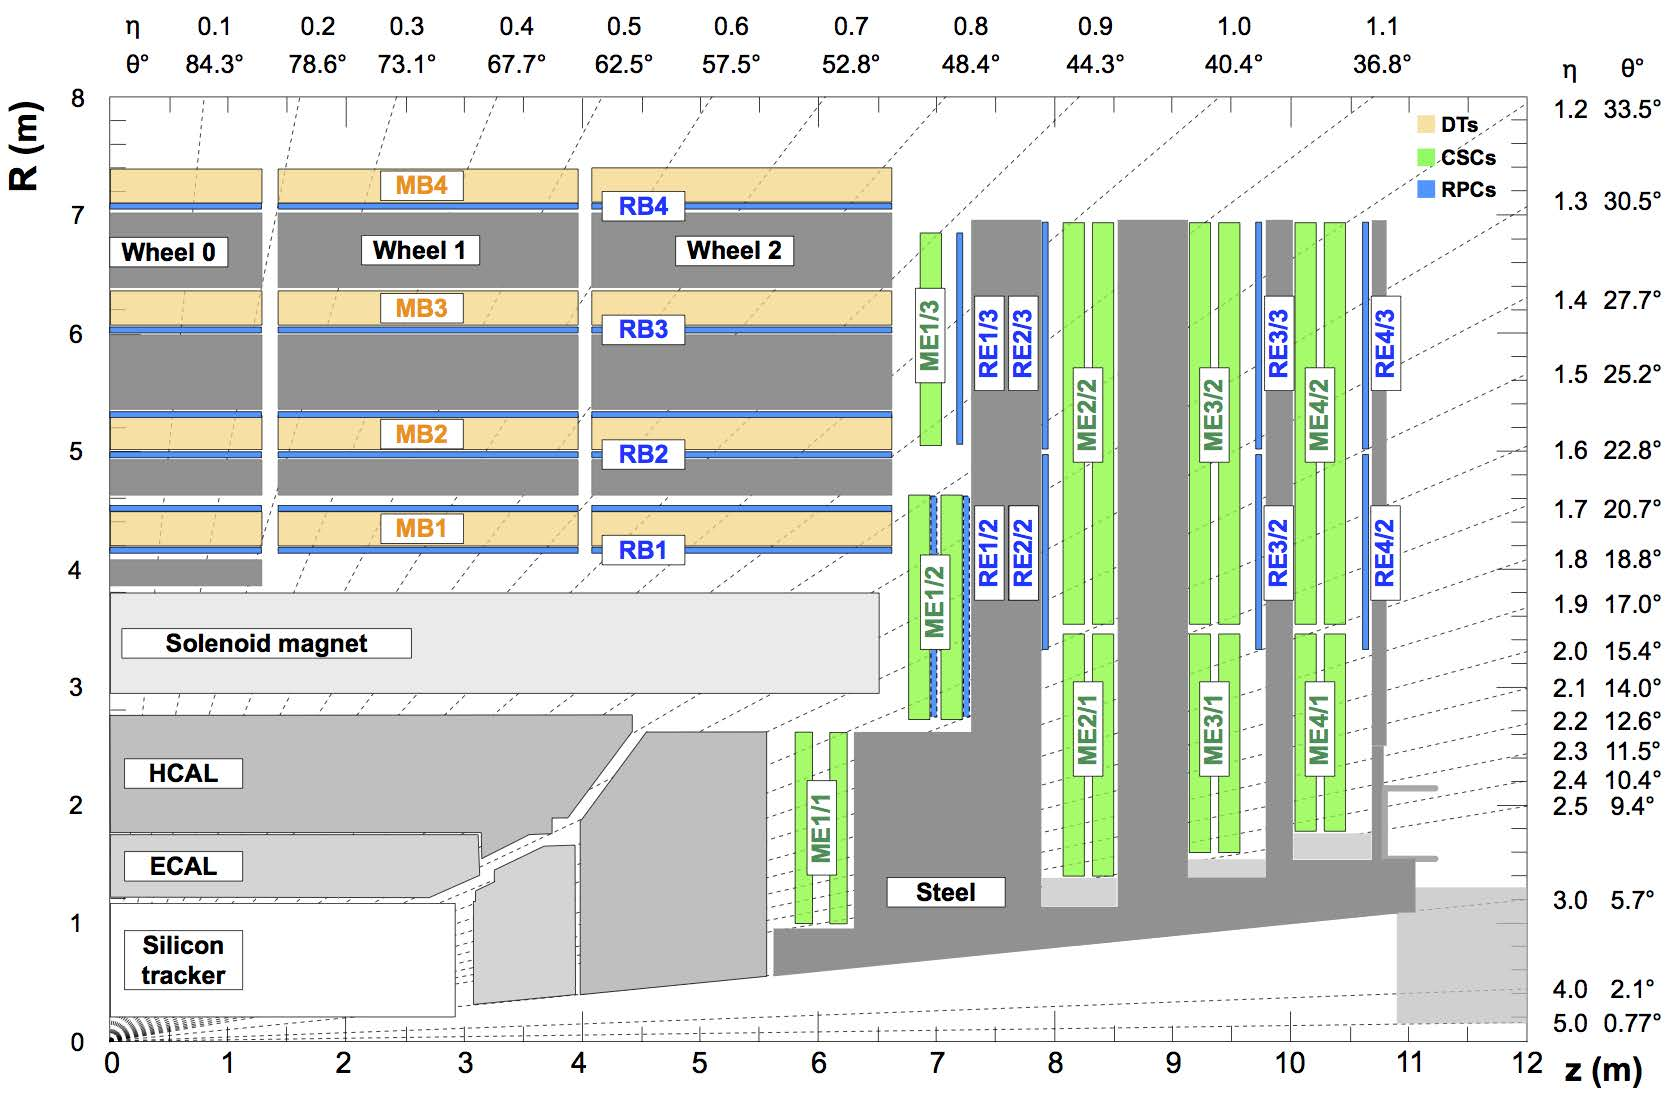
\includegraphics[width= 1.0\textwidth]{Figures/Chapter3/CMS_Muon_System.pdf}
\caption[Schematic of CMS muon detection system]{Schematic illustration of one quarter of the CMS detector, highlighting the muon detection system. The DT stations are labelled as MB (Muon Barrel), while the CSCs are labelled as ME (Muon Endcap). The RPCs are denoted as RB in the barrel region and RE in the endcap region. Figure taken from Ref.~\cite{CMS_Muon_System_Performance}.}
\label{Figure:Chapter3_CMS_Muon_System}
\end{figure}

\subsection{Trigger system}

At the LHC interaction points, proton bunches cross every $25\unit{ns}$, resulting in a nominal bunch crossing frequency of $40\unit{MHz}$. Additionally, each bunch crossing can yield up to more than 50~PU interactions corresponding to an aggregate rate of individual proton-proton interactions surpassing $1\unit{GHz}$. Recording all of these collisions is not feasible nor necessary, as only a small fraction contains events of interest to the CMS physics programme. To select the most interesting events, CMS employs a dedicated two-level trigger system~\cite{CMS_Trigger} consisting of the \textbf{\ac{L1} trigger} and the \textbf{\ac{HLT}}.

As the name suggests, the \textbf{L1 trigger} is the first level of the CMS trigger system, implemented as a hardware-based trigger on custom-built Field Programmable Gate Arrays with a fixed latency of $4\unit{\mu s}$. CMS relies on this system to rapidly determine whether an event should be tentatively accepted or rejected based on calorimeter energy deposits and muon detector hits. The L1 decision chain comprises three primary subsystems: the L1 calorimeter system, the L1 muon trigger system and the global trigger (GT), as shown in Fig.~\ref{Figure:Chapter3_CMS_L1_Trigger}.

\begin{figure}[h]
\centering
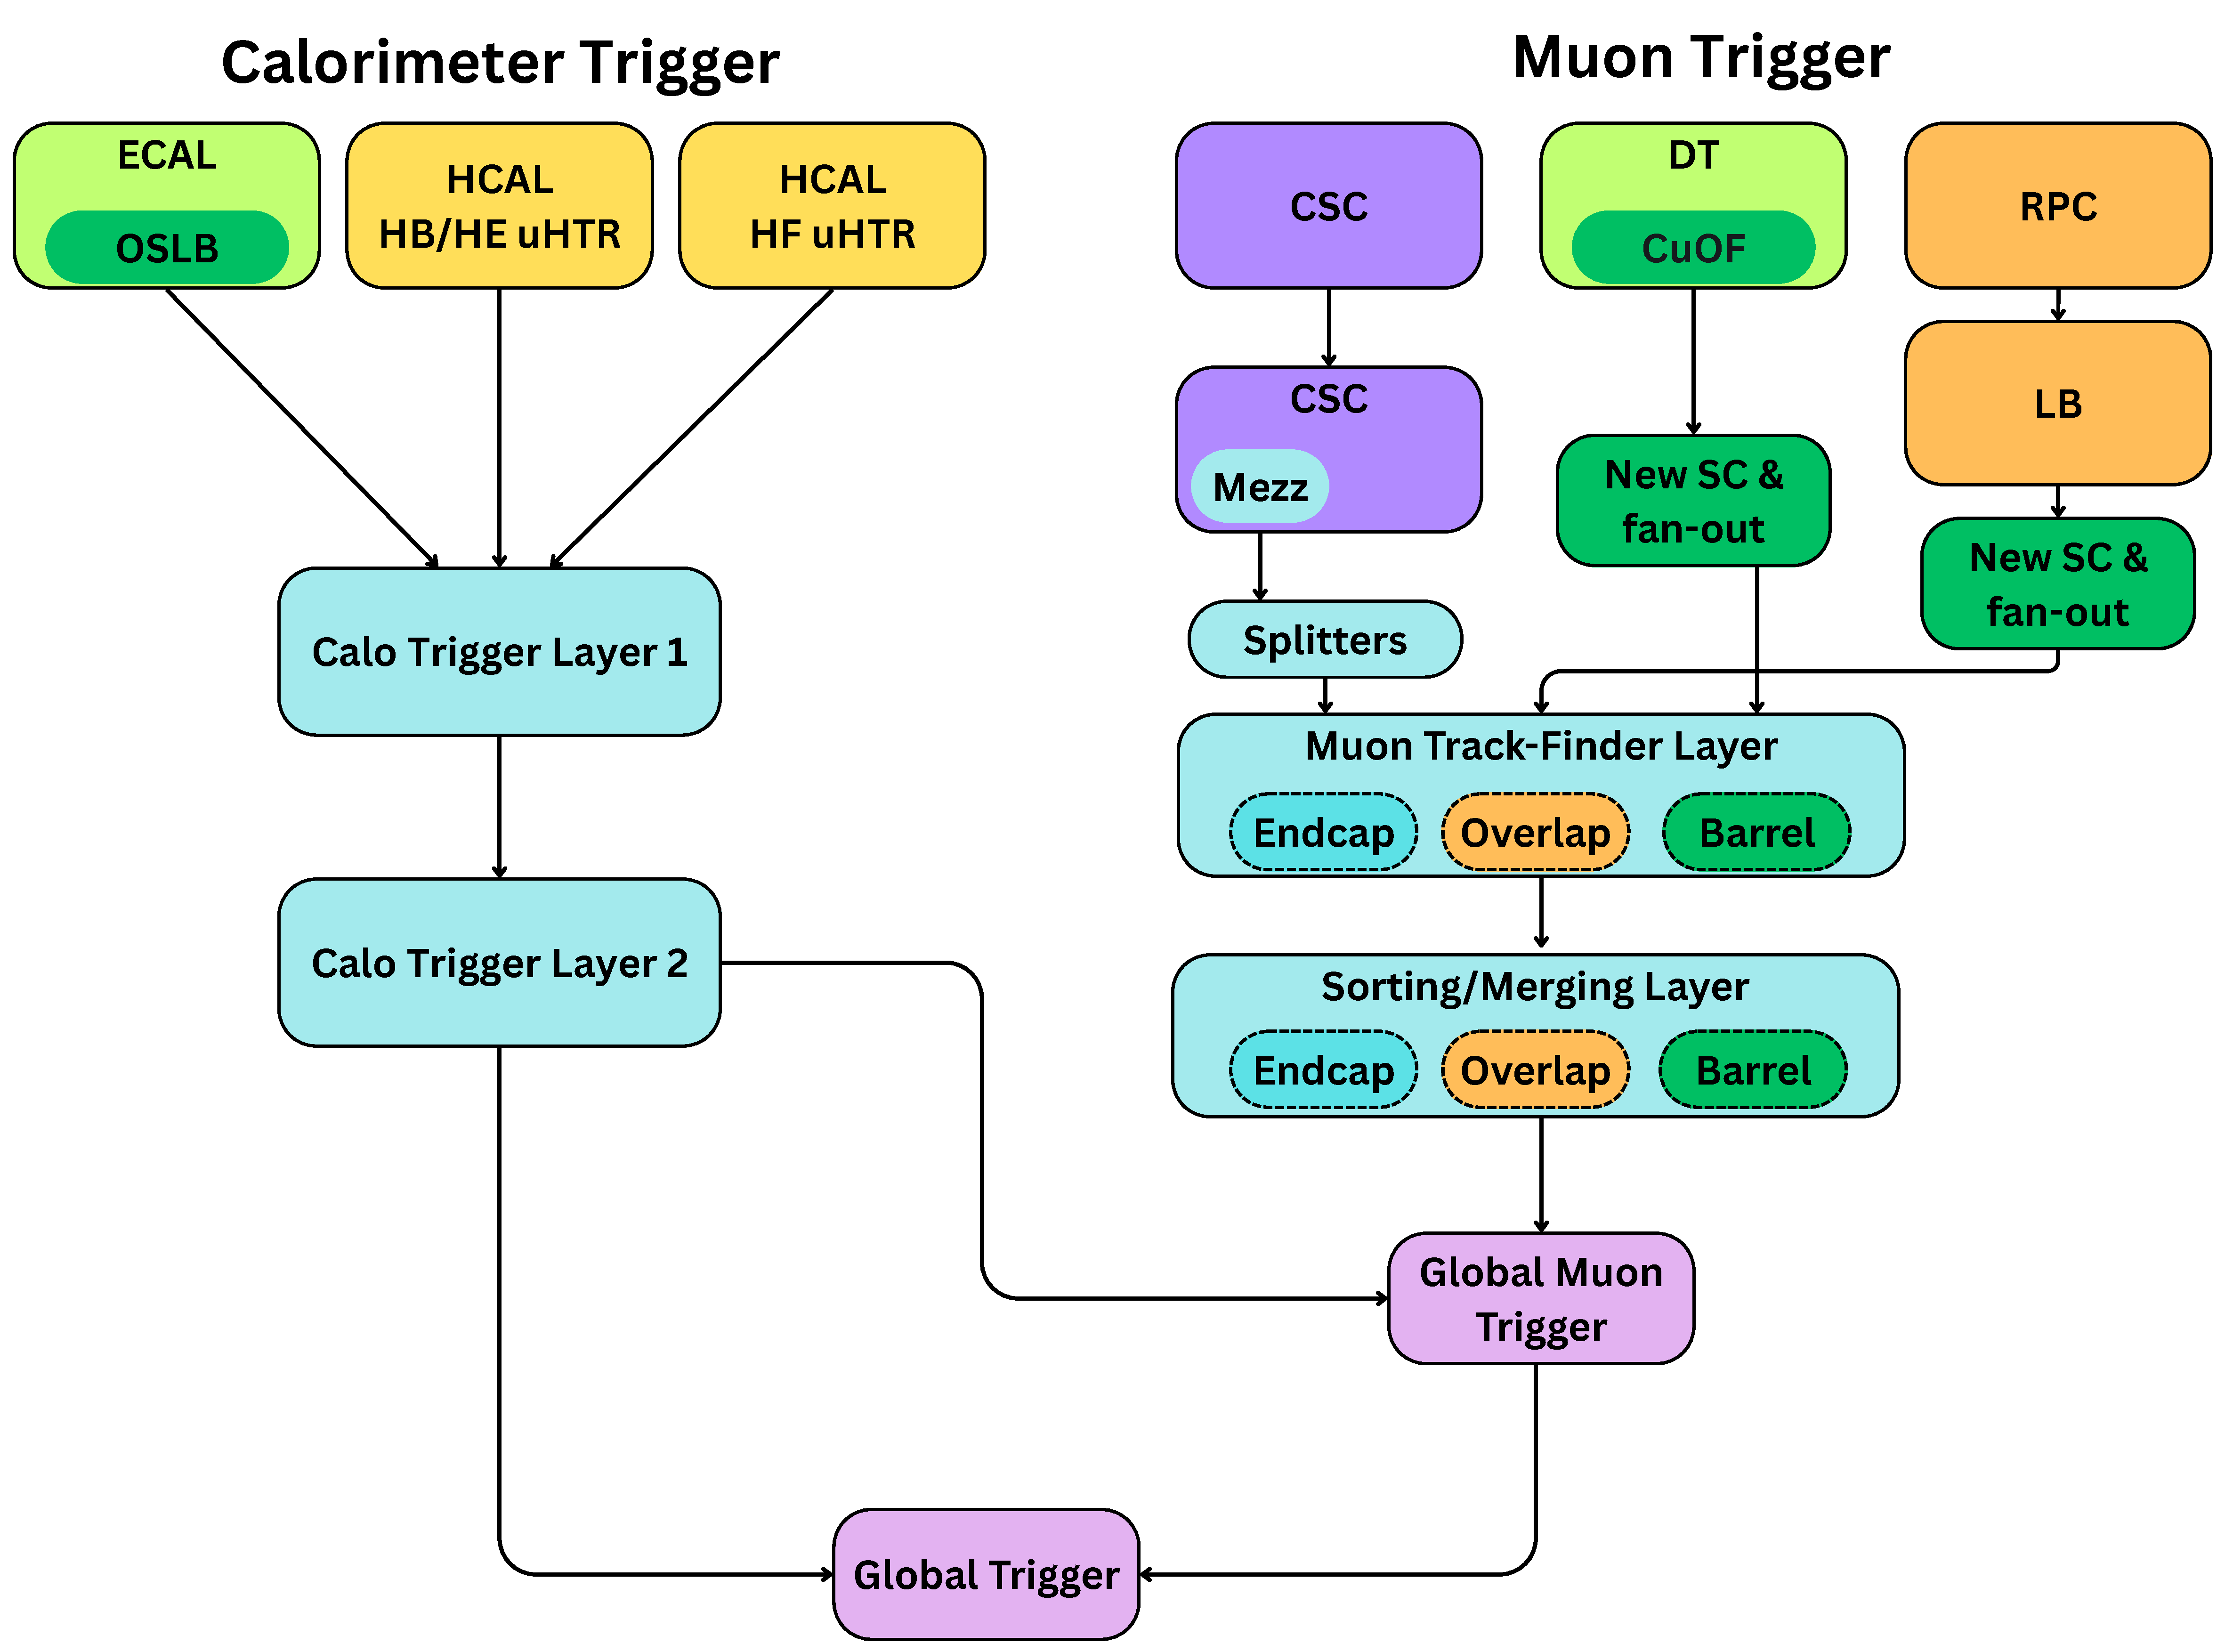
\includegraphics[width= 1.0\textwidth]{Figures/Chapter3/CMS_L1_Trigger.pdf}
\caption[Schematic of the CMS L1 trigger workflow]{Schematic of the CMS L1 trigger workflow. Figure reproduced from Ref.~\cite{CMS_L1_Trigger}.}
\label{Figure:Chapter3_CMS_L1_Trigger}
\end{figure}

The \textbf{L1 calorimeter trigger system} is organised into two processing layers. Layer-1 (\textit{Calo Trigger Layer 1}) receives trigger primitives (energy deposits) from the ECAL and the HCAL, performs initial calibrations, and sorts local energy deposits. Layer-2 (\textit{Calo Trigger Layer 2}) processes the calibrated information to reconstruct and further calibrate high-level physics objects such as electrons, photons, jets, taus, and MET. Simultaneously, hits from the three muon subsystems are processed by the first stage of the \textbf{L1 muon trigger system} (\textit{Muon Tracking-Finder Layer}). At this stage, track finding is performed by combining hits within sectors in $\phi$ and $\eta$. The reconstructed track candidates are then forwarded to the \textit{Sorting and Merging Layer}, where information from the $\phi$ sectors is consolidated. The output, along with the calorimeter information required to compute isolation, is passed to the global muon trigger, where a sorted list of muon candidates for the entire detector is produced. Finally, the \textbf{global trigger} integrates the information from both the L1 calorimeter and muon trigger systems, enabling it to make a decision on the fate of the event. This allows for the event rate to be reduced from $40\unit{MHz}$ to $100\unit{kHz}$.

The \textbf{HLT} system is the second stage of the CMS trigger architecture. It is a software-based trigger that runs on a processor farm composed of commercial CPUs. In contrast to the hardware-based L1 trigger, the HLT utilises full-resolution data from the CMS detector and applies offline-quality reconstruction algorithms for more refined event selection. The primary objective of the HLT is to further reduce the event rate to about $1\unit{kHz}$ for permanent storage and offline analysis. 

Rather than operating with fixed latency, the HLT processes events asynchronously, scaling with available CPU resources. Its workflow is organised into HLT paths, each consisting of a predefined sequence of algorithmic steps that reconstruct and select physics objects. These paths are structured to increase in complexity, precision, and physics sophistication. To optimise computational efficiency, initial selections use fast information from the calorimeters and muon detectors, while CPU-intensive tracking is applied only to events that pass these preliminary filters. 

Events accepted by the HLT are handed off to the storage manager, which writes them temporarily to local disk. They are then transferred to the CMS Tier‑0 computing centre for offline reconstruction and long‑term archival.



\setcounter{mtc}{4}
\chapter{XXXXXX}
\chaptermark{XXXXX}  
\thispagestyle{plain}  % First page has default style
\pagestyle{chapterpages}
\label{Section:Chapter4}

\minitoc

hey hey
% \chapter{The Compact Muon Solenoid experiment}
% \section{Introduction}
% \section{The Large Hadron Collider}
% \section{The CMS detector}
% \subsection{Coordinate system}
% \subsection{Tracker}
% \subsection{Electromagnetic calorimeter}
% \subsection{Hadronic calorimeter}
% \subsection{Superconducting solenoid}
% \subsection{Muon system}
% \subsection{Trigger system and computing}
% \subsubsection{RAW and RAW' Data Format}

% \chapter{Object reconstruction}
% \section{Tracks and vertices}
% \section{Particle flow}
% \section{Muons}
% \section{Electrons}
% \section{Jets}
% \section{b-jets}
% \section{Missing transverse energy}
% \section{Hadronic Tau identification}
% \subsection{Hadron-plus-strip algorithm}
% \subsection{Misidentification of hadronic taus}
% \subsection{DeepTau}

% \chapter{Search for new physics in aa final states}
% \section{Signal modelling}
% \section{Event selection}
% \subsection{Trigger requirements}
% \subsection{Offline requirements}
% \section{Background modelling}
% \subsection{Genuine Backgrounds}
% \subsubsection{Uncertainty model}
% \subsection{Jets misidentified as hadronic tau candidates}
% \subsubsection{Uncertainty model}
% \section{Systematic uncertainties}
% \subsection{Normalisation uncertainties}
% \subsection{Shape uncertainties}
% \section{Analysis optimisation}
% \section{Signal extraction and statistical interpretation}
% \section{Model independent results}
% \section{Model dependent results}

% \chapter{Measurements of Higgs boson CP properties}
% \section{Acoplanarity angle reconstruction}
% \subsection{Impact Parameter method}
% \subsection{Neutral Pion method}
% \subsection{Polarimetric Vector method}
% \section{Signal modelling}
% \section{Event selection}
% \section{Background modelling}
% \subsection{Genuine backgrounds}
% \subsection{Jets misidentified as hadronic tau candidates}
% \section{Systematic uncertainties}
% \subsection{Normalisation uncertainties}
% \subsection{Shape uncertainties}
% \section{Analysis optimisation}
% \section{Measurement procedure and statistical interpretation}
% \section{Results}

% \chapter{Conclusions}

\addcontentsline{toc}{chapter} {Supplementary Material}

\addcontentsline{lot}{table}{Phantom Table}
\addcontentsline{lof}{figure}{Phantom Figure}

% \begin{figure}
% \centering
% \subfloat[Amazon]{\label{amazon}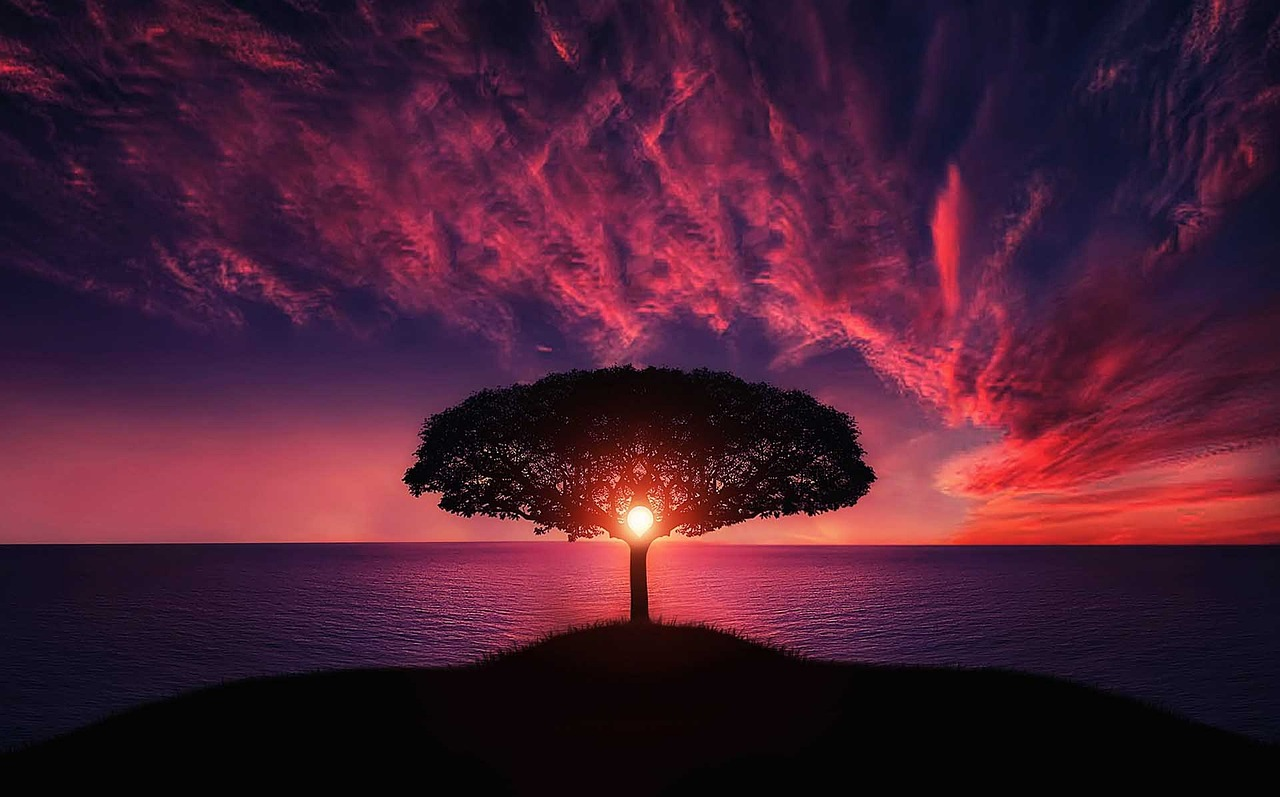
\includegraphics[width= 0.48\textwidth]{Chapter2/1.jpg}} \quad
% \subfloat[Nile]{\label{nile}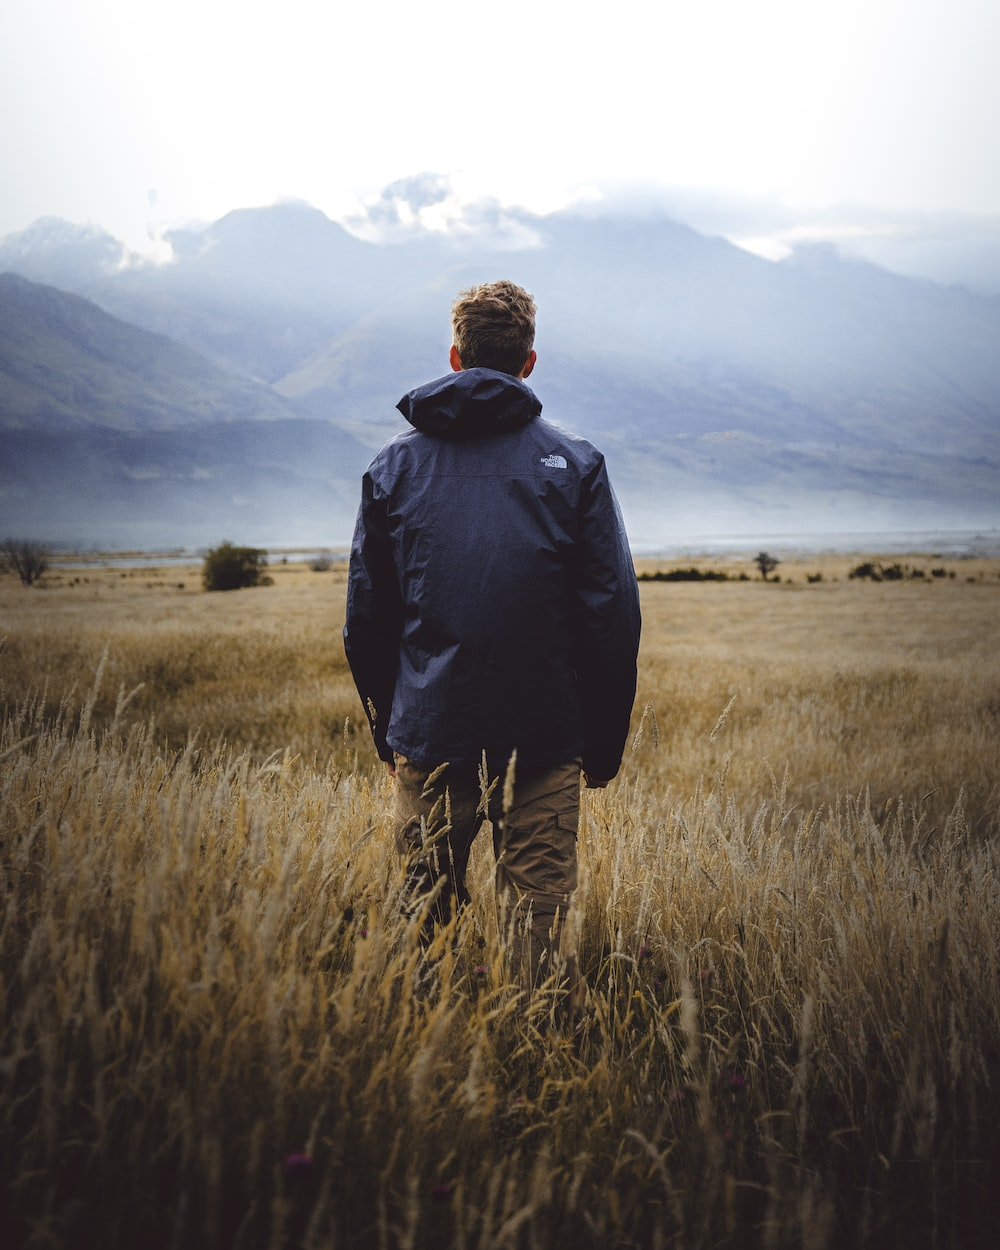
\includegraphics[width= 0.48\textwidth]{Chapter2/2.jpeg}} \\ 
% \subfloat[Yangtze]{\label{yangtze}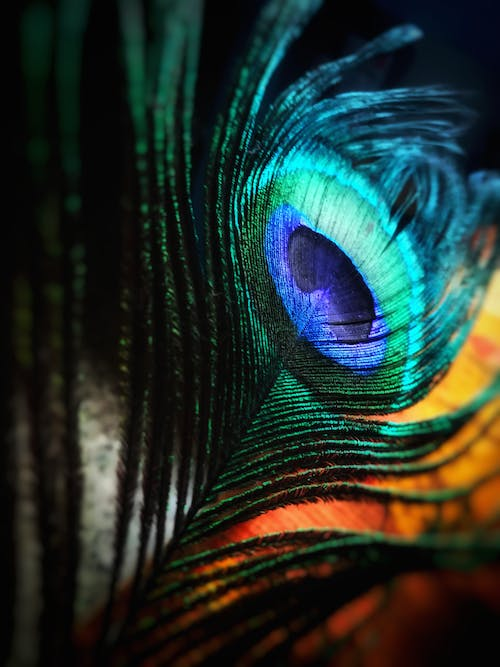
\includegraphics[width= 0.52\textwidth]{Chapter2/3.jpeg}} \quad
% \subfloat[Thames]{\label{thames}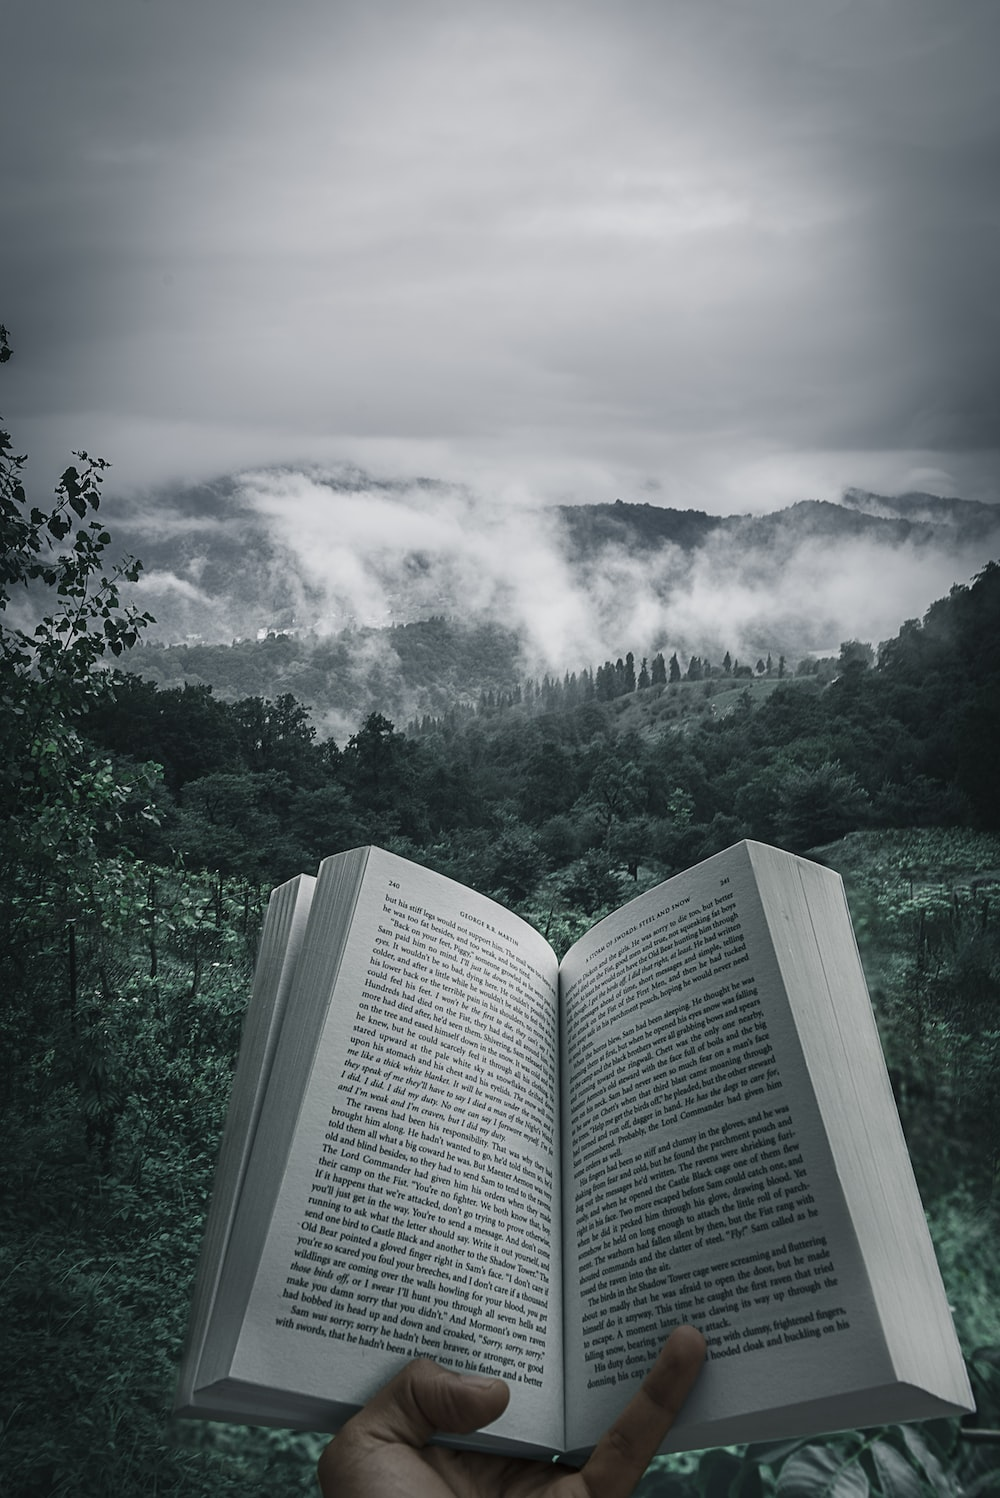
\includegraphics[width= 0.44\textwidth]{Chapter2/4.jpeg}}
% \caption{Rivers}\label{rivers}
% \end{figure}

% \ref{nile} is part of \ref{rivers}.
% \clearpage
% $\diff{y}{x}=\hardmaths$

% \clearpage
% \blindtext
% \begin{singlespace}
% \blindtext
% \end{singlespace}
% \blindtext\footnote{\blindtext}




% \section{Main Section}
% You may often find it useful to use a \ac{TLA}. Nothing is more useful that a \ac{TLA}, except many \acp{TLA}. \ac{ICL} is a good \ac{TLA}.

% \begin{alignat}{2}
% y=&4x \quad & \textrm{for } x < 0\\
% y=&4x+x^{2}-5x^{3} \quad & \textrm{otherwise}\\
% \diff{x}{t}=& 3y\\
% x(t=0)=&-10
% \end{alignat}

% \section{Validation of the acoplanarity angle reconstruction}

\bibliographystyle{unsrtnat}
\bibliography{myrefs}
\end{document}
